\providecommand{\toplevelprefix}{../..}  % necessary for subfile bibliography + figures compilation to work, do not move this after documentclass
\documentclass[../../book-main.tex]{subfiles}
\usepackage[UTF8]{ctex}
\graphicspath{{\subfix{../..}}}

\begin{document}

\chapter{通过有损压缩寻求低维分布}
\label{ch:compression}\label{ch:general-distribution}

\begin{quote}
	\hfill    “{\em 我们为学习而压缩,我们为压缩而学习。}”\\
	$~$ \hfill --- 《高维数据分析》,Wright and Ma, 2022
\end{quote}
\vspace{5mm}

在章节 \ref{ch:linear-independent} 中,我们已经展示了如何学习简单类别的分布,这些分布的支撑集被假设为单个或混合的低维子空间或低秩高斯分布。为了进一步简化,不同的(隐藏)线性或高斯模式被假设为正交或独立的\footnote{或者可以很容易地简化为这种理想情况。},如图 \ref{fig:subspaces} 所示。正如我们所展示的,对于这类特殊分布,可以推导出相当简单有效的学习算法,并带有正确性和效率的保证。相关算法中操作的几何和统计解释也非常清晰。

在实践中,线性和独立性都是相当理想化的假设,现实世界高维数据的分布很少满足这些假设。我们唯一可以假设的是,分布的内在维度远低于数据嵌入的环境空间的维度。因此,在本章中,我们将展示如何学习高维空间中更普遍的一类低维分布,这些分布不一定是(分段)线性的。

现实数据的分布通常包含多个成分或模式,例如在图像中对应不同类别的对象。这些模式在统计上可能不是独立的,它们甚至可能具有不同的内在维度。同样典型的是,我们只能接触到分布的有限数量的样本。因此,总的来说,我们可以假设我们的数据分布在高维空间中的(非线性)低维子流形的混合体上。图 \ref{fig:mixture-manifolds} 展示了这样一个分布的例子。

在这样的条件下学习这样一个分布,我们需要解决几个基本问题:
\begin{itemize}
	\item 学习高维空间中一个普遍的低维分布并表示所学分布的通用方法是什么?
	\item 我们如何衡量所得表示的复杂性,以便我们能有效地利用低维性进行学习?
	\item 我们如何使学习过程在计算上易于处理甚至可扩展,因为环境维度通常很高,样本数量通常很大?
\end{itemize}
正如我们将看到的,{\em 压缩}或{\em 降维}的基本思想,在处理线性和独立情况时已被证明非常有效,它仍然是为学习普遍低维分布开发有效计算模型和方法的通用原则。

由于其理论和实践意义,我们将更深入地研究当感兴趣的分布可以被低维子空间或低秩高斯的混合体很好地建模或近似时,这个通过压缩学习低维分布的通用框架是如何具体化的。
%\yima{I did not touch the above introduction. We can rewrite it when the rest of the chapter is stable. But should state the purpose clearly: a computional framework that strives for achievable and implementable compressive encoding and decoding schemes!}

\begin{figure}
    \centering
    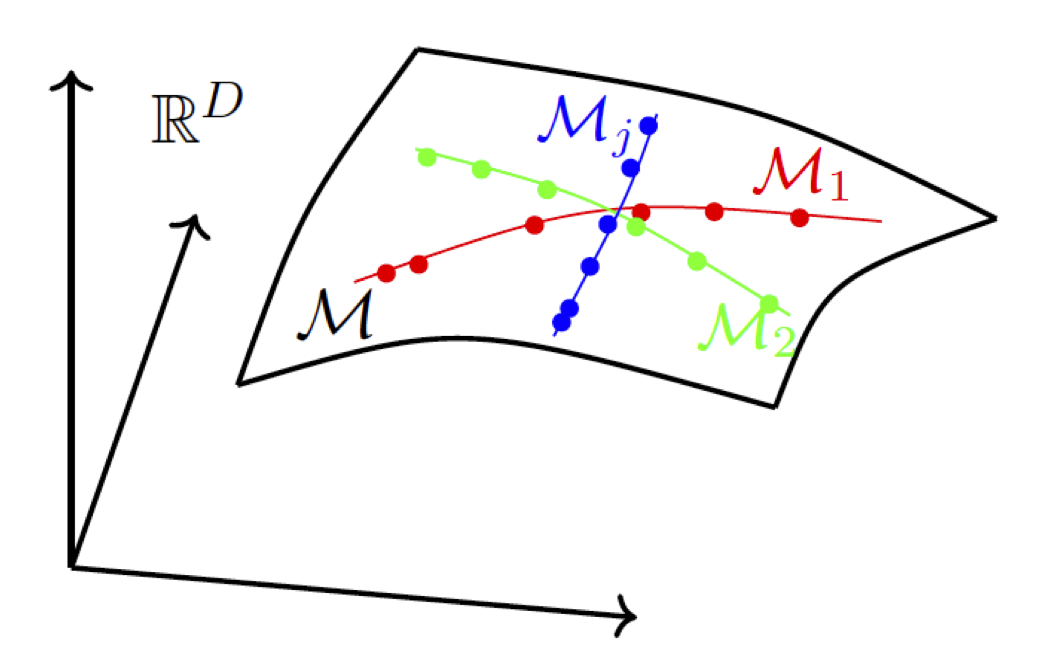
\includegraphics[width=0.5\linewidth]{\toplevelprefix/chapters/chapter3/figs/mixed-manifolds.png}
    \caption{数据分布在一个非常高维的环境空间(比如 $\mathbb{R}^D$)中的低维子流形 $\cup_j \mathcal{M}_j$ 的混合体上。}
    \label{fig:mixture-manifolds}
\end{figure}


\section{熵最小化与压缩}

\subsection{熵与编码率}
在章节 \ref{ch:intro} 中,我们提到学习的目标是找到生成给定数据集的最简单方法。从概念上讲,柯尔莫哥洛夫复杂性旨在提供这样一种复杂性度量,但它是不可计算的,并且与任何可以实际再现数据的可实现方案无关。因此,我们需要一个可替代的、可计算的、可实现的复杂性度量。这就引出了由香农在1948年引入的{\em 熵}的概念 \cite{Shannon-1948}。

为了说明熵的构造性,让我们从最简单的情况开始。假设我们有一个离散随机变量,它以相等的概率 $1/N$ 取 $N$ 个不同的值或\textit{符号},$\{\x_1, \ldots, \x_N\}$。那么我们可以用 \(i\) 的 \(\log_2 N\) 位二进制表示来编码每个符号 \(\vx_{i}\)。这种编码方案可以推广到编码任意离散分布 \cite{Cover-Thomas}:给定一个分布 \(p\) 使得 $\sum_{i=1}^N p(\x_i) = 1$,可以为每个概率为 $p(\x_i)$ 的符号 $\x_i$ 分配一个大小为 $\log_2 [1/p(\x_i)] = - \log_2 p(\x_i)$ 位的二进制码。因此,编码来自该分布 $p(\cdot)$ 的任何样本所需的平均位数,或称{\em 编码率},由以下表达式给出:\footnote{根据信息论的惯例 \cite{Cover-Thomas},这里的 $\log$ 是以2为底的。因此,熵以(二进制)比特为单位。}
\begin{equation}
	H(\x) \doteq \mathbb{E}[\log 1/p(\x)]  = - \sum_{i=1}^N p(\x_i) \log  p(\x_i).
	\label{eqn:entropy-discrete}
\end{equation}
这被称为(离散)分布 $p(\cdot)$ 的{\em 熵}。注意,这个熵总是非负的,并且当且仅当对于某个 $i \in [N]$ 有 $p(\x_i) = 1$ 时,它才为零。\footnote{这里我们利用了事实 $\lim_{p\rightarrow 0} p \log p = 0$。}


\subsection{微分熵}

当随机变量 $\x \in \R^{D}$ 是连续的并且具有概率密度 $p$ 时,可以将上述和 \eqref{eqn:entropy-discrete} 的极限看作与一个积分相关:
\begin{equation}
	h(\vx) \doteq \Ex[\log 1/p(\vx)] = - \int_{\R^{D}} p(\vxi) \log p(\vxi) \odif{\vxi}.
	\label{eqn:entropy-differential}
\end{equation}
{更准确地说,给定一个连续变量 $\x$,我们可以用一个量化大小 $\epsilon > 0$ 对其进行量化。将得到的离散变量表示为 $\x^\epsilon$。那么可以证明 $H(\vx^\epsilon) + \log(\epsilon) \approx h(\vx)$。因此,当 $\epsilon$ 很小时,微分熵 $h(\x)$ 可以是负的。感兴趣的读者可以参考 \cite{Cover-Thomas} 获取更详细的解释。}

\begin{example}[高斯分布的熵]
	通过直接计算,可以证明高斯分布 $x \sim \mathcal{N}(\mu, \sigma^2)$ 的熵由下式给出:
	\begin{equation}
		h(x) = \frac{1}{2}\log (2\pi \sigma^2) + \frac{1}{2}.
		\label{eqn:entropy-Gaussian}
	\end{equation}
	还已知,对于所有具有相同方差 $\sigma^2$ 的分布,高斯分布的熵最大。在 $\mathbb{R}^D$ 中的多元高斯分布 $\x \sim \mathcal{N}(\boldsymbol{\mu}, \boldsymbol{\Sigma})$ 的熵由下式给出:
	\begin{equation}
		h(\x) = \frac{D}{2}(1 + \log(2\pi)) + \frac{1}{2}\log\det(\boldsymbol{\Sigma}).
		\label{eqn:entropy-Gaussian-multi}
	\end{equation}
\end{example}

与离散分布的熵类似,我们希望微分熵与某个可实现的编码方案的编码率相关联。例如,如上所述,我们可以用大小为 $\epsilon >0$ 的网格来离散化分布的域。所得离散分布的编码率可以看作是微分熵的近似 \cite{Cover-Thomas}。


需要注意的是,微分熵的定义存在一些需要注意的地方。对于高维空间中的分布,当其支撑集变得退化(低维)时,其微分熵会发散到 \(-\infty\)。这一事实在 \Cref{thm:max_entropy} 中得到证明(我们也在 \Cref{thm:max_entropy} 中回顾了前面提到的高斯分布的最大熵特性),但即使在简单明确的高斯分布情况 \eqref{eqn:entropy-Gaussian-multi} 中,当协方差 \(\vSigma\) 是奇异的,我们可以看到 \(\log\det(\vSigma) = -\infty\),所以我们有 $h(\x) = -\infty$。在这种情况下,如何正确地量化或编码这样的分布并不明显。然而,退化(高斯)分布恰恰是高维空间中可能的最简单,也可以说是最重要的低维分布实例。在本章中,我们将讨论对这种退化带来的表面困难的完整解决方案。


%\sdb{it seems that it is not so immediate (e.g., the uniform distribution on size-$N$ alphabet has entropy $log_2 N$ bits)... I think the right way to relate them is to consider quantizing the space of values of the continuous r.v.\ $\vx$ into $N$ buckets, calculating discrete entropy for the result, applying a certain correction to the discrete entropy, then taking $N\to\infty$... this correction term seems to be what allows the differential entropy to be negative, whereas the discrete entropy is always nonnegative...}
%\sdb{not sure about this... for example, isn't the Gaussian only ``max entropy'' versus suitably normalized (unit variance) distributions? but my trepidation extends further (by this measure, all perfectly low-dim distributions have $-\infty$ entropy, say)...}




\subsection{最小化编码率}\label{sub:min_entropy}
请记住,学习问题需要从分布中抽取的一组样本 $\{\x_1, \ldots, \x_N\}$ 中恢复一个(可能是连续的)分布 $p(\x)$。为便于说明,我们写作 $\X = [\x_1, \ldots, \x_N] \in \mathbb{R}^{D\times N}$。鉴于这里感兴趣的分布是(接近)低维的,我们应该期望它们的(微分)熵非常小。但与我们在前一章研究的情况不同,通常我们不知道分布 $p(\x)$ 属于哪个(解析的)低维模型族。因此,检查熵是否小似乎是我们识别和建模该分布所能依赖的唯一指导方针。

现在,仅凭样本而不知道 $p(\x)$ 是什么,理论上它们可以被解释为来自任何通用分布的样本。特别是,它们可以被解释为以下任何一种情况:
\begin{enumerate}
	\item 作为来自经验分布 $p^{\vX}$ 本身的样本,该分布为 $N$ 个样本 $\x_i, i=1, \ldots, N$ 中的每一个分配 $1/N$ 的概率。
	\item 作为来自标准正态分布 $\x^n \sim p^{n} \doteq \mathcal{N}(\boldsymbol{0}, \sigma^2 \boldsymbol{I})$ 的样本,其中方差 $\sigma^2$ 足够大(比如大于样本范数);
	\item 作为来自正态分布 $\x^e \sim p^{e} \doteq \mathcal{N}(\boldsymbol{0}, \hat{\vSigma})$ 的样本,其中协方差 $\hat{\vSigma} = \frac{1}{N} \X \X^T$ 是样本的经验协方差;
	\item 作为来自一个分布 $\hat \x \sim \hat{q}(\vx)$ 的样本,该分布紧密近似于真实分布 $p$。
\end{enumerate}
现在的问题是,哪一个更好,在哪种意义上更好?假设你相信这些数据 $\X$ 是从一个特定的分布 $q(\x)$ 中抽取的,这个分布可能是上面考虑的分布之一。那么我们可以用分布 $q(\x)$ 的最优码本来编码这些数据点。所需的平均编码长度(或编码率)由下式给出:
\begin{equation}
	\frac{1}{N}\sum_{i=1}^N -\log q(\x_i) \quad \approx \quad - \int_{\R^{D}} p(\vxi) \log q(\vxi)\odif{\vxi}
\end{equation}
当样本数量 $N$ 变大时。如果我们已经确定了正确的分布 $p(\x)$,编码率由熵 $- \int p(\vxi) \log p(\vxi) \odif{\vxi}$ 给出。事实证明,上述编码长度 $- \int p(\vxi) \log q(\vxi) \odif{\vxi}$ 总是大于或等于熵,除非 $q(\x) = p(\x)$。它们的差值,表示为
\begin{eqnarray}
	\KL(p \mmid q) &\doteq& - \int_{\R^{D}} p(\vxi) \log q(\vxi) \odif{\vxi}  - \Big(- \int_{\R^{D}} p(\vxi) \log p(\vxi) \odif{\vxi} \Big)\\
	&=& \int_{\R^{D}} p(\vxi) \log \frac{p(\vxi)}{q(\vxi)} \odif{\vxi}
\end{eqnarray}
被称为{\em 库尔贝克-莱布勒}(KL)散度,或相对熵。这个量总是非负的。
\begin{theorem}[信息不等式]\label{thm:information-inequality}
	设 $p(\x), q(\x)$ 是两个概率密度函数(具有相同的支撑集)。那么 $\KL(p\mmid q) \ge 0$,其中等号成立当且仅当 $p = q$。\footnote{技术上,这个等式应被理解为“几乎处处”,即除了可能在一个零测度(体积)的集合上,因为这个集合不会影响任何积分的值。}
\end{theorem}
\begin{proof}
	\begin{eqnarray*}
		- \KL(p\mmid q)
		&=& - \int_{\R^{D}} p(\vxi) \log \frac{p(\vxi)}{q(\vxi)} \odif{\vxi}
		=  \int_{\R^{D}} p(\vxi) \log \frac{q(\vxi)}{p(\vxi)} \odif{\vxi} \\
		&\le& \log \int_{\R^{D}} p(\vxi)  \frac{q(\vxi)}{p(\vxi)} \odif{\vxi} \label{eqn:jensen-KL}
		= \log \int_{\R^{D}} q(\vxi) \odif{\vxi} = \log 1 = 0,
	\end{eqnarray*}
	其中第一个不等式来自{\em 琴生不等式}以及函数 $\log(\cdot)$ 是严格凹函数的事实。等号成立当且仅当 $p = q$。
\end{proof}

因此,给定一组样本数据 $\X$,要确定在 $p^{n}$、$p^{e}$ 和 $\hat{q}$ 中哪一个更好,我们可以比较它们对 $\X$ 的编码率,看哪一个给出最低的率。我们从上面知道,一个分布的(理论上可达到的)编码率与其熵密切相关。总的来说,我们有:
\begin{equation}
	h(\x^n) > h(\x^e) > h(\hat \x).
\end{equation}
因此,如果数据 $\X$ 是由与这些分布中的每一个相关联的码本编码的,那么 $\X$ 的编码率通常会以相同的顺序递减:
\begin{equation}
	p(\x^n) \rightarrow p(\x^e) \rightarrow p(\hat \x).
\end{equation}

这一观察为我们如何追求一个具有低维结构的分布 $p(\x)$ 提供了普遍的指导。它提出了两种可能的方法:
\begin{enumerate}
	\item 从一个具有高熵的通用分布(比如一个正态分布)开始,通过降低熵来逐渐将分布转变为数据的(经验)分布。
	\item 在一大类具有明确编码方案的(参数化或非参数化)分布中,这些方案可以编码给定的数据,逐步搜索能给出更低编码率的更好编码方案。
\end{enumerate}
%\sdb{why not present these through the lens of information gain instead? I think I understand the argument here (a kind of ``coarse to fine'' progression for models of the distribution, with models graded by entropy), but it does not tell us ``when we should stop'' going down this hierarchy of grading. intuitively, it seems like we should ``stop'' when the model is explaining our data well, then the question is how to measure this and how to make it computational...}
从概念上讲,这两种方法本质上都在尝试做同样的事情。对于第一种方法,我们需要确保这样的转换路径存在并且是可计算的。对于第二种方法,所选择的族必须足够丰富,并且可以紧密近似(或包含)真实分布。对于任何一种方法,我们都需要确保具有较低熵或更好编码率的解决方案可以被高效地计算,并快速收敛到期望的分布。\footnote{比如现实世界数据如图像和文本的分布。} 我们将在本章的其余两个部分探讨这两种方法。%\sdb{tension/left unsaid here (from Yi's slides ``elephant in the room''): we cannot actually `know' or in general even efficiently estimate these entropies/divergences in high-dimensional spaces from finite samples (e.g.\ the KL divergence finite sum $\approx$ on the previous page---doesn't this have the curse of dimensionality)... maybe this can be the `hinge' of transition in the next section? (denoising provides a tractable way to perform approximations here), or restructure...}

\section{通过去噪实现压缩}\label{sub:compression_denoising}

在本节中,我们将描述一种\textit{自然的}和\textit{计算上易于处理的}方法来学习一个分布 \(p(\vx)\),方法是学习我们分布的参数化编码,使得该表示具有最小的熵或编码率,然后使用这个编码将来自标准高斯分布的高熵样本转换为来自目标分布的低熵样本,如 \Cref{fig:diffusion-chapter3} 所示。这提出了一种利用上述两种方法来学习和从分布中采样的方法。

\begin{figure}[t]
	\centering
	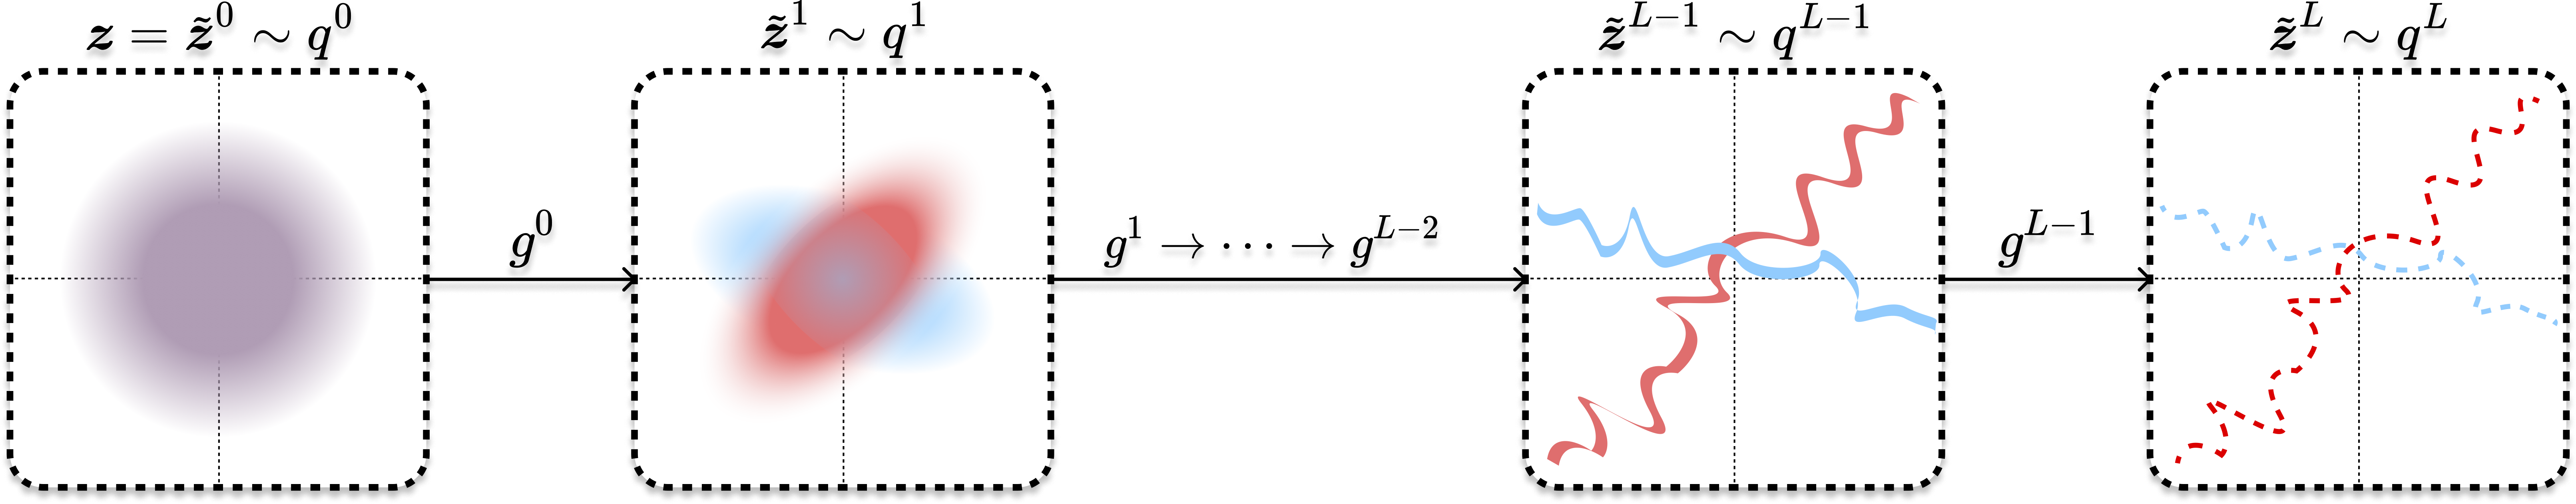
\includegraphics[width=\linewidth]{\toplevelprefix/chapters/chapter3/figs/diffusion_pipeline.png}
	\caption{一个迭代去噪过程的图示,从一个各向同性的高斯分布开始,收敛到一个任意的数据分布。}
	\label{fig:diffusion-chapter3}
\end{figure}

\subsection{扩散和去噪过程} \label{sub:intro_diffusion_denoising}

我们首先想要找到一个程序,将一个给定的非常嘈杂的样本的熵降低,使其成为一个来自数据分布的低熵样本。在这里,我们描述一个可能的方法——众多方法中的一种,但也许是解决这个问题最自然的方式。首先,我们找到一种方法来\textit{逐渐增加}来自数据分布的现有样本的熵。然后,我们找到这个过程的\textit{近似逆过程}。但总的来说,增加熵的操作没有逆过程,因为来自原始分布的信息可能会被破坏。因此,我们将处理一个特殊情况,其中(1)增加熵的操作采用简单、可计算和可逆的形式;(2)我们可以获得数据分布的(参数化)编码,如上述两种方法中所暗示的。正如我们将看到的,上述两个因素将确保我们的方法是可行的。

我们将以可以说最简单的方式增加熵,即\textit{添加各向同性高斯噪声}。更准确地说,给定随机变量 \(\vx\),我们可以考虑\textit{随机过程} \((\vx_{t})_{t \in [0, T]}\),它逐渐向其添加噪声,即
\begin{equation}\label{eq:additive_gaussian_noise_model}
	\vx_{t} \doteq \vx + t\vg, \qquad \forall t \in [0, T],
\end{equation}
其中 \(T \in [0, \infty]\) 是一个时间范围,\(\vg \sim \dNorm(\vzero, \vI)\) 是独立于 \(\vx\) 抽取的。这个过程是\textit{扩散过程}的一个例子,之所以这样命名,是因为它随着时间的推移将概率质量散布到整个 \(\R^{D}\) 上,从而随时间增加熵。这个直觉在 \Cref{fig:ve_forward_density} 中得到了图形化的证实,并通过以下定理得到了严格的证实。
\begin{theorem}[简化版的 \Cref{thm:diffusion_entropy_increases}]
	假设 \((\vx_{t})_{t \in [0, T]}\) 遵循模型 \eqref{eq:additive_gaussian_noise_model}。对于任何 \(t \in (0, T]\),随机变量 \(\vx_{t}\) 的微分熵 \(h(\vx_{t}) > -\infty\)。此外,在 \(\vx\) 的某些技术条件下,
	\begin{equation}
		\odv*{h(\vx_{t})}{t} > 0, \qquad \forall t \in (0, T],
	\end{equation}
	表明加噪的 \(\vx\) 的熵随时间 \(t\) 增加。
\end{theorem}
证明是初等的,但相当长,所以我们将其推迟到 \Cref{sub:diffusion_entropy_increases}。这个结果的主要尚未说明的含义是,对于每个 \(t > 0\),\(h(\vx_{t}) > h(\vx)\)。要看到这一点,请注意,如果 \(h(\vx) = -\infty\),那么对于所有 \(t > 0\),\(h(\vx_{t}) > -\infty\),如果 \(h(\vx) > -\infty\),那么根据微积分基本定理,\(h(\vx_{t}) = h(\vx) + \int_{0}^{t}[\odv*{h(\vx_{s})}{s}]\odif{s} > h(\vx)\),所以在两种情况下,对于每个 \(t > 0\),都有 \(h(\vx_{t}) > h(\vx)\)。

\begin{figure}
	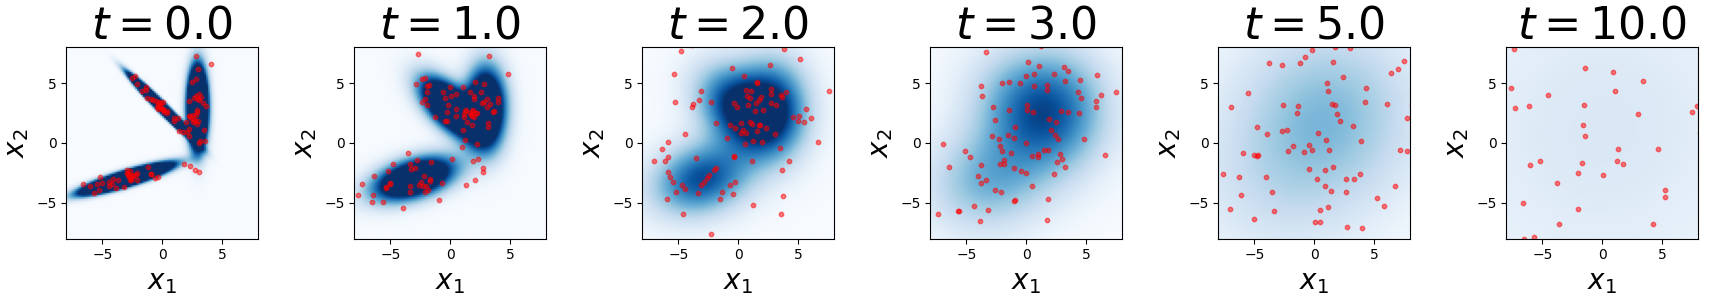
\includegraphics[width=\textwidth]{\toplevelprefix/chapters/chapter3/figs/ve_forward_diffusion_density.png}
	\caption{\small\textbf{扩散一个高斯混合模型。} 从左到右,我们观察到当 \(t\) 从 \(0\) 增长到 \(10\) 时密度的演变,以及一些代表性样本。每个区域根据其密度着色(\(0.0\) 是纯白色,\(> 0.01\) 是深蓝色,其他所有值映射到介于两者之间的某种蓝色调。)我们观察到,随着 \(t\) 的增加,概率质量变得不那么集中,这表明熵在增加。}
	\label{fig:ve_forward_density}
\end{figure}

加噪的逆操作被称为\textit{去噪}。这是信号处理和系统理论中一个经典且研究充分的课题,例如维纳滤波器和卡尔曼滤波器。\Cref{ch:classic} 中讨论的几个问题,如PCA、ICA和字典学习,都是去噪问题的具体实例。对于一个固定的 \(t\) 和加性高斯噪声模型 \eqref{eq:additive_gaussian_noise_model},去噪问题可以被表述为试图学习一个函数 \(\bar{\vx}^{\ast}(t, \cdot)\),该函数在给定 \(t\) 和 \(\vx_{t}\) 的情况下,形成对真实随机变量 \(\vx\) 的最佳可能近似(在期望意义上):
\begin{equation}\label{eq:denoising_loss}
	\bar{\vx}^{\ast}(t, \cdot) \in \argmin_{\bar{\vx}(t, \cdot)}\Ex_{\vx, \vx_{t}}\norm{\vx - \bar{\vx}(t, \vx_{t})}_{2}^{2}.
\end{equation}
当在所有可能的(平方可积)函数上优化 \(\bar{\vx}(t, \cdot)\) 时,这个问题的解是所谓的\textit{贝叶斯最优去噪器}:
\begin{equation}\label{eq:optimal_denoiser}
	\bar{\vx}^{\ast}(t, \vxi) \doteq \Ex[\vx \mid \vx_{t} = \vxi].
\end{equation}

这个表达式证明了符号 \(\bar{\vx}\) 的合理性,它意在计算一个条件期望(即条件均值或条件平均值)。简而言之,它试图从噪声输入中去除噪声,输出对(去噪后的)原始随机变量的最佳可能猜测(在期望和 \(\ell^{2}\)-距离的意义上)。

\begin{example}[从高斯混合模型中去噪高斯噪声]\label{example:denoising_gaussian_mixture}
	在这个例子中,我们计算一个极其重要的分布类别——高斯混合模型的贝叶斯最优去噪器。首先,让我们为分布固定参数:混合权重 \(\vpi \in \R^{K}\),成分均值 \(\{\vmu_{k}\}_{k = 1}^{K} \subseteq \R^{D}\),以及成分协方差 \(\{\vSigma_{k}\}_{k = 1}^{K} \subseteq \PSD(D)\),其中 \(\PSD(D)\) 是 \(D \times D\) 对称正半定矩阵的集合。现在,假设 \(\vx\) 是通过以下两步过程生成的:
	\begin{itemize}
		\item 首先,采样一个索引(或\textit{标签})\(y \in [K]\),使得 \(y = k\) 的概率为 \(\pi_{k}\)。
		\item 其次,从正态分布 \(\dNorm(\vmu_{y}, \vSigma_{y})\) 中采样 \(\vx\)。
	\end{itemize}
	那么 \(\vx\) 的分布为
	\begin{equation}
		\vx \sim \sum_{k = 1}^{K}\pi_{k}\dNorm(\vmu_{k}, \vSigma_{k}),
	\end{equation}
	所以
	\begin{equation}
		\vx_{t} = \vx + t\vg \sim \sum_{k = 1}^{K}\pi_{k}\dNorm(\vmu_{k}, \vSigma_{k} + t^{2}\vI).
	\end{equation}
	让我们定义 \(\phi(\vx ; \vmu, \vSigma)\) 为 \(\dNorm(\vmu, \vSigma)\) 在 \(\vx\) 处的概率密度。在这种表示法中,\(\vx_{t}\) 的密度是
	\begin{equation}
		p_{t}(\vx_{t}) = \sum_{k = 1}^{K}\pi_{k}\phi(\vx_{t} ; \vmu_{k}, \vSigma_{k} + t^{2}\vI).
	\end{equation}

	以 \(y\) 为条件,变量是联合高斯的:如果我们说 \(\vx = \vmu_{y} + \vSigma_{y}^{1/2}\vu\),其中 \((\cdot)^{1/2}\) 是矩阵平方根,\(\vu \sim \dNorm(\vzero, \vI)\) 独立于 \(y\)(和 \(\vg\)),那么我们有
	\begin{equation}
		\mat{\vx \\ \vx_{t}} = \mat{\vmu_{y} \\ \vmu_{y}} + \mat{\vSigma_{y}^{1/2} & \vzero \\ \vSigma_{y}^{1/2} & t\vI}\mat{\vu \\ \vg}.
	\end{equation}
	这表明 \(\vx\) 和 \(\vx_{t}\) 是联合高斯的(以 \(y\) 为条件),正如所声称的。因此我们可以写
	\begin{equation}
		\mat{\vx \\ \vx_{t}} \sim \dNorm\rp{\mat{\vmu_{y} \\ \vmu_{y}}, \mat{\vSigma_{y} & \vSigma_{y} \\ \vSigma_{y} & \vSigma_{y} + t^{2}\vI}}.
	\end{equation}
	因此,给定 \(\vx_{t}\) 时 \(\vx\) 的条件期望(即以 \(y\) 为条件的贝叶斯最优去噪器)是著名的
	(\Cref{exercise:conditional_gaussian})
	\begin{equation}
		\Ex[\vx \mid \vx_{t}, y] = \vmu_{y} + \vSigma_{y}(\vSigma_{y} + t^{2}\vI)^{-1}(\vx_{t} - \vmu_{y}).
	\end{equation}
	为了找到总的贝叶斯最优去噪器,我们使用迭代期望定律,得到
	\begin{align}
		\bar{\vx}^{\ast}(t, \vx_{t})
		&= \Ex[\vx \mid \vx_{t}] \\ 
		&= \Ex[\Ex[\vx \mid \vx_{t}, y] \mid \vx_{t}] \\ 
		&= \sum_{k = 1}^{K}\Pr[y = k \mid \vx_{t}]\Ex[\vx \mid \vx_{t}, y = k].
	\end{align}
	概率可以按如下方式处理。设 \(p_{t \mid y}\) 是以 \(y\) 的值为条件的 \(\vx_{t}\) 的概率密度。那么
	\begin{align}
		\Pr[y = k \mid \vx_{t}]
		&= \frac{p_{t \mid y}(\vx_{t} \mid k)\pi_{k}}{p_{t}(\vx_{t})} \\ 
		&= \frac{\pi_{k}\phi(\vx_{t} ; \vmu_{k}, \vSigma_{k}
		+ t^{2}\vI)}{\sum_{i = 1}^{K}\pi_{i}\phi(\vx_{t} ; \vmu_{i}, \vSigma_{i} + t^{2}\vI)}.
	\end{align}
	另一方面,条件期望如前所述:
	\begin{equation}
		\Ex[\vx \mid \vx_{t}, y = k] = \vmu_{k} + \vSigma_{k}(\vSigma_{k} + t^{2}\vI)^{-1}(\vx_{t} - \vmu_{k}).
	\end{equation}
	所以把这些放在一起,真正的贝叶斯最优去噪器是
	\begin{equation}\label{eq:gmm_bayes_optimal_denoiser}
		\bar{\vx}^{\ast}(t, \vx_{t}) = \sum_{k = 1}^{K}\frac{\pi_{k}\phi(\vx_{t}
		;\vmu_{k}, \vSigma_{k} + t^{2}\vI)}{\sum_{i = 1}^{K}\pi_{i}\phi(\vx_{t}
		;\vmu_{i}, \vSigma_{i} + t^{2}\vI)}\cdot\bp{\vmu_{k} + \vSigma_{k}(\vSigma_{k} + t^{2}\vI)^{-1}(\vx_{t} - \vmu_{k})}.
	\end{equation}
	这个例子特别重要,几个特例将在后面给我们带来重要的概念性洞察。现在,让我们尝试从最优去噪器 \eqref{eq:gmm_bayes_optimal_denoiser} 的函数形式中提取一些几何直觉。

	为了直观地理解 \eqref{eq:gmm_bayes_optimal_denoiser},让我们首先设 \(K = 1\)(即一个高斯分布),使得 \(\vx \sim \dNorm(\vmu, \vSigma)\)。然后让我们对角化 \(\vSigma = \vV\vLambda \vV^{\top}\)。那么贝叶斯最优去噪器是
	\begin{equation}
		\bar{\vx}^{\ast}(t, \vx_{t}) = \vmu + \vSigma(\vSigma + t^{2}\vI)^{-1}(\vx_{t} - \vmu) = \vmu + \vV\mat{\lambda_{1}/(\lambda_{1} + t^{2}) & & \\ & \ddots & \\ & & \lambda_{D}/(\lambda_{D} + t^{2})}\vV^{\top}(\vx_{t} - \vmu),
	\end{equation}
	其中 \(\lambda_{1}, \dots, \lambda_{D}\) 是 \(\vSigma\) 的特征值。我们可以观察到这个去噪器有三个步骤:
	\begin{itemize}
		\item 将输入 \(\vx_{t}\) 平移 \(\vmu\)。
		\item 在每个特征向量方向上,将(平移后的)输入 \(\vx_{t} - \vmu\) 收缩一个量 \(\lambda_{i}/(\lambda_{i} + t^{2})\)。如果平移后的输入是低秩的,并且 \(\vSigma\) 的某些特征值为零,这些方向会立即被去噪器收缩到 \(0\),确保收缩的输出同样是低秩的。
		\item 将输出平移回 \(\vmu\)。
	\end{itemize}
	很容易证明它将当前的 \(\vx_{t}\) 朝着均值 \(\vmu\) 收缩:
	\begin{equation}\label{eq:contraction}
		\norm{\bar{\vx}^{\ast}(t, \vx_{t}) - \vmu}_{2} \leq \norm{\vx_{t} - \vmu}_{2}.
	\end{equation}

	这是\textit{单个}高斯分布去噪器的几何解释。高斯混合模型 \eqref{eq:gmm_bayes_optimal_denoiser} 的整体去噪器使用 \(K\) 个这样的去噪器,通过后验概率 \(\Pr[y = k \mid \vx_{t}]\) 对它们的输出进行加权。如果高斯分布的均值分离得很好,这些后验概率在每个均值或聚类附近非常接近 \(0\) 或 \(1\)。在这种情况下,整体去噪器 \eqref{eq:gmm_bayes_optimal_denoiser} 具有与上述单个高斯去噪器相同的几何解释。

    乍一看,这样的收缩映射 \eqref{eq:contraction} 可能看起来类似于幂迭代法(参见 \Cref{subsec:power iterations})。然而,这两者在根本上是不同的。幂迭代法实现的是朝向一个子空间的收缩映射——即由第一主成分张成的子空间。相比之下,\eqref{eq:contraction} 中的迭代收敛到底层分布的均值 \(\vmu\),这是一个单点。
\end{example}

\begin{figure}
	\centering 
	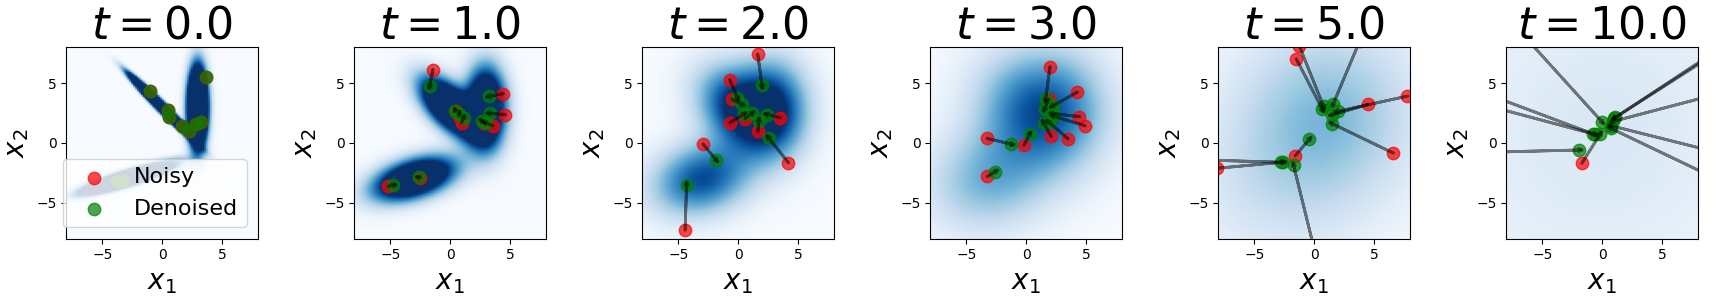
\includegraphics[width=\textwidth]{\toplevelprefix/chapters/chapter3/figs/ve_forward_diffusion_denoising.png}\vspace{-0.15in}
	\caption{\small \textbf{高斯混合模型的贝叶斯最优去噪器和分数。} 在与 \Cref{fig:ve_forward_density} 相同的设置下,我们通过绘制 \(\vx_{t}\)(红色)和 \(\bar{\vx}^{\ast}(t, \vx_{t})\)(绿色)来展示贝叶斯最优去噪器 \(\bar{\vx}^{\ast}\) 的效果,其中 \(t\) 和 \(\vx_{t}\) 为某个选定值。根据特威迪公式 \Cref{thm:tweedie},它们之间的残差与所谓的(Hyv\"arinen)分数 \(\nabla_{\vx_{t}}\log p_{t}(\vx_{t})\) 成正比。我们可以看到,分数指向 \(\vx_{t}\) 分布的众数。}
	\label{fig:ve_forward_denoising}
\end{figure}

直观上,正如我们从 \Cref{example:denoising_gaussian_mixture} 中可以看到的,贝叶斯最优去噪器 \(\bar{\vx}^{\ast}(t, \cdot)\) 应该将其输入 \(\vx_{t}\) 移向 \(\vx\) 分布的众数。事实证明,实际上,我们可以通过证明贝叶斯最优去噪器在 \(\vx_{t}\) 的(对数)密度上\textit{进行梯度上升步骤}来量化这一点,我们(回顾一下)将其表示为 \(p_{t}\)。也就是说,遵循去噪器意味着从输入迭代移动到这个(扰动后的)分布中概率更高的区域。对于小的 \(t\),扰动很小,因此我们最初的直觉(几乎)完全正确。这个情景在 \Cref{fig:ve_forward_denoising} 中可视化,并被严格地表述为特威迪公式 \cite{Robbins1956AnEB}。
\begin{theorem}[特威迪公式]\label{thm:tweedie}
	假设 \((\vx_{t})_{t \in [0, T]}\) 遵循 \eqref{eq:additive_gaussian_noise_model}。设 \(p_{t}\) 是 \(\vx_{t}\) 的密度(如前所述)。那么
	\begin{equation}\label{eq:tweedie}
		\Ex[\vx \mid \vx_{t}] = \vx_{t} + t^{2}\nabla_{\vx_{t}} \log p_{t}(\vx_{t}).
	\end{equation}
\end{theorem}
\begin{proof}
	为了证明,我们假设 \(\vx\) 有一个密度(尽管定理在没有这个假设的情况下也成立),并称这个密度为 \(p\)。设 \(p_{0 \mid t}\) 和 \(p_{t \mid 0}\) 分别是给定 \(\vx_{t}\) 时 \(\vx = \vx_{0}\) 的条件密度和给定 \(\vx\) 时 \(\vx_{t}\) 的条件密度。设 \(\phi(\vx ; \vmu, \vSigma)\) 是在 \(\vx\) 处评估的 \(\dNorm(\vmu, \vSigma)\) 的密度,因此 \(p_{t \mid 0}(\vx_{t} \mid \vx) = \phi(\vx_{t} ; \vx, t^{2}\vI)\)。那么一个简单的计算给出
	\begin{align}
		\nabla_{\vx_{t}} \log p_{t}(\vx_{t})
		&= \frac{\nabla_{\vx_{t}}p_{t}(\vx_{t})}{p_{t}(\vx_{t})} \\
		&= \frac{1}{p_{t}(\vx_{t})}\nabla_{\vx_{t}}\int_{\R^{D}}p(\vx)p_{t \mid 0}(\vx_{t} \mid \vx)\odif{\vx} \\
		&=
		\frac{1}{p_{t}(\vx_{t})}\nabla_{\vx_{t}}\int_{\R^{D}}p(\vx)\phi(\vx_{t}
		;\vx, t^{2}\vI)\odif{\vx} \\
		&=
		\frac{1}{p_{t}(\vx_{t})}\int_{\R^{D}}p(\vx)[\nabla_{\vx_{t}}\phi(\vx_{t}
		;\vx, t^{2}\vI)]\odif{\vx} \\
		&= \frac{1}{p_{t}(\vx_{t})}\int_{\R^{D}}p(\vx)\phi(\vx_{t} ; \vx, t^{2}\vI)\bs{-\frac{\vx_{t} - \vx}{t^{2}}}\odif{\vx} \\
		&= \frac{1}{t^{2}p_{t}(\vx_{t})}\int_{\R^{D}}p(\vx)\phi(\vx_{t} ; \vx, t^{2}\vI)[\vx - \vx_{t}]\odif{\vx} \\
		&= \frac{1}{t^{2}p_{t}(\vx_{t})}\int_{\R^{D}}p(\vx)\phi(\vx_{t} ; \vx,
		t^{2}\vI)\vx \odif{\vx}
		- \frac{\vx_{t}}{t^{2}p_{t}(\vx_{t})}\int_{\R^{D}}p(\vx)\phi(\vx_{t} ; \vx, t^{2}\vI)\odif{\vx} \\
		&= \frac{1}{t^{2}p_{t}(\vx_{t})}\int_{\R^{D}}p(\vx)p_{t \mid 0}(\vx_{t} \mid \vx)\vx \odif{\vx} - \frac{\vx_{t}}{t^{2}p_{t}(\vx_{t})}p_{t}(\vx_{t}) \\
		&= \frac{1}{t^{2}p_{t}(\vx_{t})}\int_{\R^{D}}p_{t}(\vx_{t})p_{0 \mid t}(\vx \mid \vx_{t})\vx \odif{\vx} - \frac{\vx_{t}}{t^{2}p_{t}(\vx_{t})}p_{t}(\vx_{t}) \\
		&= \frac{1}{t^{2}}\int_{\R^{D}}p_{0 \mid t}(\vx \mid \vx_{t})\vx \odif{\vx} - \frac{\vx_{t}}{t^{2}} \\
		&= \frac{1}{t^{2}}\Ex[\vx \mid \vx_{t}] - \frac{\vx_{t}}{t^{2}} \\
		&= \frac{\Ex[\vx \mid \vx_{t}] - \vx_{t}}{t^{2}}.
	\end{align}
	简单地重新排列上述等式即可证明该定理。
\end{proof}
这个结果在去噪和优化之间建立了联系:贝叶斯最优去噪器在扰动后的数据密度 \(p_{t}\) 上进行单步梯度上升,并且随着对数据分布的扰动变小,步长自适应地变小(即,采取更精确的步骤)。数量 \(\nabla_{\vx_{t}}\log p_{t}(\vx_{t})\) 被称为\textit{(Hyv\"arinen)分数},并经常出现在关于去噪等的讨论中;它首次出现在 Aapo Hyv\"arinen 的一篇关于 ICA 的论文中 \cite{hyvarinen05a}。

类似于在实践中当从远离最优点初始化时,一步梯度下降几乎不足以最小化一个目标函数,当 \(t\) 很大时,贝叶斯最优去噪器 \(\bar{\vx}^{\ast}(t, \cdot)\) 的输出几乎不包含在数据分布的高概率区域内,\textit{特别是}当数据具有低维结构时。我们在下面的例子中明确说明了这一点。
\begin{example}[去噪一个两点混合分布]\label{example:denoising_twopoints}
	设 \(x\) 在两点集 \(\{-1, +1\}\) 上均匀分布,并设 \((\vx_{t})_{t \in [0, T]}\) 遵循 \eqref{eq:additive_gaussian_noise_model}。这正是一个退化的高斯混合模型,其先验概率等于 \(\frac{1}{2}\),均值为 \(\{-1, +1\}\),协方差都等于 \(0\)。对于一个固定的 \(t > 0\),我们可以使用 \eqref{eq:gmm_bayes_optimal_denoiser} 中贝叶斯最优去噪器的计算来获得(证明作为练习)
	\begin{equation}
		\bar{x}^{\ast}(t, x_{t}) = \frac{\phi(x_{t} ; +1, t^{2}) - \phi(x_{t}
		; -1, t^{2})}{\phi(x_{t} ; 1, t^{2}) + \phi(x_{t} ; -1, t^{2})} = \tanh\rp{-\frac{x_{t}}{t^{2}}}.
	\end{equation}
	对于接近 \(0\) 的 \(t\),对于几乎所有的输入 \(\bar{x}^{\ast}(t, x_{t})\),这个量都接近 \(\{-1, +1\}\)。然而,对于大的 \(t\),这个量不一定甚至近似地在 \(x\) 的原始支撑集 \(\{-1, +1\}\) 中。特别是,对于 \(x_{t} \approx 0\),有 \(\bar{x}^{\ast}(t, x_{t}) \approx 0\),它完全位于两个可能的点之间。因此,\(\bar{x}^{\ast}\) \textit{不会输出“真实的” \(x\)}。或者更数学地说,\(\bar{x}(t, x_{t})\) 的分布与 \(x\) 的分布非常不同。
\end{example}

因此,如果我们想对非常嘈杂的样本 \(\vx_{T}\)(其中——回想一下——\(T\) 是最大时间)进行去噪,我们不能只使用去噪器\textit{一次}。相反,我们必须多次使用去噪器,类似于使用\textit{衰减步长}的梯度下降,以收敛到一个平稳点 \(\hat{\vx}\)。也就是说,我们应该使用去噪器从 \(\vx_{T}\) 到 \(\hat{\vx}_{T - \delta}\)(它近似于 \(\vx_{T - \delta}\)),然后从 \(\hat{\vx}_{T - \delta}\) 到 \(\hat{\vx}_{T - 2\delta}\),等等,一直从 \(\hat{\vx}_{\delta}\) 到 \(\hat{\vx} = \hat{\vx}_{0}\)。每次我们进行去噪步骤时,去噪器的作用变得更像是在原始(对数)密度上进行梯度步骤。

更正式地,我们将 \([0, T]\) 均匀离散化为 \(L + 1\) 个时间步 \(0 = t_{0} < t_{1} < \cdots < t_{L} = T\),即
\begin{equation}
	t_{\ell} = \frac{\ell}{L}T, \qquad \ell \in \{0, 1, \dots, L\}.
\end{equation}
然后对于每个 \(\ell \in [L] = \{1, 2, \dots, L\}\),从 \(\ell = L\) 到 \(\ell = 1\),我们可以运行迭代
\begin{align}
	\hat{\vx}_{t_{\ell - 1}}
	&= \Ex[\vx_{t_{\ell - 1}} \mid \vx_{t_{\ell}} = \hat{\vx}_{t_{\ell}}] \\
	&= \Ex[\vx + t_{\ell - 1}\vg \mid \vx_{t_{\ell}} = \hat{\vx}_{t_{\ell}}] \\
	&= \Ex\rs{\vx + t_{\ell - 1}\cdot\frac{\vx_{t_{\ell}} - \vx}{t_{\ell}} \given \vx_{t_{\ell}} = \hat{\vx}_{t_{\ell}}} \\
	&= \frac{t_{\ell - 1}}{t_{\ell}}\hat{\vx}_{t_{\ell}} + \bp{1 - \frac{t_{\ell - 1}}{t_{\ell}}}\Ex[\vx \mid \vx_{t_{\ell}} = \hat{\vx}_{t_{\ell}}] \\
	&= \bp{1 - \frac{1}{\ell}}\cdot\hat{\vx}_{t_{\ell}} + \frac{1}{\ell}\cdot\bar{\vx}^{\ast}(t_{\ell}, \hat{\vx}_{t_{\ell}}).
\end{align}
这个迭代的效果如下。在迭代开始时,当 \(\ell\) 很大时,我们几乎不相信去噪器的输出,而主要保留当前的迭代值。这是有道理的,因为去噪器可能有很大的方差(参见 \Cref{example:denoising_twopoints})。当 \(\ell\) 很小时,去噪器将“锁定”到数据分布的众数,因为去噪步骤基本上是在真实分布的对数密度上进行梯度步骤,我们可以相信它不会产生不合理的样本,所以去噪步骤主要涉及去噪器的输出。在 \(\ell = 1\) 时,我们甚至扔掉当前的迭代值,只保留去噪器的输出。

\begin{figure}[t]
	\centering
	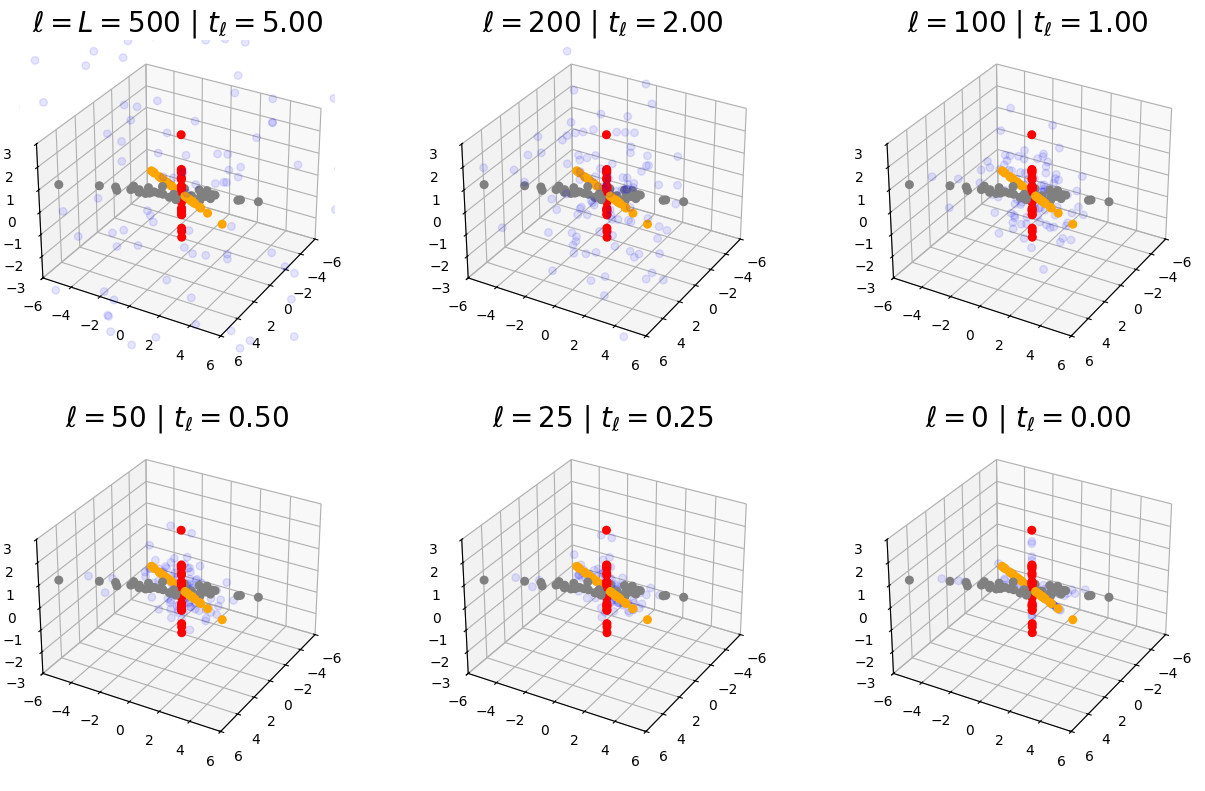
\includegraphics[width=\textwidth]{\toplevelprefix/chapters/chapter3/figs/ve_gmm_denoising.png}
	\caption{\small\textbf{去噪一个低秩高斯混合模型。} 每个图表示来自真实数据分布的样本(灰色、橙色、红色)和正在经历去噪过程 \eqref{eq:denoising-iteration-basic} 的样本(浅蓝色)。左上角,过程刚刚开始,噪声非常大。随着过程的继续,噪声被进一步推向低秩数据分布的支撑集。最后,在右下角,生成的样本与数据的支撑集完美对齐,看起来非常像从低秩高斯混合模型中抽取的样本。}
	\label{fig:ve_gmm_denoising}
\end{figure}

以上是我们期望去噪过程收敛的直觉。我们在 \(\R^{3}\) 中可视化了收敛过程,见 \Cref{fig:ve_gmm_denoising}。我们稍后将为收敛建立一些严格的结果。现在,回想一下我们想要建立一个降低熵的过程。虽然我们通过逆转一个增加熵的过程以一种迂回的方式做到了这一点,但现在是时候付出代价,确认我们的迭代去噪过程确实降低了熵。

\begin{theorem}[简化版的 \Cref{thm:conditioning_reduces_entropy}]
	假设 \((\vx_{t})_{t \in [0, T]}\) 遵循 \eqref{eq:additive_gaussian_noise_model}。那么,在 \(\vx\) 的某些技术条件下,对于每个 \(s < t\) 且 \(s, t \in (0, T]\),
	\begin{equation}
		h(\Ex[\vx_{s} \mid \vx_{t}]) < h(\vx_{t}).
	\end{equation}
\end{theorem}
该定理的完整陈述及其证明需要一些技术性,因此推迟到 \Cref{sub:denoising_entropy_decreases}。

我们在这里讨论的最后一件事是,很多时候,我们\textit{无法计算}任何 \(t\) 的 \(\bar{\vx}^{\ast}(t, \cdot)\),因为我们没有分布 \(p_{t}\)。但是我们可以尝试\textit{从数据中学习一个}。回想一下,去噪器 \(\bar{\vx}^{\ast}\) 在 \eqref{eq:denoising_loss} 中被定义为最小化均方误差 \(\Ex\norm{\bar{\vx}(t, \vx_{t}) - \vx}_{2}^{2}\)。我们可以使用这个均方误差作为损失或目标函数来学习去噪器。例如,我们可以用一个神经网络来参数化 \(\bar{\vx}(t, \cdot)\),写作 \(\bar{\vx}_{\theta}(t, \cdot)\),并在参数空间 \(\Theta\) 上优化损失:
\begin{equation}
	\min_{\theta \in \Theta}\Ex_{\vx, \vx_{t}}\norm{\bar{\vx}_{\theta}(t, \vx_{t}) - \vx}_{2}^{2}.
\end{equation}
这个优化问题的解,通过梯度下降或类似算法实现,将给我们一个 \(\bar{\vx}_{\theta^{\ast}}(t, \cdot)\),它是 \(\bar{\vx}^{\ast}(t, \cdot)\) 的一个很好的近似(至少如果训练有效的话),我们将用它作为我们的去噪器。

这个神经网络 \(\bar{\vx}_{\theta^{\ast}}(t, \cdot)\) 的一个好架构是什么?为了回答这个问题,我们将研究一个普遍存在的案例,即\textit{高斯混合模型},我们在 \Cref{example:denoising_gaussian_mixture} 中计算了它的去噪器。这个模型是相关的,因为它可以近似许多类型的分布:特别是,给定一个 \(\vx\) 的分布,存在一个可以任意好地近似它的高斯混合模型。因此,在高斯混合模型的去噪器类别中进行优化可以给我们一些接近真实数据分布的最优去噪器的东西。

在我们的案例中,我们假设 \(\vx\) 是低维的,这粗略地转化为 \(\vx\) \textit{近似地}根据一个\textit{低秩高斯混合模型}分布的要求。形式上,我们写
\begin{equation}\label{eq:MoG1}
	\vx \sim \frac{1}{K}\sum_{k = 1}^{K}\dNorm(\vzero, \vU_{k}\vU_{k}^{\top})
\end{equation}
其中 \(\vU_{k} \in \O(D, P) \subseteq \R^{D \times P}\) 是一个正交矩阵。那么在 \eqref{eq:additive_gaussian_noise_model} 下的最优去噪器是(来自 \Cref{example:denoising_gaussian_mixture})
\begin{equation}
	\bar{\vx}^{\ast}(t, \vx_{t}) = \sum_{k = 1}^{K}\frac{\phi(\vx_{t} ; \vzero,
	\vU_{k}\vU_{k}^{\top} + t^{2}\vI)}{\sum_{i = 1}^{K}\phi(\vx_{t} ; \vzero, \vU_{i}\vU_{i}^{\top} + t^{2}\vI)}\cdot\bp{\vU_{k}\vU_{k}^{\top}(\vU_{k}\vU_{k}^{\top} + t^{2}\vI)^{-1}\vx_{t}}.
\end{equation}
注意到在计算 \(\phi\) 的内部和外部,我们都计算了逆矩阵 \((\vU_{k}\vU_{k}^{\top} + t^{2}\vI)^{-1}\)。这是一个满秩矩阵 \(t^{2}\vI\) 的低秩扰动,因此很适合通过\textit{Sherman-Morrison-Woodbury 恒等式}进行简化,即对于矩阵 \(\vA, \vC, \vU, \vV\),使得 \(\vA\) 和 \(\vC\) 是可逆的,
\begin{equation}\label{eq:sherman_morrison_woodbury}
	(\vA + \vU\vC\vV)^{-1} = \vA^{-1} - \vA^{-1}\vU(\vC^{-1} + \vV\vA^{-1}\vU)^{-1}\vV\vA^{-1}.
\end{equation}
我们在 \Cref{exercise:sherman_morrison_woodbury_identity} 中证明这个恒等式。现在我们应用这个恒等式,令 \(\vA = t^{2}\vI\),\(\vU = \vU_{k}\),\(\vV = \vU_{k}^{\top}\),和 \(\vC = \vI\),得到
\begin{align}
	(\vU_{k}\vU_{k}^{\top} + t^{2}\vI)^{-1} 
	&= \frac{1}{t^{2}}\vI - \frac{1}{t^{4}}\vU_{k}\bp{\vI + \frac{1}{t^{2}}\vU_{k}^{\top}\vU_{k}}^{-1}\vU_{k}^{\top} \\
	&= \frac{1}{t^{2}}\vI - \frac{1}{t^{4}\bp{1 + \frac{1}{t^{2}}}}\vU_{k}\vU_{k}^{\top} \\
	&= \frac{1}{t^{2}}\bp{\vI - \frac{1}{1 + t^{2}}\vU_{k}\vU_{k}^{\top}}.
\end{align}
然后我们可以如下计算后验概率。注意因为 \(\vU_{k}\) 都是正交的,所以对于每个 \(k\),\(\det(\vU_{k}\vU_{k}^{\top} + t^{2}\vI)\) 都是相同的。所以
\begin{align}
	\frac{\phi(\vx_{t} ; \vzero, \vU_{k}\vU_{k}^{\top} + t^{2}\vI)}{\sum_{i
	= 1}^{K}\phi(\vx_{t} ; \vzero, \vU_{i}\vU_{i}^{\top} + t^{2}\vI)} 
	&= \frac{\exp\rp{-\frac{1}{2}\vx_{t}^{\top}(\vU_{k}\vU_{k}^{\top} + t^{2}\vI)^{-1}\vx_{t}}}{\sum_{i = 1}^{K}\exp\rp{-\frac{1}{2}\vx_{t}^{\top}(\vU_{i}\vU_{i}^{\top} + t^{2}\vI)^{-1}\vx_{t}}} \\
	&= \frac{\exp\rp{-\frac{1}{2t^{2}}\vx_{t}^{\top}\bp{\vI - \frac{1}{1 + t^{2}}\vU_{k}\vU_{k}^{\top}}\vx_{t}}}{\sum_{i = 1}^{K}\exp\rp{-\frac{1}{2t^{2}}\vx_{t}^{\top}\bp{\vI - \frac{1}{1 + t^{2}}\vU_{i}\vU_{i}^{\top}}\vx_{t}}} \\
	&= \frac{\exp\rp{-\frac{1}{2t^{2}}\norm{\vx_{t}}_{2}^{2} + \frac{1}{2t^{2}(1 + t^{2})}\norm{\vU_{k}^{\top}\vx_{t}}_{2}^{2}}}{\sum_{i = 1}^{K}\exp\rp{-\frac{1}{2t^{2}}\norm{\vx_{t}}_{2}^{2} + \frac{1}{2t^{2}(1 + t^{2})}\norm{\vU_{i}^{\top}\vx_{t}}_{2}^{2}}} \\
	&= \frac{\exp\rp{-\frac{1}{2t^{2}}\norm{\vx_{t}}_{2}^{2}}\exp\rp{\frac{1}{2t^{2}(1 + t^{2})}\norm{\vU_{k}^{\top}\vx_{t}}_{2}^{2}}}{\exp\rp{-\frac{1}{2t^{2}}\norm{\vx_{t}}_{2}^{2}}\sum_{i = 1}^{K}\exp\rp{\frac{1}{2t^{2}(1 + t^{2})}\norm{\vU_{i}^{\top}\vx_{t}}_{2}^{2}}} \\
	&= \frac{\exp\rp{\frac{1}{2t^{2}(1 + t^{2})}\norm{\vU_{k}^{\top}\vx_{t}}_{2}^{2}}}{\sum_{i = 1}^{K}\exp\rp{\frac{1}{2t^{2}(1 + t^{2})}\norm{\vU_{i}^{\top}\vx_{t}}_{2}^{2}}}.
\end{align}
这是一个由 \(\vx_{t}\) 在每个子空间上的投影(由 \(\norm{\vU_{i}^{\top}\vx_{t}}_{2}\) 衡量)加权的 softmax 操作(由温度 \(2t^{2}(1 + t^{2})\) 调节)。同时,成分去噪器可以写作
\begin{align}
	\vU_{k}\vU_{k}^{\top}(\vU_{k}\vU_{k}^{\top} + t^{2}\vI)^{-1}\vx_{t} 
	&= \frac{1}{t^{2}}\vU_{k}\vU_{k}^{\top}\bp{\vI - \frac{1}{1 + t^{2}}\vU_{k}\vU_{k}^{\top}}\vx_{t} \\
	&= \frac{1}{t^{2}}\bp{1 - \frac{1}{1 + t^{2}}}\vU_{k}\vU_{k}^{\top}\vx_{t} \\
	&= \frac{1}{1 + t^{2}}\vU_{k}\vU_{k}^{\top}\vx_{t}.
\end{align}
将这些放在一起,我们有
\begin{equation}\label{eq:gmm_lowrank_denoiser}
	\bar{\vx}^{\ast}(t, \vx_{t}) = \frac{1}{1 + t^{2}}\sum_{k = 1}^{K}\frac{\exp\rp{\frac{1}{2t^{2}(1 + t^{2})}\norm{\vU_{k}^{\top}\vx_{t}}_{2}^{2}}}{\sum_{i = 1}^{K}\exp\rp{\frac{1}{2t^{2}(1 + t^{2})}\norm{\vU_{i}^{\top}\vx_{t}}_{2}^{2}}}\vU_{k}\vU_{k}^{\top}\vx_{t},
\end{equation}
即,将 \(\vx_{t}\) 投影到 \(K\) 个子空间中的每一个上,并由一个关于 \(\vx_{t}\) 的二次函数的 soft-max 操作加权。这种函数形式类似于 Transformer 架构中的\textit{注意力机制}!正如我们将在 \Cref{ch:representation} 中看到的,这绝非巧合;去噪和有损压缩(将在 \Cref{sec:lossy_compression} 中介绍)之间的深层联系使得 Transformer 去噪器在实践中如此有效。因此,总的来说,我们的高斯混合模型理论为使用类 Transformer 神经网络进行去噪提供了动机。

\begin{remark}
{\bf 去噪分布与概率PCA之间的联系。} 在这里,我们希望将去噪低维分布与概率PCA(有关概率PCA的更多细节,请参见 \Cref{subsec:probabilistic PCA})联系起来。假设我们在 \eqref{eq:MoG1} 中考虑 $K=1$,即 $\vx \sim \dNorm(\vzero, \vU\vU^{\top})$,其中 \(\vU \in \O(D, P) \subseteq \R^{D \times P}\) 是一个正交矩阵。根据 \eqref{eq:gmm_lowrank_denoiser},贝叶斯最优去噪器是
\begin{align}
    \bar{\vx}^{\ast}(t, \vx_{t}) = \frac{1}{1 + t^{2}} \vU\vU^\top\vx_t. 
\end{align}
为了学习这个贝叶斯最优去噪器,我们可以相应地将去噪算子 $\bar{\vx}(t,\vx_t)$ 参数化如下:
\begin{align}
    \bar{\vx}(t,\vx_t) = \frac{1}{1 + t^{2}} \vV\vV^\top\vx_t,
\end{align}
其中 $\vV \in \O(D, P)$ 是可学习的参数。将此代入训练损失 \eqref{eq:denoising_loss} 得到
\begin{equation}\label{eq:training loss PCA}
	  \min_{\vV \in \O(D, P)}\Ex_{\vx, \vx_{t}}\left\|\vx - \frac{1}{1 + t^{2}} \vV\vV^\top\vx_t\right\|_{2}^{2} = \Ex_{\vx, \vg}\left\|\vx - \frac{1}{1 + t^{2}} \vV\vV^\top(\vx + t\vg)\right\|_{2}^{2},
\end{equation}
其中等式是由于 \eqref{eq:additive_gaussian_noise_model}。以 $\vx$ 为条件,我们计算
\begin{align}
    & \Ex_{\vg}\left\|\vx - \frac{1}{1 + t^{2}} \vV\vV^\top(\vx + t\vg)\right\|_{2}^{2} \\
    = & \left\|\vx - \frac{1}{1 + t^{2}} \vV\vV^\top \vx\right\|_{2}^{2} - \frac{t}{1+t^2}\Ex_{\vg} \left\langle \vx - \frac{1}{1 + t^{2}} \vV\vV^\top \vx,  \vV\vV^\top\vg \right\rangle + \frac{t^2}{(1+t^2)^2} \Ex_{\vg}\left\| \vV\vV^\top \vg \right\|_2^2 \\
    = & \left\|\vx - \frac{1}{1 + t^{2}} \vV\vV^\top \vx\right\|_{2}^{2} + \frac{t^2P}{(1+t^2)^2} 
\end{align}
其中第二个等式是由于 \(\vg \sim \dNorm(\vzero, \vI)\) 和 $ \Ex_{\vg}\left\| \vV\vV^\top \vg \right\|_2^2 = \Ex_{\vg}\left\|\vV^\top \vg \right\|_2^2 = P$(因为 $\vV \in \O(D, P)$)。因此,问题 \eqref{eq:training loss PCA} 等价于
\begin{align}
    \min_{\vV \in \O(D, P)}\Ex_{\vx} \left\|\vx - \frac{1}{1 + t^{2}} \vV\vV^\top \vx\right\|_{2}^{2} = \Ex_{\vx} \|\vx\|_2^2 + \left( \frac{1}{(1+t^2)^2} - \frac{2}{1+t^2} \right) \Ex_{\vx}\|\vV^\top \vx\|_2^2.
\end{align}
这进一步等价于
\begin{align}
    \max_{\vV \in \O(D, P)} \Ex_{\vx}\|\vV^\top \vx\|_2^2,
\end{align}
这本质上是问题 \eqref{eq:PPCA}。
\end{remark}

总的来说,学习到的去噪器构成了给定数据的一种(隐式参数化)编码方案,因为它可以用于去噪/投影到数据分布上。训练去噪器等同于寻找一个更好的编码方案,这部分满足了 \Cref{sub:min_entropy} 末尾的期望之一(\textit{第二个})。接下来,我们将讨论如何满足另一个(\textit{第一个})。


\subsection{通过迭代去噪学习和采样分布}\label{sub:sampling_denoising}

回想一下,在 \Cref{sub:min_entropy} 的末尾,我们讨论了追求具有低维结构的分布的一对期望。第一个期望是从一个正态分布开始,比如具有高熵,然后逐渐降低其熵,直到达到数据的分布。我们将这个过程称为\textit{采样},因为我们正在生成新的样本。现在是我们讨论如何用我们已经建立的工具包来做到这一点的时候了。

我们知道如何对非常嘈杂的样本 \(\vx_{T}\) 进行去噪,以获得与目标随机变量 \(\vx\) 具有相似分布的近似 \(\hat{\vx}\)。但是期望说,要进行采样,我们希望从一个\textit{不受} \(\vx\) 分布影响的模板分布开始,并使用去噪器引导迭代走向 \(\vx\) 的分布。我们该如何做到这一点?一种方法的动机如下:
\begin{equation}\label{eq:ve_converge_to_large_gaussian}
	\frac{\vx_{T}}{T} = \frac{\vx + T\vg}{T} = \frac{\vx}{T} + \vg \to \vg \sim \dNorm(\vzero, \vI).
\end{equation}
因此,\(\vx_{T} \approx \dNorm(\vzero, T^{2}\vI)\)。这个近似对于几乎所有实际分布都相当好,并在 \Cref{fig:xT_vs_noise} 中进行了可视化。
\begin{figure}
	\centering 
	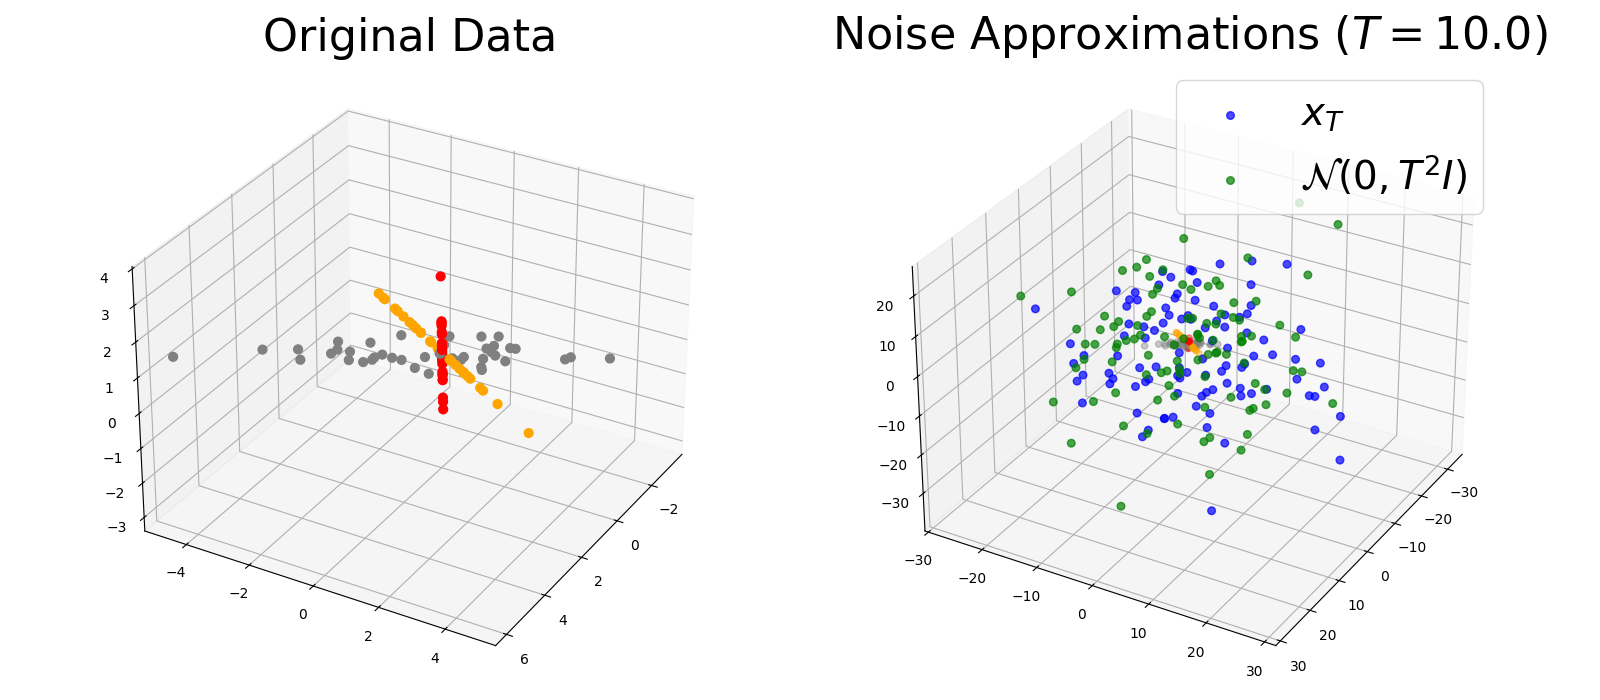
\includegraphics[width=0.75\textwidth]{\toplevelprefix/chapters/chapter3/figs/xT_vs_noise.png}
	\caption{\small\textbf{可视化 \(\vx_{T}\) 与 \(\dNorm(\vzero, T^{2}\vI)\)。} \textit{左图:} 高斯混合模型数据 \(\vx\) 的图。 \textit{右图:} \(\vx\) 以及 \(\vx_{T}\) 和一个独立的 \(\dNorm(\vzero, T^{2}\vI)\) 样本的图,其中 \(T = 10\)。在右图中,\(\vx\) 的颜色与左图相同:然而,来自 \(\vx_{T}\) 和 \(\dNorm(\vzero, T^{2}\vI)\) 的样本平均比来自 \(\vx\) 的样本大得多,因此由于缩放的原因,它看起来小得多。尽管有这种大的放大,我们清楚地观察到 \(\vx_{T}\) 和 \(\dNorm(\vzero, T^{2}\vI)\) 分布的相似性。}
	\label{fig:xT_vs_noise}
\end{figure}

所以,将 \([0, T]\) 均匀离散化为 \(0 = t_{0} < t_{1} < \cdots < t_{L} = T\),使用 \(t_{\ell} = T\ell / L\)(如上一节),一种从纯噪声中采样的方法是:
\begin{itemize}
	\item 采样 \(\hat{\vx}_{T} \sim \dNorm(\vzero, T^{2}\vI)\)(独立同分布于其他所有变量)
	\item 运行去噪迭代,如 \Cref{sub:intro_diffusion_denoising} 中所述,即
		\begin{equation}\label{eq:denoising-iteration-basic}
		\hat{\vx}_{t_{\ell - 1}} = \bp{1 - \frac{1}{\ell}}\cdot\hat{\vx}_{t_{\ell}} + \frac{1}{\ell}\cdot\bar{\vx}^{\ast}(t_{\ell}, \hat{\vx}_{t_{\ell}}).
	\end{equation}
	\item 输出 \(\hat{\vx} = \hat{\vx}_{0}\)。
\end{itemize}
这在概念上就是\textit{扩散模型}背后的全部内容,它根据第一个期望将噪声转化为数据样本。然而,在我们得到能够从像图像这样的真实数据分布中采样,并且在实际资源限制下可行的模型之前,还有几个步骤需要走。接下来,我们将介绍并论证几个这样的步骤。

\paragraph{步骤 1:不同的离散化方法。} 我们做的第一步是基于以下观点:\textit{我们不需要在大的 \(t\) 值上花费那么多的去噪迭代}。如果我们看 \Cref{fig:ve_gmm_denoising},我们观察到在采样过程的 \(500\) 次迭代中,前 \(200\) 或 \(300\) 次迭代只是将噪声整体收缩到数据分布,然后剩余的迭代才将样本推向一个子空间。在固定的迭代次数 \(L\) 下,这表明我们应该在 \(t = 0\) 附近花费更多的时间步 \(t_{\ell}\),而不是在 \(t = T\) 附近。因此,在采样(和训练)期间,我们可以使用 \([0, T]\) 的另一种离散化方法,例如\textit{指数离散化}:
\begin{equation}\label{eq:denoising_exponential_discretization}
	t_{\ell} = C_{1}(e^{C_{2}\ell} - 1), \qquad \forall \ell \in \{0, 1, \dots, L\}
\end{equation}
其中 \(C_{1}, C_{2} > 0\) 是可以在实践中调整以获得最佳性能的常数;理论分析通常也会指定这样的最优常数。然后去噪/采样迭代变为
\begin{equation}\label{eq:denoising_iteration}
	\hat{\vx}_{t_{\ell - 1}} \doteq \frac{t_{\ell - 1}}{t_{\ell}}\hat{\vx}_{t_{\ell}} + \bp{1 - \frac{t_{\ell - 1}}{t_{\ell}}}\bar{\vx}^{\ast}(t_{\ell}, \hat{\vx}_{t_{\ell}}),
\end{equation}
同样,\(\hat{\vx}_{t_{L}} \sim \dNorm(\vzero, t_{L}^{2}\vI)\)。

\paragraph{步骤 2:不同的噪声模型。} 第二步是考虑与 \eqref{eq:additive_gaussian_noise_model} 略有不同的模型。这样做的基本动机如下。在实践中,噪声分布 \(\dNorm(\vzero, t_{L}^{2}\vI)\) 在高维空间中对真实协方差的估计变得越来越差,即 \eqref{eq:ve_converge_to_large_gaussian} 成为一个越来越差的近似,特别是对于各向异性的高维数据。 \(\dNorm(\vzero, t_{L}^{2}\vI)\) 与 \(\vx_{t_{L}}\) 的真实分布之间的距离增加,可能导致去噪器在这种情况下表现更差。理论上,随着 \(t_{L}\) 的增加,\(\vx_{t_{L}}\) 不会收敛到任何分布,所以这种设置很难进行端到端的分析。在这种情况下,我们的补救措施是\textit{同时增加噪声并缩小 \(\vx\) 的贡献,使得 \(\vx_{T}\) 在 \(T \to \infty\) 时收敛}。增加噪声的速率表示为 \(\sigma \colon [0, T] \to \R_{\geq 0}\),缩小的速率表示为 \(\alpha \colon [0, T] \to \R_{\geq 0}\),使得 \(\sigma\) 是\textit{递增的},\(\alpha\) 是(非严格)\textit{递减的},并且
\begin{equation}\label{eq:gen_additive_gaussian_noise_model}
	\vx_{t} \doteq \alpha_{t}\vx + \sigma_{t}\vg, \qquad \forall t \in [0, T].
\end{equation}
之前的设置有 \(\alpha_{t} = 1\) 和 \(\sigma_{t} = t\),这被称为\textit{方差爆炸(VE)过程}。一个流行的选择是减少 \(\vx\) 的贡献,正如我们最初描述的,有 \(T = 1\)(所以 \(t \in [0, 1]\)),\(\alpha_{t} = \sqrt{1 - t^{2}}\) 和 \(\sigma_{t} = t\);这是\textit{方差保持(VP)过程}。注意,在 VP 过程中,\(\vx_{1} \sim \dNorm(\vzero, \vI)\) 是精确的,所以我们可以直接从这个标准分布中采样并迭代去噪。因此,VP 过程在理论上更容易分析,在经验上也更稳定。\footnote{为什么要使用整个 \(\alpha, \sigma\) 设置?正如我们将在 \Cref{exercise:implement_denoising_processes} 中看到的,它封装并统一了许多提出的过程,包括最近流行的所谓\textit{流匹配}过程。尽管如此,VE 和 VP 过程在经验上和理论上(到目前为止)仍然是最流行的,所以我们将在本节中考虑它们。}

有了这个更通用的设置,特威迪公式 \eqref{eq:tweedie} 变为
\begin{equation}\label{eq:gen_tweedie}
	\Ex[\vx \mid \vx_{t}] = \frac{1}{\alpha_{t}}\bp{\vx_{t} + \sigma_{t}^{2}\nabla \log p_{t}(\vx)}.
\end{equation}
去噪迭代 \eqref{eq:denoising_iteration} 变为
\begin{equation}\label{eq:gen_denoising_iteration}
	\hat{\vx}_{t_{\ell - 1}} = \frac{\sigma_{t_{\ell - 1}}}{\sigma_{t_{\ell}}}\hat{\vx}_{t_{\ell}} + \bp{\alpha_{t_{\ell - 1}} - \frac{\sigma_{t_{\ell - 1}}}{\sigma_{t_{\ell}}}\alpha_{t_{\ell}}}\bar{\vx}^{\ast}(t_{\ell}, \hat{\vx}_{t_{\ell}}).
\end{equation}
最后,高斯混合模型去噪器 \eqref{eq:gmm_bayes_optimal_denoiser} 变为
\begin{equation}\label{eq:gen_gmm_bayes_optimal_denoiser}
	\bar{\vx}^{\ast}(t, \vx_{t}) = \sum_{k = 1}^{K}\frac{\pi_{k}\phi(\vx_{t}
	; \alpha_{t}\vmu_{k}, \alpha_{t}^{2}\vSigma_{k}
	+ \sigma_{t}^{2}\vI)}{\sum_{i = 1}^{K}\pi_{i}\phi(\vx_{t} ; \alpha_{t}\vmu_{i}, \alpha_{t}^{2}\vSigma_{i} + \sigma_{t}^{2}\vI)}\cdot\bp{\vmu_{k} + \alpha_{t}\vSigma_{k}(\alpha_{t}^{2}\vSigma_{k} + \sigma_{t}^{2}\vI)^{-1}(\vx_{t} - \alpha_{t}\vmu_{k})}.
\end{equation}
\Cref{fig:vp_gmm_denoising} 展示了采样过程的迭代。注意,去噪迭代 \eqref{eq:gen_denoising_iteration} 给出了一个名为 DDIM(“去噪扩散隐式模型”)采样器的采样算法 \cite{song2020denoising},是当今扩散模型中最流行的采样算法之一。我们在 \Cref{alg:iterative_denoising} 中对其进行了总结。

\begin{figure}
	\centering 
	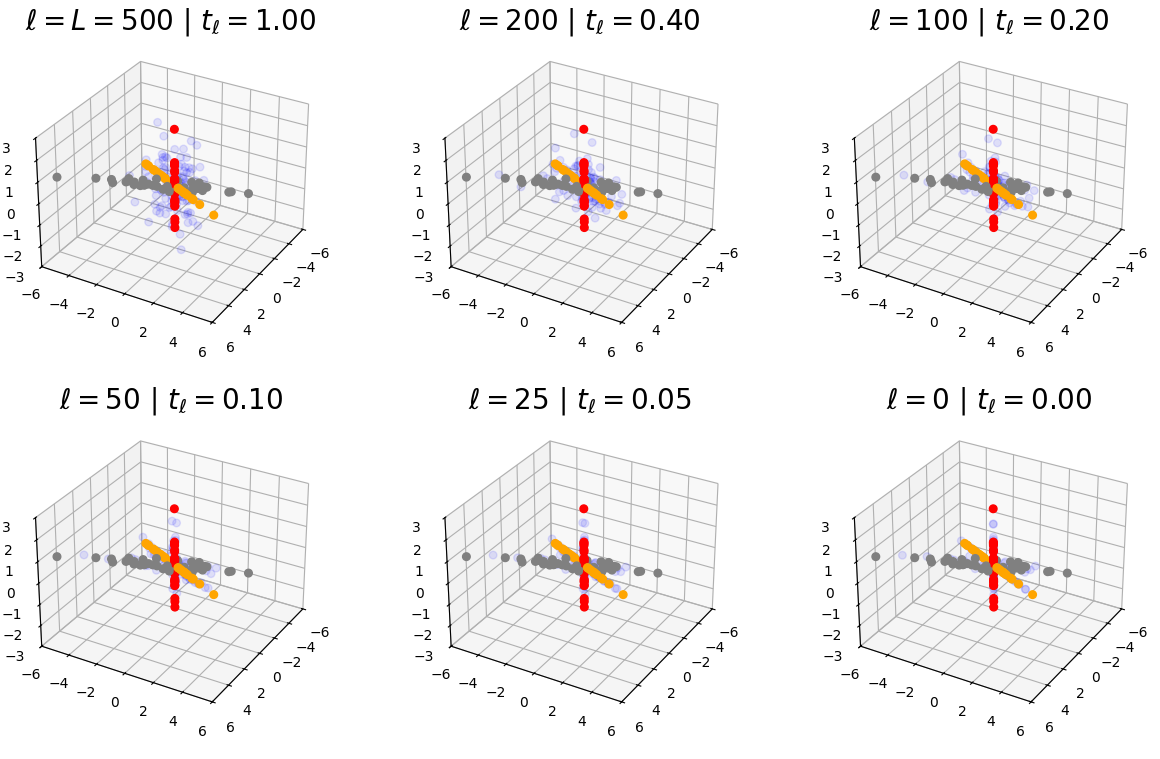
\includegraphics[width=\textwidth]{\toplevelprefix/chapters/chapter3/figs/vp_gmm_denoising.png}
	\caption{\small\textbf{使用 VP 扩散过程去噪高斯混合模型。} 我们使用与 \Cref{fig:ve_gmm_denoising} 相同的图形设置和数据分布。注意,与 \Cref{fig:ve_gmm_denoising} 相比,噪声分布更集中在原点附近。}
	\label{fig:vp_gmm_denoising}
\end{figure}

\begin{algorithm}
	\caption{使用去噪器进行采样。}
	\label{alg:iterative_denoising}
	\begin{algorithmic}[1]
		\Require{一个用于采样的有序时间步列表 \(0 \leq t_{0} < \cdots < t_{L} \leq T\)。}
		\Require{一个去噪器 \(\bar{\vx} \colon \{t_{\ell}\}_{\ell = 1}^{L} \times \R^{D} \to \R^{D}\)。}
		\Require{尺度和噪声水平函数 \(\alpha, \sigma \colon \{t_{\ell}\}_{\ell = 0}^{L} \to \R_{\geq 0}\)。}
		\Ensure{一个样本 \(\hat{\vx}\),近似来自 \(\vx\) 的分布。}
		\Function{DDIMSampler}{$\bar{\vx}, (t_{\ell})_{\ell = 0}^{L}$}
		\State{初始化 \(\tilde{\vx}_{t_{L}} \sim\) \(\vx_{t_{L}}\) 的近似分布} \Comment{VP \(\implies \dNorm(\vzero, \vI)\),VE \(\implies \dNorm(\vzero, t_{L}^{2}\vI)\)。}
		\For{\(\ell = L, L - 1, \dots, 1\)}
		\State{计算
			\begin{equation*}
				\hat{\vx}_{t_{\ell - 1}} \doteq \frac{\sigma_{t_{\ell - 1}}}{\sigma_{t_{\ell}}}\hat{\vx}_{t_{\ell}} + \bp{\alpha_{t_{\ell - 1}} - \frac{\sigma_{t_{\ell - 1}}}{\sigma_{t_{\ell}}}\alpha_{t_{\ell}}}\bar{\vx}(t_{\ell}, \hat{\vx}_{t_{\ell}})
			\end{equation*}
		}
		\EndFor
		\State{\Return{\(\hat{\vx}_{t_{0}}\)}}
		\EndFunction
	\end{algorithmic}
\end{algorithm}

\paragraph{步骤 3:优化训练流程。} 如果我们使用 \Cref{sub:intro_diffusion_denoising} 中规定的程序来为采样算法中要使用的每个时间 \(t\) 学习一个单独的去噪器 \(\bar{\vx}(t, \cdot)\),\textit{我们就必须学习 \(L\) 个单独的去噪器!} 这是非常低效的——通常情况下,我们必须训练 \(L\) 个独立的神经网络,占用 \(L\) 倍的训练时间和存储内存,然后永远被锁定在使用这些时间步进行采样。相反,我们可以\textit{训练一个单一的神经网络}来在所有时间 \(t\) 上进行去噪,将连续变量 \(\vx_{t}\) 和 \(t\) 作为输入(而不仅仅是之前的 \(\vx_{t}\))。在机制上,我们的训练损失在 \(t\) 上取平均,即解决以下问题:
\begin{equation}
	\min_{\theta}\Ex_{t, \vx, \vx_{t}}\norm{\bar{\vx}_{\theta}(t, \vx_{t}) - \vx}_{2}^{2}.
\end{equation}
与步骤 1 类似,我们使用更多靠近 \(t = 0\) 的时间步来确保更好的采样过程,我们可能希望确保去噪器在靠近 \(t = 0\) 时质量更高,因此\textit{对损失进行加权},使得靠近 \(0\) 的 \(t\) 具有更高的权重。设 \(w_{t}\) 是时间 \(t\) 的权重,加权损失将如下所示
\begin{equation}\label{eq:parametric_denoising_loss}
	\min_{\theta}\Ex_{t}w_{t}\Ex_{\vx, \vx_{t}}\norm{\bar{\vx}_{\theta}(t, \vx_{t}) - \vx}_{2}^{2}.
\end{equation}
在实践中,一个合理的权重选择是 \(w_{t} = \alpha_{t}/\sigma_{t}\)。确切的原因将在下一段中介绍,但总的来说,它用于增加对应于接近 \(0\) 的 \(t\) 的损失的权重,同时保持合理的数值稳定性。当然,在实践中我们无法计算期望,所以我们使用最直接的蒙特卡洛平均来估计它。这里所做的一系列更改有几个概念上和计算上的好处:我们不需要训练多个去噪器,我们可以在一组时间步上训练,并使用一个子集(或完全其他的)进行采样,等等。完整的流程在 \Cref{alg:learning_denoiser} 中讨论。

\begin{algorithm}
	\begin{algorithmic}[1]
		\Require{数据集 \(\cD \subseteq \R^{D}\)。}
		\Require{一个用于采样的有序时间步列表 \(0 \leq t_{0} < \cdots < t_{L} \leq T\)。}
		\Require{一个加权函数 \(w \colon \{t_{\ell}\}_{\ell = 1}^{L} \to \R_{\geq 0}\)。}
		\Require{尺度和噪声水平函数 \(\alpha, \sigma \colon \{t_{\ell}\}_{\ell = 0}^{L} \to \R_{\geq 0}\)。}
		\Require{一个参数空间 \(\Theta\) 和一个去噪器架构 \(\bar{\vx}_{\theta}\)。}
		\Require{一个用于参数的优化算法。}
		\Require{优化迭代次数 \(M\)。}
		\Require{每次迭代的蒙特卡洛抽样次数 \(N\)(用于近似 \eqref{eq:parametric_denoising_loss} 中的期望)}
		\Ensure{一个训练好的去噪器 \(\bar{\vx}_{\theta^{\ast}}\)。}

		\Function{TrainDenoiser}{$\cD, \Theta$}
		\State{初始化 \(\theta^{(1)} \in \Theta\)}
		\For{\(i \in [M]\)}
		\For{\(n \in [N]\)}
		\State{\(\vx_{n}^{(i)} \sim \cD\)} \Comment{从数据集中抽取一个样本。}
		\State{\(t_{n}^{(i)} \simiid \dUnif(\{t_{\ell}\}_{\ell = 1}^{L})\)} \Comment{采样一个时间步。}
		\State{\(\vg_{n}^{(i)} \simiid \dNorm(\vzero, \vI)\)} \Comment{采样一个噪声向量。}
		\State{\(\vx_{t, n}^{(i)} \doteq \alpha_{t_{n}^{(i)}}\vx_{n}^{(i)} + \sigma_{t_{n}^{(i)}}\vg_{n}^{(i)}\)} \Comment{计算加噪样本。}
		\State{\(w_{n}^{(i)} \doteq w_{t_{n}^{(i)}}\)} \Comment{计算损失权重。}
		\EndFor
		\State{\(\hat{\cL}^{(i)} \doteq \displaystyle \frac{1}{N}\sum_{n = 1}^{N}w_{n}^{(i)}\norm{\vx_{n}^{(i)} - \bar{\vx}_{\theta^{(i)}}(t_{n}^{(i)}, \vx_{t, n}^{(i)})}_{2}^{2}\)} \Comment{计算损失估计。}
		\State{\(\theta^{(i + 1)} \doteq \texttt{OptimizationUpdate}^{(i)}(\theta^{(i)}, \nabla_{\theta^{(i)}}\hat{\cL}^{(i)})\)} \Comment{更新参数。}
		\EndFor
		\State{\Return{\(\bar{\vx}_{\theta^{(K + 1)}}\)}}
		\EndFunction
	\end{algorithmic}
	\caption{从数据中学习去噪器。}
	\label{alg:learning_denoiser}
\end{algorithm}

\paragraph{(可选)步骤 4:改变估计目标。} 注意,通常的做法是将整个去噪流程重新定位到\textit{噪声预测器}上,即对 \(\Ex[\vg \mid \vx_{t}]\) 的估计。在实践中,噪声预测器稍微更容易训练,因为它们的输出(几乎)总是与高斯随机变量的大小相当,所以训练在数值上更稳定。注意,根据 \eqref{eq:gen_additive_gaussian_noise_model} 我们有
\begin{equation}
	\vx_{t} = \alpha_{t}\Ex[\vx \mid \vx_{t}] + \sigma_{t}\Ex[\vg \mid \vx_{t}] \implies \Ex[\vg \mid \vx_{t}] = \frac{1}{\sigma_{t}}\bp{\vx_{t} - \alpha_{t}\Ex[\vx \mid \vx_{t}]},
\end{equation}
因此,任何对 \(\vx\) 的预测器都可以使用上述关系转化为对 \(\vg\) 的预测器,即
\begin{equation}
	\bar{\vg}(t, \vx_{t}) = \frac{1}{\sigma_{t}}\vx_{t} - \frac{\alpha_{t}}{\sigma_{t}}\bar{\vx}(t, \vx_{t}),
\end{equation}
反之亦然。因此,一个好的估计 \(\bar{\vg}\) 的网络与一个好的估计 \(\bar{\vx}\) 的网络相同,\textit{外加一个残差连接}(如在 Transformer 中所见)。它们的损失也与去噪器相同,只是多了一个因子 \(\alpha_{t}/\sigma_{t}\),即
\begin{equation}
	\Ex_{t}w_{t}\Ex_{\vg, \vx_{t}}\norm{\vg - \bar{\vg}(t, \vx_{t})}_{2}^{2} = \Ex_{t}w_{t}\frac{\alpha_{t}^{2}}{\sigma_{t}^{2}}\Ex_{\vx, \vx_{t}}\norm{\vx - \bar{\vx}(t, \vx_{t})}_{2}^{2}.
\end{equation}
为了完整起见,我们将提到其他目标也已被提出用于不同的任务,例如 \(\Ex[\odv*{\vx_{t}}{t} \mid \vx_{t}]\)(称为 \(v\)-预测或速度预测)等,但去噪和噪声预测仍然是常用的。在本书的其余部分,我们将只考虑去噪。


我们对我们最初的柏拉图式的加噪/去噪过程做了很多改变。为了确保新过程在实践中仍然有效,我们可以计算数值例子(例如 \Cref{fig:vp_gmm_denoising})。为了确保它在理论上是健全的,我们可以为采样算法证明一个\textit{误差率界限},这表明采样器的输出分布在所谓的\textit{全变分(TV)距离}上收敛到真实分布。TV 距离定义在两个随机变量 \(\vx\) 和 \(\vy\) 之间为:
\begin{equation}
	\TV(\vx, \vy) \doteq \sup_{A \subseteq \R^{d}}\abs*{\Pr[\vx \in A] - \Pr[\vy \in A]}.
\end{equation}
如果 \(\vx\) 和 \(\vy\) 非常接近(一致地),那么上确界将很小。所以 TV 距离衡量随机变量的接近程度。(它确实是一个度量,正如其名所示:证明是一个练习。)

\begin{theorem}[\citep{li2024d} 定理 1,简化版]\label{thm:diffusion_sampler_convergence}
	假设 \(\Ex\norm{\vx}_{2} < \infty\)。如果 \(\vx\) 根据 VP 过程使用指数离散化\footnote{精确的定义在我们的符号体系中相当冗长,并且只定义到各种绝对常数,所以为了简洁起见我们在此省略。当然它在原始论文 \citep{li2024d} 中。}(如 \eqref{eq:denoising_exponential_discretization} 中)进行去噪,\Cref{alg:iterative_denoising} 的输出 \(\hat{\vx}\) 满足全变分界
	\begin{equation}\label{eq:diffusion_sampling_error}
		\TV(\vx, \hat{\vx}) = \tilde{\cO}\rp{\underbrace{\frac{D}{L}}_{\text{离散化误差}} + \underbrace{\sqrt{\frac{1}{L}\sum_{\ell = 1}^{L}\frac{\alpha_{t_{\ell}}}{\sigma_{t_{\ell}}^{2}}\Ex_{\vx, \vx_{t_{\ell}}}\norm{\bar{\vx}^{\ast}(t_{\ell}, \vx_{t_{\ell}}) - \bar{\vx}(t_{\ell}, \vx_{t_{\ell}})}_{2}^{2}}}_{\text{去噪器的平均超额误差}}}
	\end{equation}
	其中 \(\bar{\vx}^{\ast}\) 是 \(\vx\) 的贝叶斯最优去噪器,\(\tilde{\cO}\) 是忽略 \(L\) 中对数因子的大-\(\cO\) 符号的一个版本。
\end{theorem}
非常高层次的证明技巧是,如前所述,在每一步都对误差进行界定,区分误差来源(离散化和去噪器误差),并仔细确保误差不会累积过多(甚至相互抵消)。

注意,如果 \(L \to \infty\) 并且我们正确地学习了贝叶斯最优去噪器 \(\bar{\vx} = \bar{\vx}^{\ast}\)(使得超额误差为 \(0\)),那么 \Cref{alg:iterative_denoising} 中的采样过程将产生一个加噪过程的\textit{完美(在分布上)逆过程},因为 \Cref{thm:diffusion_sampler_convergence} 中的误差率趋于 \(0\),\footnote{对于 VE 过程也有类似的结果,尽管据我们所知没有一个像这个一样清晰。} 正如之前启发式地论证的那样。

\begin{remark}
	如果数据是低维的,比如说,支持在高维空间 \(\R^{D}\) 的一个\textit{低秩子空间}上怎么办?如果数据分布是紧支撑的——比如说,如果数据被归一化到单位超立方体,这通常作为真实数据(如图像)的预处理步骤来确保——那么有可能做得更好。也就是说,\cite{li2024d} 的作者还使用所谓覆盖数的渐近性定义了一种\textit{近似内在维度}的度量,这在直觉上(如果不是在实现上)与下一节中介绍的率失真函数非常相似。然后他们表明,使用 \Cref{alg:iterative_denoising} 中 DDIM 采样器的一个特定的小修改(即,稍微扰动更新系数),离散化误差变为
	\begin{equation}
		\tilde{\cO}\rp{\frac{\text{近似内在维度}}{L}}
	\end{equation}
	而不是像 \Cref{thm:diffusion_sampler_convergence} 中的 \(\frac{D}{L}\)。因此,使用这种修改后的算法,即使 \(D\) 达到数千或数百万,\(L\) 也不必太大,因为真实数据具有低维结构。然而,在实践中我们使用 DDIM 采样器,所以 \(L\) 应该对 \(D\) 有一个温和的依赖性,以实现一致的误差率。\(L\) 的确切选择是在采样的计算复杂性(例如,运行时间或内存消耗)和学习低维结构的去噪器的统计复杂性之间进行权衡。\(L\) 的值在训练时(其中较大的 \(L\) 允许更好地覆盖区间 \([0, T]\),这有助于网络学习一个在 \(t\) 上泛化的关系)和采样时(其中较小的 \(L\) 意味着更高效的采样)通常是不同的。人们甚至可以在采样时自适应地选择时间步,以优化这种权衡 \cite{bao2022analytic}。
\end{remark}

\begin{remark}
	其他各种工作将逆过程定义为使用显式差分方程或在极限 \(L \to \infty\) 时的微分方程在时间索引 \(t\) 上向后移动,或者使用变换 \(\vy_{t} = \vx_{T - t}\) 在时间上向前移动,这样如果 \(t\) 增加,\(\vy_{t}\) 就变得更接近 \(\vx_{0}\)。在这项工作中,我们努力保持一致性:我们随时间向前进行加噪,随时间向后进行去噪。如果你正在阅读另一篇在时间索引上不清楚的著作,或者试图实现一个同样不清楚的算法,有一种方法可以每次都做对:采样过程在从一步移动到下一步时,去噪器项和当前迭代项的系数都应该总是\textit{正的}。但总的来说,许多论文定义了自己的符号,对用户不友好。
\end{remark}

\begin{remark}
	上一节 \Cref{sub:intro_diffusion_denoising} 末尾提出的理论似乎(粗略地说)表明,在实践中,使用类 Transformer 网络是学习或近似去噪器的一个好选择。这是合理的,但是使用任何旧的神经网络(例如多层感知器(MLP))并试图将其无限扩展有什么问题呢?为了观察这个问题,让我们看一个在 \Cref{example:denoising_gaussian_mixture} 中研究的高斯混合模型的另一个特例。即,\textit{经验分布}是一个退化高斯混合模型的实例,有 \(K = N\) 个成分 \(\dNorm(\vx_{i}, \vzero)\),以相等的概率 \(\pi_{i} = \frac{1}{N}\) 采样。在这种情况下,贝叶斯最优去噪器是
	\begin{equation}\label{eq:memorizing_denoiser}
		\bar{\vx}^{\star}(t, \vx_{t}) = \sum_{i = 1}^{N}\frac{e^{-\|\vx_{t} - \alpha_{t}\vx_{i}\|_{2}^{2}/(2\sigma_{t}^{2})}}{\sum_{j = 1}^{N}e^{-\|\vx_{t} - \alpha_{t}\vx_{j}\|_{2}^{2}/(2\sigma_{t}^{2})}}\vx_{i}.
	\end{equation}
	这是数据 \(\vx_{i}\) 的一个凸组合,并且当 \(t \to 0\) 时,系数变得“更尖锐”(即,更接近 \(0\) 或 \(1\))。请注意,当我们根据从固定有限数据集 \(\vX = \{\vx_{i}\}_{i = 1}^{N}\) 中均匀随机抽取 \(\vx\) 来计算损失时,这个去噪器\textit{最优地解决了}去噪优化问题 \eqref{eq:parametric_denoising_loss},这是一个非常现实的设置。因此,如果我们的网络架构 \(\bar{\vx}_{\theta}\) 足够富有表现力,以至于可以很好地近似上述形式 \eqref{eq:memorizing_denoiser} 的最优去噪器,那么学习到的去噪器可能就会这样做。然后,我们的迭代去噪 \Cref{alg:iterative_denoising} 将精确地从经验分布中采样,重新生成训练数据中的样本,正如 \Cref{thm:diffusion_sampler_convergence} 所证明的那样。这是一个糟糕的采样器,并不比一个包含所有样本的数据库更有趣,因此理解如何在实践中避免这种情况非常重要。关键是提出一种能够很好地近似真实去噪器(例如对应于 \eqref{eq:gmm_lowrank_denoiser} 中的低秩分布)但不能很好地近似如 \eqref{eq:memorizing_denoiser} 中的经验贝叶斯去噪器的网络架构。一些工作已经探讨了这条细微的界线,以及为什么使用基于 Transformer 和卷积的网络架构的现代扩散模型可以在不同机制下记忆和泛化 \citep{kamb2024analytic,niedoba2024towards}。

	在较高的层次上,一个记忆所有训练点的去噪器,如 \eqref{eq:memorizing_denoiser} 中所示,对应于一个具有最小编码率的分布的参数模型,并通过单独编码每个样本来实现这一点。我们将在下一节从信息论的角度讨论这个问题(以及与我们在 \Cref{sub:min_entropy} 末尾提出的初始期望的表面矛盾)。
\end{remark}

\section{通过有损编码进行压缩} \label{sec:lossy_compression}

让我们回顾一下到目前为止我们已经涵盖的内容。我们已经讨论了如何使用有限样本拟合一个\textit{去噪器} \(\bar{\vx}_{\theta}\)。我们展示了这个去噪器编码了一个分布,因为它通过特威迪公式 \eqref{eq:tweedie} 与其对数密度直接相关。然后,我们用它通过\textit{迭代去噪}将一个纯噪声(高熵)分布逐渐转变为学习到的分布。因此,我们已经发展了在 \Cref{sub:min_entropy} 末尾提出的第一种学习或追求分布的方式。

然而,在这种方法论中,分布的编码隐含在去噪器的函数形式和参数中(如果有的话)。事实上,敏锐的读者可能已经注意到,对于一个一般的分布,我们从未明确指定去噪器的函数形式是什么。在实践中,人们通常用一些具有经验设计的架构的深度神经网络来建模它。此外,虽然我们知道上述去噪过程降低了熵,但我们不知道降低了多少,也不知道中间和最终分布的熵。

回想一下,我们的总体目标是为来自具有低维支撑的(连续)分布的数据建模。如果我们的目标是识别生成数据的“最简单”模型,可以考虑三种典型的简约性度量:维度、体积或(微分)熵。那么,如果使用维度,那么对于给定的数据集,最好的模型显然是经验分布本身,它是零维的。对于所有具有低维支撑的分布,微分熵总是负无穷大;它们的支撑集的体积总是零。那么,在所有可能生成相同数据样本的低维支撑的分布中,我们如何根据这些根本无法区分低维模型的简约性度量来决定哪一个更好呢?本节旨在解决这个看似令人困惑的情况。

在本章的其余部分,我们讨论一个框架,该框架允许我们通过将学习到的分布与一个明确的可计算的编码和解码方案相关联来缓解上述技术困难,遵循在 \Cref{sub:min_entropy} 末尾建议的第二种方法。正如我们将看到的,这种方法基本上允许我们根据与编码方案相关的(有损)编码长度或编码率来准确地近似学习到的分布的熵。有了这样的度量,我们不仅可以准确地测量任何处理(包括去噪)分布所减少的熵,从而获得的信息,而且我们还可以推导出能够以最有效的方式进行此类操作的最优算子的明确形式。正如我们将在下一章 \Cref{ch:representation} 中看到的,这将导致对深度网络架构的原则性解释,以及更高效的深度架构设计。

\subsection{有损编码的必要性}

%\yima{I need to completely rewrite the  transition below as motivation for rate distortion... }

%\yima{Lossy coding does more than just quantization. It allows us to avoid pathological solution by simply using the empirical distribution as the optimal solution that minimizes entropy. How to elaborate this point?}

我们之前多次讨论过一个困难:如果我们最终从有限的样本中学习分布,并且我们的去噪器函数类包含足够多的函数,我们如何确保我们从\textit{真实的}分布(具有低维支撑)中采样,而不是从任何其他可能以高概率产生这些有限样本的分布中采样?让我们通过一些具体的例子来揭示一些概念上和技术上的困难。

\begin{example}[体积、维度和熵]\label{eg:measures-of-complexity}
对于图 \ref{fig:1d-line} 顶部所示的例子,假设我们从一条线上的均匀分布(比如在二维平面上)中抽取了一些样本。这条线或样本集的体积为零。
从几何上看,在产生的有限样本集上的经验分布是能够产生该有限样本集的{\em 最小维度}的分布。\footnote{一组离散样本都是零维的,而支撑线是一维的。} 但这与另一个复杂性度量——熵——似乎形成了对比。这条线的(微分)熵是负无穷大,但这个样本集的(离散)熵是有限且为正的。因此,根据这些常见的简约性或复杂性度量,我们似乎处于一个矛盾的境地:它们根本无法正确地区分(用于)低维支撑分布的(模型),有些甚至似乎以完全相反的方式区分它们。\footnote{当然,严格来说,微分熵和离散熵是不能直接比较的。}
\end{example}

\begin{example}[密度]\label{eg:density} 考虑图 \ref{fig:1d-line} 中所示的两组采样数据点。从几何上看,它们本质上是相同的:每组包含八个点,每个点以相等的频率 $1/8$ 出现。唯一的区别是,对于第二组数据,一些点“足够近”,可以被视为在其各自的“聚类”周围具有更高的密度。哪一个与可能生成样本的真实分布更相关?我们如何调和解释这种(经验)分布时的模糊性?
\begin{figure}[t]
	\centering
	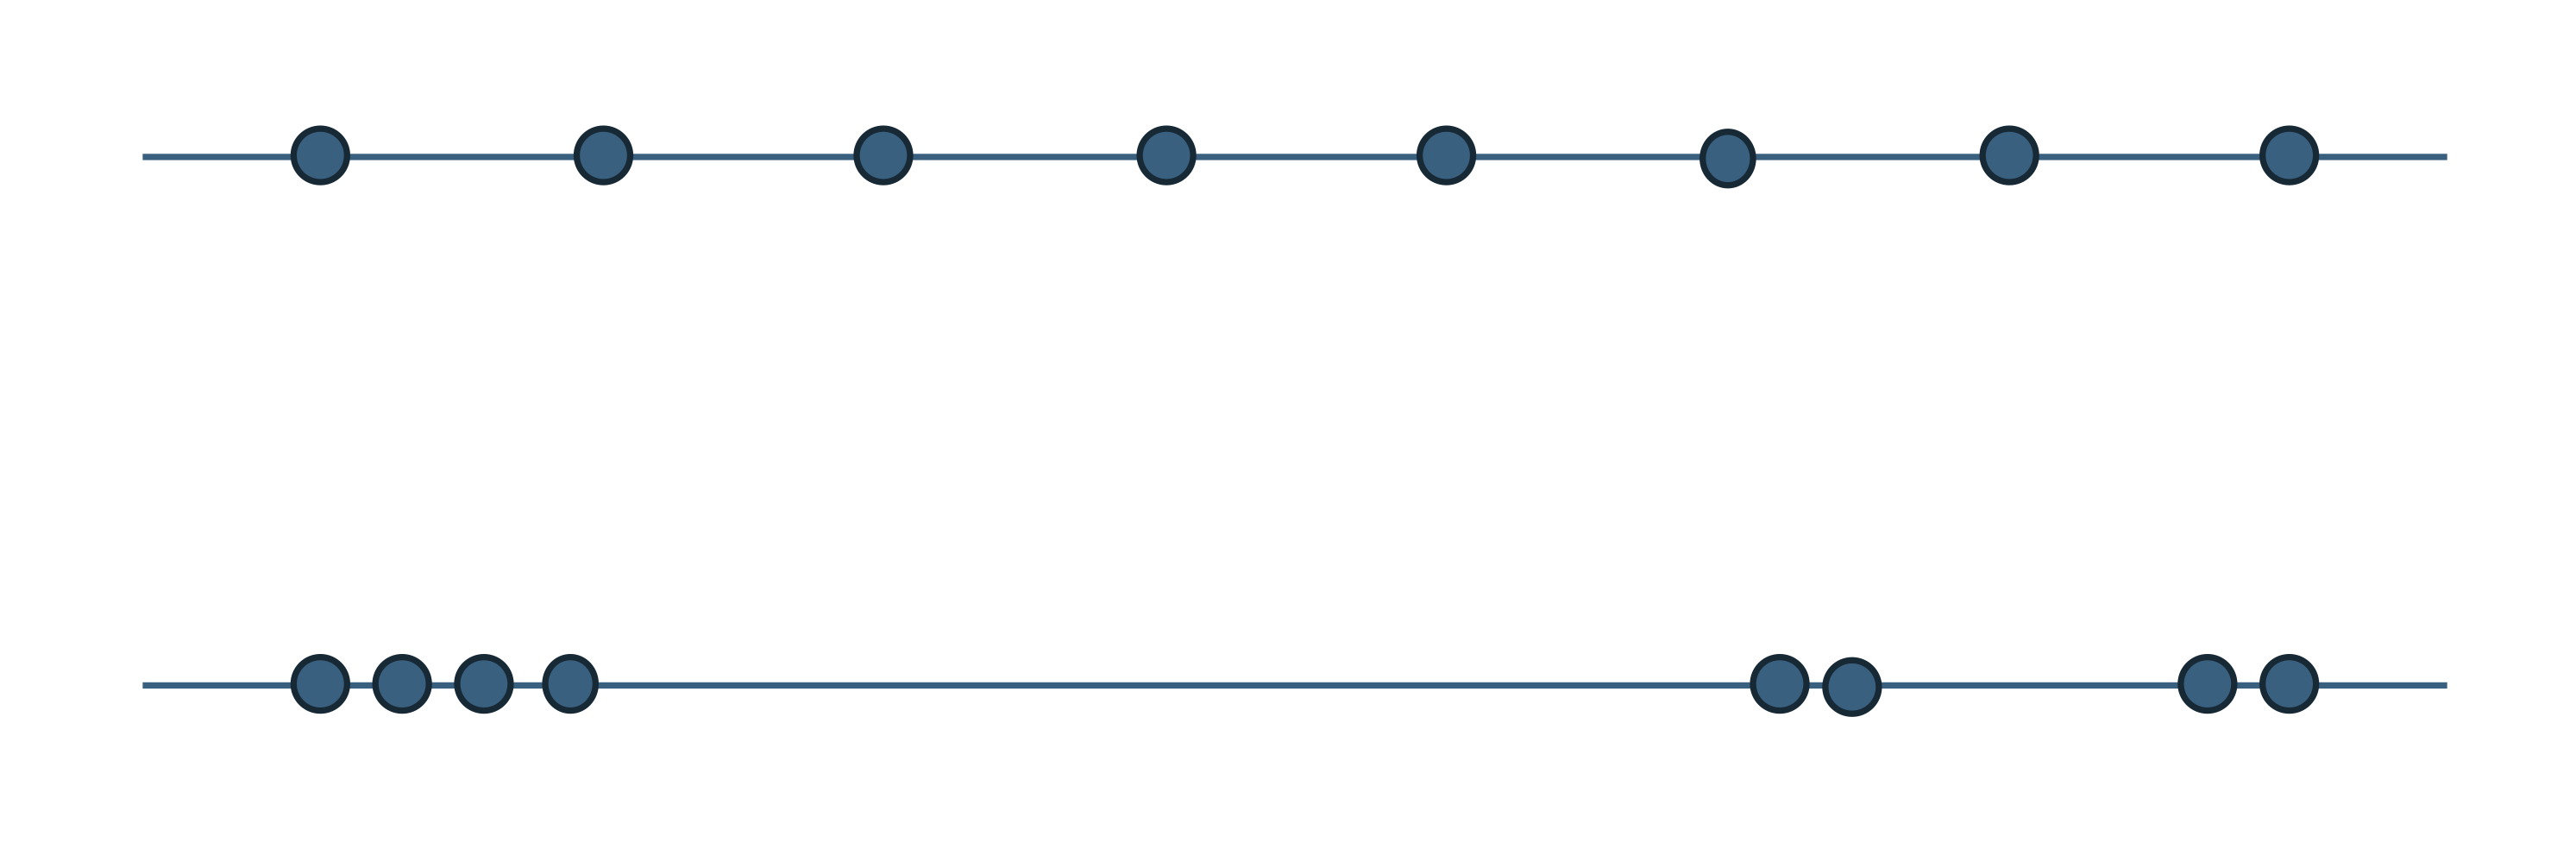
\includegraphics[width=0.7\linewidth]{\toplevelprefix/chapters/chapter3/figs/one-dim-distribution.png}
	\caption{在一条线上观察到的八个点。}
	\label{fig:1d-line}
\end{figure}
\end{example}


% If the (geometric) volume is not a suitable measure of parsimony or compression for a (finite-sampled empirical) distribution, then maybe the {entropy}, or {\em the minimum coding rate}, associated with true probability (density or distribution) of those samples $p(\vx_i)$ is a better measure. Although many results like Theorem \ref{thm:distribution-convergence} \yima{missing reference...} ensure convergence to the true distribution (hence entropy) in the asymptotic regime\footnote{That is, when the sample size goes to infinity.}, it is not so clear when and how one can simultaneously infer the distribution and conduct the compression correctly in the {\em non-asymptotic} regime when we are given only a fixed set of samples, as the cases shown in Figure \ref{fig:1d-line}. It is observed empirically that sampling Algorithm \ref{alg:iterative_denoising} (with diffusion/denoising models) tends to generalize beyond just generating samples from the training set.

% Furthermore, besides the entropy of the data distribution, there are in fact other fundamental constraints and costs associated with implementing an encoding-decoding scheme for any given data set. This section attempts to address some of these issues from a constructive perspective regarding learning and representing a data distribution from a finite set of samples.


%\yima{From computable (entropy) to implementable. That is, in addition to a computable or achievable encoding scheme, there should also exist an implementable decoding scheme. Lossy quantization becomes necessary for real-valued data.}

在为数据集构建显式编码和解码方案时,还存在另一个技术难题。给定一个采样数据集 $\X = [\vx_1, \ldots, \vx_N]$,如何设计一个可以在有限内存和计算资源的机器上实现的编码方案?请注意,即使表示一个普通的实数也需要无限数量的数字或比特。因此,人们可能会想,一个分布的熵是否是其(最优)编码方案复杂性的直接度量。我们用另一个简单的例子来研究这个问题。
\begin{example}[精度] \label{eg:two-inrational}
	考虑一个离散分布 $\X = [e, \pi]$,它以相等的概率 $1/2$ 取欧拉数 $e \approx 2.71828$ 或圆周率 $\pi \approx 3.14159$ 的值。这个分布的熵是 $H =1$,这表明可以用一个一位的二进制数字 $0$ 或 $1$ 来分别编码这两个数。但是你能在有限状态机上实现这个编码的解码方案吗?答案其实是否定的,因为精确描述这两个数中的任何一个都需要无限多的比特。
\end{example}

因此,通常不可能有一个能够精确再现来自任意实值分布的样本的编码和解码方案。\footnote{也就是说,如果想要精确编码这样的样本,唯一的方法是记住每一个样本。} 但是,如果一个编码方案无法解码出同一分布的样本,那么它几乎没有实际价值。

因此,为了确保任何编码/解码方案都是可计算的,并且可以用有限的内存和计算资源实现,我们需要对样本 $\x$ 进行量化,并且只编码到一定的精度,比如 $\epsilon > 0$。{\em 这样做,本质上,我们认为任何两个距离小于 $\epsilon$ 的数据点是等价的。} 更准确地说,我们希望考虑编码方案
\begin{equation}
	\x \mapsto \hat \x
\end{equation}
使得由量化引起的期望误差以 $\epsilon$ 为界。从数学上讲更方便,概念上也几乎相同的是,将期望\textit{平方}误差以 \(\epsilon^{2}\) 为界,即
\begin{equation}
	\Ex[d(\vx, \hat \vx)^{2}] \le \epsilon^{2}.
\end{equation}
通常,距离 \(d\) 被选为欧几里得距离,或 2-范数。\footnote{更一般地,我们可以用任何所谓的\textit{散度}来代替 \(d^{2}\)。} 我们将在下文中采用这个选择。

\subsection{率失真与数据几何}
当然,在所有满足上述约束的编码方案中,我们希望选择能使最终编码率最小化的那一个。对于给定的随机变量 $\x$ 和精度 $\epsilon$,这个率被称为{\em 率失真},记作 $\cR_{\epsilon}(\x)$。
信息论中的一个深刻定理,最初由 \textcite{shannon1959coding} 证明,确立了这个率可以等价地用纯概率术语表示为
\begin{equation}
	% \cR_{\epsilon}(\x) = \min_{p(\hat \x \mid \x): \Ex[\norm{\x -\hat \x}_2^{2}] \le \epsilon^{2}} [h(\x) - h(\x \mid \hat{\x})],
	\cR_{\epsilon}(\x) 
	= \min_{p(\hat \x \mid \x): \Ex[\norm{\x -\hat \x}_2^{2}] \le \epsilon^{2}} 
	I(\vx; \hat{\vx}),
    \label{eqn:rate-distortion-general}
\end{equation}
其中量 $I(\vx; \hat{\vx})$ 被称为\textit{互信息},定义为
\begin{equation}\label{eq:mutual-information}
	I(\vx; \hat{\vx})
	= \KL(p(\vx, \hat{\vx}) \mmid p(\vx) p(\hat{\vx})).
\end{equation}
注意,\eqref{eqn:rate-distortion-general} 中的最小化是在所有满足失真约束 $\Ex_{\x, \hat \x}[\norm{\x- \hat \x}_2^{2}] \le \epsilon^{2}$ 的条件分布 $p(\hat \x \mid \x)$ 上进行的。每个这样的条件分布都导出一个联合分布 $p(\vx,
\hat{\vx}) = p(\hat\x \mid \x) p(\x)$,它决定了互信息 \eqref{eq:mutual-information}。互信息的许多方便性质(以及因此的率失真)都由 KL 散度的相应性质所暗示(回顾 \Cref{thm:information-inequality})。根据定义,我们知道 $\cR_{\epsilon}(\x)$ 是一个关于 $\epsilon$ 的{\em 非增}函数。

\begin{remark}
	事实证明,率失真在以下意义上是 \(\x\) 的熵的一个可实现的近似。
	假设 \(\vx\) 和 \(\hat{\vx}\) 是连续随机向量。
	那么互信息可以写成
	\begin{equation}\label{eq:information-entropy}
		I(\x; \hat\x) = h(\x) - h(\x \mid \hat \x),
	\end{equation}
	其中 $h(\x \mid \hat \x) = \bE[\log_2 p(\x \mid \hat\x)]$ 是给定 \(\hat \x\) 时 \(\x\) 的\textit{条件熵}。
	% Notice that in Information Theory, the quantity $h(\x) - h(\x \mid \hat \x)$
	% is known as {\em the mutual information} $I(\x; \hat \x)$ between the two
	% variables $\x$ and $\hat \x$. See \cite{Cover-Thomas} for more details.
	因此,最小编码率是在所有满足约束 $\mathbb{E} [\norm{\x- \hat \x}_2^2] \le \epsilon^2$ 的分布中,当 \(\x\) 的熵与给定 \(\hat \x\) 时 \(\x\) 的条件熵之间的差值最小时实现的。
	% From
	% the properties of mutual information $I(\x; \hat \x) = I(\hat \x; \x)$, we
	% have\footnote{The subsequent assertion assumes for simplicity that the reconstruction
	% $\hat{\vx}$ is also a continuous random vector, so that the differential
	% entropy is well-defined. More generally, advanced
	% mathematical notions from measure theory can be used to define the mutual
	% information irrespective of whether or not $\vx$ and $\hat{\vx}$ are
	% continuous or discrete: see \textcite[\S 8.5]{Cover-Thomas}.}
	% \begin{equation}
 %        h(\x) - h(\x \mid \hat{\x}) = h(\hat\x) - h(\hat\x \mid {\x}).
 %    \end{equation}
 %    Hence, the above rate distortion \eqref{eqn:rate-distortion-general} can also be rewritten as:
 %    \begin{equation}
	% 	\cR_{\epsilon}(\x) = \min_{p(\hat \vx \mid \vx): \mathbb{E} [\norm{\x-
	% 	\hat \x}_2^{2}] \le \epsilon^{2}} [H(\hat \x) - H(\hat \x \mid \x)].  \label{eqn:rate-distortion-general-2}
	% \end{equation}

	事实上,要得出上述类型的结论,并不需要假设 \(\x\) 和 \(\hat \x\) 是连续的。例如,如果两个随机向量都是离散的,那么在对离散值随机向量的 KL 散度进行适当解释后,我们有
	\begin{equation}
		I(\x; \hat\x) = H(\x) - H(\x \mid \hat \x).
	\end{equation}
	更一般地,可以使用测度论中的高级数学概念来定义任意随机变量 \(\x\) 和 \(\hat \x\) 的互信息(以及因此的率失真),包括那些具有相当奇异的低维分布的变量;参见 \textcite[\S 8.5]{Cover-Thomas}。
\end{remark}

\begin{remark}
    给定一组数据点 $\X = [\x_1,\ldots, \x_N]$,人们总是可以将其解释为来自一个均匀离散分布的样本,该分布在这些 $N$ 个向量上具有相等的概率 $1/N$。这样一个分布的熵是 $H(\X) = \frac{1}{N}\log_2 N$。\footnote{再次注意,即使我们可以用这个编码率来编码这些向量,我们也无法以任意精度解码它们。} 然而,即使 $\X$ 是其样本上的一个均匀分布,如果这些样本分布不那么均匀,并且许多样本聚集在一起,那么用有损编码方案可实现的编码率 $\cR_{\epsilon}(\X)$ 可能会显著低于 $H(\X)$。因此,对于图 \ref{fig:1d-line} 中显示的第二种分布,对于一个适当选择的量化误差 $\epsilon$,可实现的有损编码率可以显著低于将其编码为均匀分布的编码率。\footnote{然而,对于这个离散均匀分布,当 $\epsilon$ 足够小时,我们总是有 $H(\X) \approx \cR_{\epsilon}(\X)$。} 还要注意的是,有了率失真的概念,在示例 \ref{eg:two-inrational} 中讨论的困难也消失了:我们可以选择两个足够接近这两个无理数的有理数。由此产生的编码方案将具有有限的复杂性。
\end{remark}

\begin{example}\label{example:sphere-covering-rate-distortion}
	有时,我们可能会面临相反的情况,即我们想先固定编码率,然后尝试找到一个能最小化失真的编码方案。例如,假设我们只想对从一个分布中采样的点使用固定数量的码字,我们想知道如何设计这些码字,使得在编码/解码方案中平均或最大失真最小化。例如,给定一个单位正方形上的均匀分布,我们想知道用比如说 $n$ 位能多精确地编码从这个分布中抽取的点。这个问题等价于问,我们可以用 $2^n$ 个半径为多少的圆盘覆盖这个单位正方形,使得半径(即失真)最小。图 \ref{fig:seven-circles-packing} 显示了用 \(n = 4, 6, 8\)(即分别为 \(2^{n} = 16, 64, 256\) 个圆盘)覆盖一个正方形的近似最优解。请注意,随着圆盘数量 \(2^{n}\) 的增加,圆盘的最优半径减小。
	\begin{figure}
		\centering
		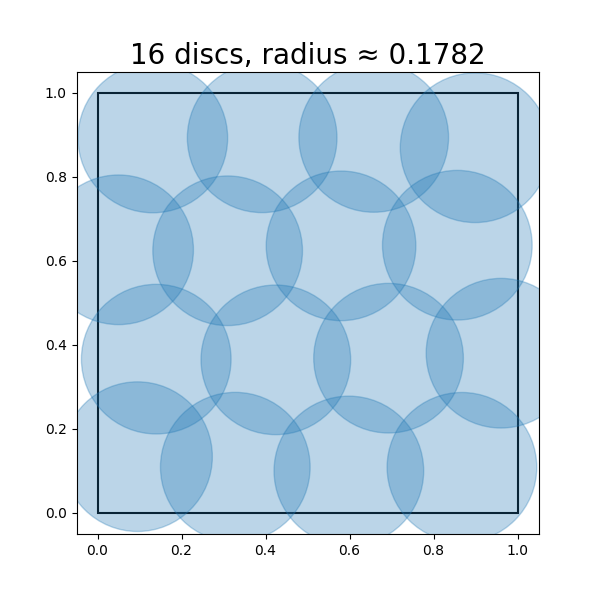
\includegraphics[width=0.3\textwidth]{\toplevelprefix/chapters/chapter3/figs/16.png}
		\hfill
		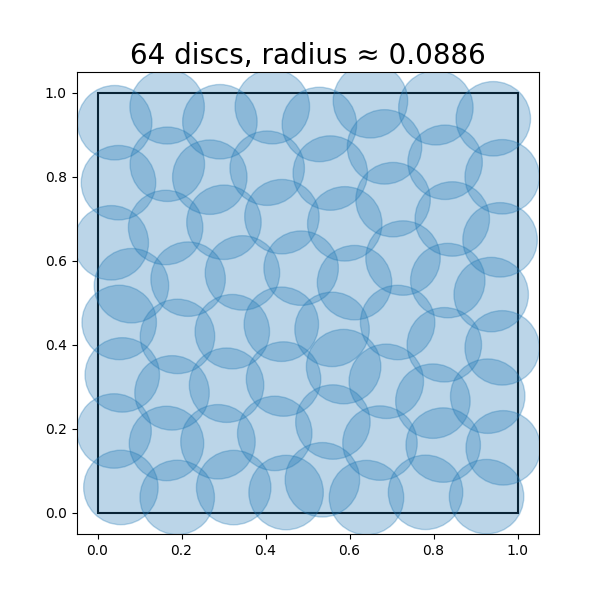
\includegraphics[width=0.3\textwidth]{\toplevelprefix/chapters/chapter3/figs/64.png}
		\hfill
		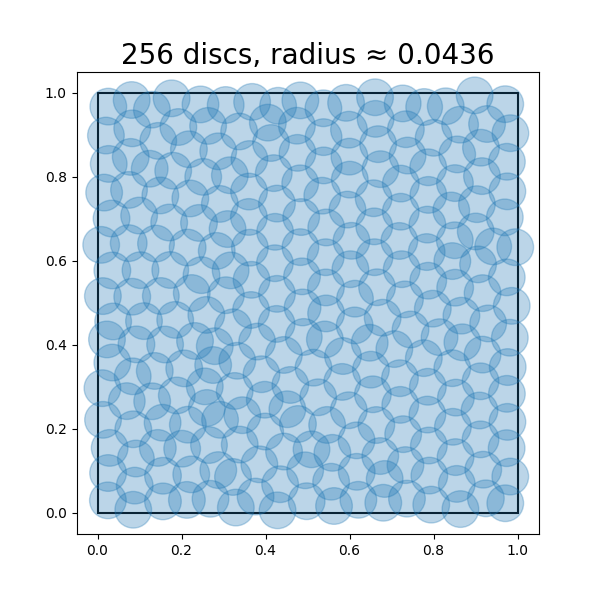
\includegraphics[width=0.3\textwidth]{\toplevelprefix/chapters/chapter3/figs/256.png}

		\caption{用 \(2^{4}\)、\(2^{6}\) 和 \(2^{8}\) 个圆盘覆盖一个正方形的最优解的近似,以及相应的半径,使用启发式优化算法计算得出。}
		\label{fig:seven-circles-packing}
	\end{figure}
\end{example}

\begin{figure}[t]
	\centering 
	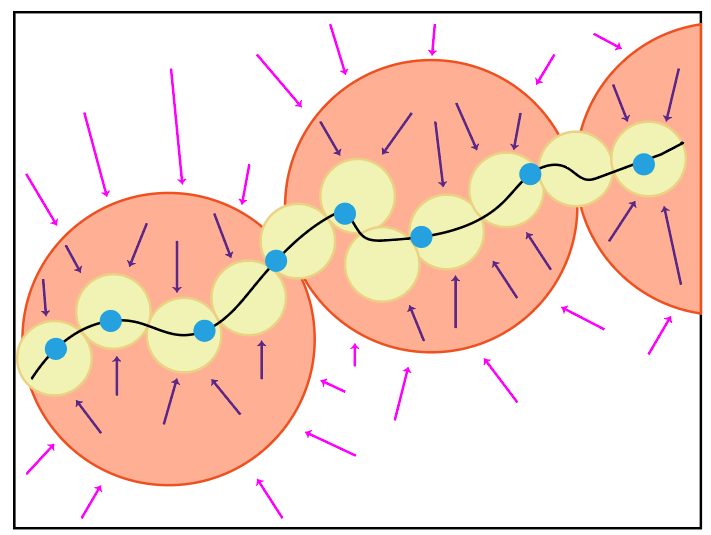
\includegraphics[width=0.6\textwidth]{\toplevelprefix/chapters/chapter3/figs/continuation.png}
	\caption{\small\textbf{用 \(\epsilon\) 球逼近低维分布。} 我们可以看到,随着 \(\epsilon\) 参数的缩小,\(\epsilon\)-球的并集越来越好地逼近真实分布(黑色)的支撑集。此外,通过将真实分布逼近为高斯混合模型(每个高斯分布的协方差为 \((\epsilon^{2}/D)\vI\))而获得的相关去噪器(其输入-输出映射由所提供的箭头给出)也越来越好地逼近真实的去噪器。在大的 \(\epsilon\) 下,这样的去噪器根本不指向真实分布附近,而在小的 \(\epsilon\) 下,它们紧密地逼近真实的去噪器。\Cref{thm:covering-number-rate-distortion} 确立了这种逼近在小失真 \(\epsilon\) 下刻画了率失真函数,统一了编码率最小化和去噪这两种并行的方法,用于学习没有病态的低维分布。}
	\label{fig:continuation}
\end{figure}

事实证明,对于一般的分布 $p(\vx)$,获得率失真函数 \eqref{eqn:rate-distortion-general} 的封闭形式表达式是一个非常困难的问题。然而,正如 \Cref{example:sphere-covering-rate-distortion} 所暗示的,在一些重要的特殊情况下,分布 $p(\vx)$ 的支撑集的\textit{几何}性质可以与率失真函数联系起来,从而与失真水平 $\epsilon$ 下的最优编码率联系起来。事实上,这个例子可以推广到任何 $p(\x)$ 的支撑集是一个足够规则的紧集的情况——包括低维分布——并且 $p(\x)$ 在其支撑集上是均匀分布的。这涵盖了大量具有实际意义的情况。我们在下面的结果中形式化了这个概念,它为一种特殊情况确立了这个性质。


% \DP{BEGIN SUS STUFF}
%
% The above example can be generalized to show that the rate distortion of a random variable \(\vx\) is very closely related to the so-called \textit{covering number} of the support of \(\vx\), given that this support is a compact set (e.g., bounded). Indeed, the covering number is exactly the number of balls with a finite radius that can cover the support of \(\vx\). We formalize this notion in the following proposition, to be proved in \Cref{exer:prop cover}.

\begin{theorem}\label{thm:covering-number-rate-distortion}
	假设 \(\vx\) 是一个随机变量,其支撑集 \(K \doteq \Supp(\vx)\) 是一个紧集。定义\textit{覆盖数} \(\cN_{\epsilon}(K)\) 为能够覆盖 \(K\) 的半径为 \(\epsilon\) 的球的最小数量,即
	\begin{equation}
		\cN_{\epsilon}(K) \doteq \min\left\{n \in \bN \colon \exists \vp_{1}, \dots, \vp_{n} \in K\ \text{s.t.}\ K \subseteq \bigcup_{i = 1}^{n}B_{\epsilon}(\vp_{i})\right\},
	\end{equation}
	其中 \(B_{\epsilon}(\vp) = \set{\vxi\in \R^D \given \norm{\vxi - \vp}_2 \leq
	\epsilon}\) 是以 \(\vp\) 为中心,半径为 \(\epsilon\) 的欧几里得球。
	那么成立
	\begin{equation}
		\cR_{\epsilon}(\vx) 
		\leq \log_{2} \cN_{\epsilon}(K).
	\end{equation}
	此外,如果 \(\vx\) 在 \(K\) 上均匀分布,并且 \(K\) 是相互正交的低秩子空间的混合,\footnote{事实上,可以用一个平行的结果来处理高度不规则的 \(K\),例如分形,但其陈述会变得更加技术性:参见 Riegler 等人 \cite{Riegler2018-jh,Riegler2023-rr}。我们在 \Cref{app:rate-distortion-covering} 中给出了一个简单的证明,该证明显示了子空间混合的结果。}
	那么一个匹配的下界也成立:
	\begin{equation}
		\cR_{\epsilon}(\vx)
		\geq
		\log_{2} \cN_{\epsilon}(K) - O(D).
	\end{equation}
\end{theorem}
\begin{proof}
本定理的证明超出了本书的范围,我们将其推迟到 \Cref{app:rate-distortion-covering}。
\end{proof}

% The proof of the upper bound in \Cref{thm:covering-number-rate-distortion} is
% a straightforward exercise left to the reader, using the fact that \textit{any}
% covering of $\Supp(\vx)$ by
% $\epsilon$-balls having cardinality $N$ induces a (deterministic) coding scheme
% for $\vx$ with rate at most $N$ and expected squared distortion no larger than
% $\epsilon^2$.
%

\Cref{thm:covering-number-rate-distortion} 的含义可以总结如下:对于足够精确的 \(\x\) 分布编码,最小率失真编码框架完全由 \(\x\) 支撑集上的球堆积问题来刻画。 \Cref{thm:covering-number-rate-distortion} 的证明核心确实可以推广到更复杂的分布,例如足够不相干的流形混合,但我们将其留待未来的研究。
% If \(\vx\) does not have a compact support, but is benign (for example, having
% Gaussian-like tails), then it can be approximated by a compactly supported
% random variable,\footnote{Say by normalizing it to some large unit ball of radius \(R\),
% i.e., \(\vx \mapsto (\vx/\norm{\vx}_{2}) \cdot \min(R, \|\vx\|_{2})\).} at which
% point \Cref{thm:covering-number-rate-distortion} applies. 
因此,率失真可以被认为是一种“概率感知”的方式,用许多小球的混合来近似 \(\vx\) 分布的支撑集。
% A visualization of this whole situation is given in \Cref{fig:continuation}.

我们现在讨论这个与本章前面讨论的去噪-扩散-熵复杂性层次结构之间的另一个联系。

\begin{remark}\label{rem:slb}
	\Cref{thm:covering-number-rate-distortion} 中下界证明的关键成分是信息论中一个重要的结果,称为率失真的\textit{香农下界},以克劳德·香农命名,他首先在一个特殊情况下推导出了它 \cite{shannon1959coding}。它断言了率失真函数的以下估计,对于任何具有密度 $p(\x)$ 和有限期望平方范数的随机变量 \(\x\) \cite{Linder1994-ej}:
	\begin{equation}\label{eq:slb}
		\cR_{\epsilon}(\x)
		\geq
		h(\x)
		- \log_2 \volume(B_{\epsilon})
		-
		C_D,
		% \log
		% \left(
		% \frac{
		% 	2
		% }
		% {
		% 	d \Gamma(d/2)
		% }
		% \left(
		% \frac{
		% 	de
		% }
		% {
		% 	2
		% }
		% \right)^{d/2}
		% \right)
	\end{equation}
	其中 $C_D > 0$ 是一个仅依赖于 \(D\) 的常数。此外,当 \(\epsilon \to 0\) 时,这个下界实际上是紧的:也就是说,
	\begin{equation}
		\lim_{\epsilon \to 0} \cR_{\epsilon}(\x) - \left[ h(\x) - \log_2
		\volume(B_{\epsilon}) - C_D\right] = 0.
	\end{equation}
	所以当失真 \(\epsilon\) 很小时,我们可以只考虑香农下界,而不是(通常难以处理的)定义率失真的优化问题 \eqref{eqn:rate-distortion-general}。

	香农下界是编码率、熵最小化/去噪和几何球堆积方法之间学习低维分布的桥梁。请注意,在均匀密度 \(p(\x)\) 的特殊情况下,\eqref{eq:slb} 变为
	\begin{align}
		\cR_{\epsilon}(\x) &\geq -\int_K \frac{1}{\volume(K)} \log_2
		\frac{1}{\volume(K)} \odif \vxi
		- \log_2 \volume(B_{\epsilon}) - C_d
		\\
		&=
		% \log_2 \volume(K)
		% - \log \volume(B_{\epsilon}) - C_d.
		\log_2 \volume(K) / \volume(B_{\epsilon})
		- C_d. \label{eq:shannon-lower-bound-uniform}
	\end{align}
	比率 \(\volume(K) / \volume(B_{\epsilon})\) 通过最坏情况论证近似了覆盖 \(K\) 所需的 \(\epsilon\)-球的数量,这对于足够规则的集合 \(K\) 在 \(\epsilon\) 很小时是准确的(详见 \Cref{app:rate-distortion-covering})。
	同时,回想一下本章前面的高斯去噪模型 \(\x_{\epsilon} = \x + \epsilon \vg\),其中 \(\vg \sim \cN(\Zero, \vI)\) 独立于 \(\x\)。
	有趣的是,联合分布 \((\vx, \vg)\) 的微分熵可以计算为
	% Then the differential
	% entropy of $x_{\epsilon}$ is approximately given by
	\begin{align}
		h(\vx, \vg)
		% &\approx
		&=
		-\int
		p(\vxi) p(\vgamma) \log_2 p(\vxi) p(\vgamma) \odif \vxi \odif \vgamma
		\\
		&=
		h(\x) + h(\epsilon \vg).
	\end{align}
	我们已经在 \Cref{eqn:entropy-Gaussian-multi} 中看到了高斯熵的计算:当 \(\epsilon\) 很小时,它等于(除了加性常数)我们在香农下界中看到的体积量 \(-\log_2 \volume(B_{\epsilon})\)。
	在某些特殊情况下(例如,数据支持在不相干的低秩子空间上),当 \(\epsilon\) 很小且 \(\x\) 的支撑集足够规则时,\(\x_{\epsilon}\) 的分布甚至可以被 \(\x\) 和 \(\vg\) 的分布的乘积局部地很好地近似,从而证明了上述计算的合理性。
	因此,高斯去噪过程对香农下界产生了另一种解释,即它来自于 \(\x\) 的一个噪声版本的熵,噪声水平与失真水平 \(\epsilon\) 成正比。


	因此,这种通过球覆盖的有限率失真方法重新启用或推广了所有先前的分布复杂性度量,使我们能够以统一的方式区分和排序不同的分布。
	这些相互关联的观点在 \Cref{fig:continuation} 中进行了可视化。
\end{remark}




% \sdb{Begin Sus}
%
% % The inequality is tight in some simple cases (such as $\vx$ being distributed on the interval $[0, \alpha\epsilon]$ where $\alpha$ is an integer).
% If \(\vx\) does not have a compact support, but is benign (for example, having Gaussian-like tails), then it can be approximated by a compactly supported random variable (say by normalizing it to some large unit ball of radius \(R\), i.e., \(\vx \mapsto (\vx/\norm{\vx}_{2}) \cdot \min(R, \|\vx\|_{2})\)), at which point the above theorem applies. So the rate distortion can be thought of as a ``probability-aware'' way to approximate the support of the distribution of \(\vx\) by a mixture of many small balls.
%
%
%
% \begin{remark}
% 	For small but finite \(\epsilon\), working with the distribution of the lossy encoding \(\hat \vx\) instead of the raw data \(\vx\) is much easier. While it approximates the distribution of \(\vx\), it is discrete, hence having a well-defined entropy; it also has a well-defined volume. Thus, this finite rate distortion approach via sphere covering re-enables or generalizes all previous measures of complexity of the distribution, allowing us to differentiate between and rank different distributions in a unified way.
%
% 	In particular, supposing for simplicity that \(\vx\) is uniformly distributed on a compact set (which may be low-dimensional), one has the following remarkable identities relating the properties of \(\hat{\vx}\) to the properties of \(\vx\). Recalling that \(\hat{\vx}\) depends on \(\epsilon\), and letting \(V_{D}(\epsilon) = C_{D}\epsilon^{D}\) be the volume of an \(\epsilon\)-ball in \(\R^{D}\) (where \(C_{D}\) is a constant that depends on the dimension \(D\)), we have that
% 	\begin{align}
% 		\operatorname{vol}(\Supp(\vx))
% 		&\geq  \lim_{\epsilon \to 0}V_{D}(\epsilon)2^{\cR_{\epsilon}(\vx)}, \\
% 		\dim(\Supp(\vx))
% 		&\geq \lim_{\epsilon \to 0}\frac{\cR_{\epsilon}(\vx)}{\log(1/\epsilon)}, \\
% 		h(\vx)
% 		&= \lim_{\epsilon \to 0}\bs{\cR_{\epsilon}(\vx) + H(\hat{\vx} \mid \vx) + \log V_{D}(\epsilon)}.
% 	\end{align}
% 	The first and second expression follow from the interpretation of the coding rate or rate distortion as a lower bound on the covering. The second in particular follows from the definition of the Minkowski dimension \citep{bishop2017fractals} and holds whenever the support of \(\vx\) is not too pathological (e.g., a low-dimensional manifold). The third follows from expanding the integral definition of differential entropy for \(\vx\) and approximating it with an appropriate Riemann sum, then writing for the resulting entropy \(H(\hat{\vx}) = \cR_{\epsilon}(\vx) + H(\hat{\vx} \mid \vx)\); filling in the details of this proof is left as an exercise. A visualization of this whole situation is given in \Cref{fig:continuation}.
%
% 	While some of the arguments to the three limits diverge to \(\infty\) as \(\epsilon \to 0\), they can still be compared at finite \(\epsilon\) as good approximations. Thus we can understand all previous measures of complexity strictly in terms of the rate distortion at finite \(\epsilon\).
% \end{remark}
%
% \DP{END SUS STUFF}

对于一般分布,在有限失真水平下,通常不可能以解析形式找到其率失真函数。人们通常必须诉诸于数值计算\footnote{感兴趣的读者可以参考 \cite{Blahut-1972},了解一种用于数值计算离散分布率失真函数的经典算法。}。然而,正如我们将看到的,在我们的背景下,我们通常需要知道率失真作为一组数据点或其表示的显式函数。这是因为我们想用编码率作为表示好坏的度量。一个显式的解析形式使得确定如何转换数据分布以改进表示变得容易。所以,我们应该处理那些率失真函数具有显式解析形式的分布。为此,我们从最简单,也是最重要的分布族开始。

\subsection{低维高斯分布的有损编码率}\label{subsec:lossy DR}
%\yima{Lossy coding length, encoding and decoding via sphere packing, rate distortion for a Gaussian or a low-dimensional subspace. }
现在假设我们有一组来自任何分布的数据样本 $\X = [\x_1, \ldots, \x_N]$。\footnote{或者这些数据点本身可以被看作是一个(经验)分布。} 我们希望提出一个构造性的方案,可以以一定的精度编码数据,比如说
\begin{equation}
	\x_i \mapsto \hat \x_i, \quad \mbox{满足} \quad \|\x_i - \hat \x_i\|_2 \le \epsilon.
\end{equation}
请注意,这是一个充分、明确且可解释的条件,它确保了数据被编码,使得 \(\frac{1}{N}\sum_{i = 1}^{N} \norm{\x_i- \hat \x_i}_2^{2} \le \epsilon^{2}\)。后一个不等式正是为所提供的经验分布及其编码设定的率失真约束。例如,在 \Cref{example:sphere-covering-rate-distortion} 中,我们使用这个简化的标准来明确地找到给定编码率下的最小失真和显式编码方案。

不失一般性,我们假设 $\X$ 的均值为零,即 $\frac{1}{N} \sum_{i = 1}^{N} \x_i = \boldsymbol{0}$。在没有任何关于 $\X$ 背后分布性质的先验知识的情况下,我们可以将 $\X$ 视为从一个协方差为\footnote{众所周知,在给定固定方差的情况下,高斯分布的熵最大。也就是说,它给出了可能编码率的最坏情况下的上界。}的高斯分布 $\mathcal{N}(\boldsymbol{0}, {\boldsymbol{\Sigma}})$ 中采样的
\begin{equation}
	{\boldsymbol{\Sigma}} = \frac{1}{N} \X\X^\top.
\end{equation}
从几何上看,${\boldsymbol{\Sigma}}$ 刻画了一个椭球区域,其中大部分样本 $\x_i$ 位于其中。

我们可以将 $\hat \X = [\hat \x_1,\ldots, \hat \x_N]$ 视为 $\X = [\x_1, \ldots, \x_N]$ 的一个噪声版本:
\begin{equation}
	\hat \x_i = \x_i + \vw_i,
\end{equation}
其中 $\vw_i$ 是一个独立于 $\vx_i$ 的高斯噪声 $\vw_i \sim \mathcal{N}(\boldsymbol{0} , {\epsilon^2} \boldsymbol{I}/{D})$。那么 $\hat \x_i$ 的协方差由下式给出
\begin{equation}
	\hat{\boldsymbol{\Sigma}} = \mathbb{E}\left[\hat \x_i \hat \x_i^\top\right] = \frac{\epsilon^2}{D} \boldsymbol{I} + \frac{1}{N} \X\X^\top.
\end{equation}
请注意,由向量 $\x_i$ 张成的区域的体积与协方差矩阵行列式的平方根成正比
\begin{equation}
	\mbox{体积}(\hat \x_i) \propto \sqrt{\det \big(\hat{\boldsymbol{\Sigma}}\big)} = \sqrt{\det\left(\frac{\epsilon^2}{D} \boldsymbol{I} + \frac{1}{N} \X\X^\top \right)}.
\end{equation}
每个随机向量 $\boldsymbol{w}_i$ 张成的体积与下式成正比
\begin{equation}
	\mbox{体积}(\boldsymbol{w}_i) \propto   \sqrt{\det\left(\frac{\epsilon^2}{D} \boldsymbol{I} \right)}.
\end{equation}

\begin{figure}
	\centering
	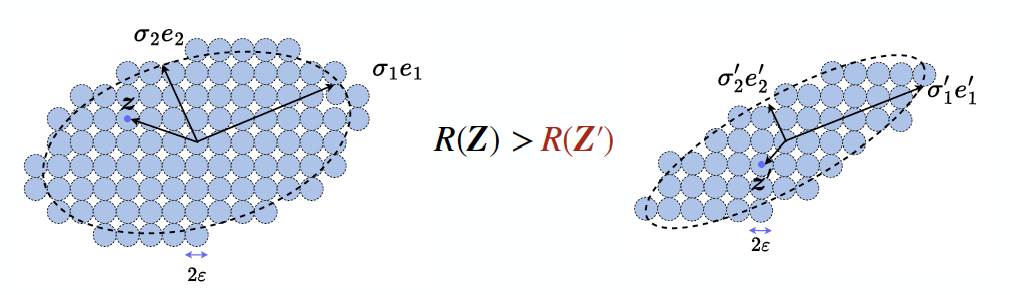
\includegraphics[width=\linewidth]{\toplevelprefix/chapters/chapter3/figs/Gaussian-compression.png}
	\caption{用 $\epsilon$-球覆盖由数据向量张成的区域。空间的体积越大,需要的球就越多,因此编码和枚举这些球所需的比特数就越多。每个实值向量 $\vx$ 都可以被编码为它落入的球的编号。}
	\label{fig:ball-packing}
\end{figure}

为了编码落入由 $\hat \x_i$ 张成的区域的向量,我们可以用半径为 $\epsilon$ 的不重叠的球来覆盖该区域,如图 \ref{fig:ball-packing} 所示。当由 $\hat \x_i$ 张成的区域的体积显著大于 $\epsilon$-球的体积时,我们需要覆盖该区域的球的总数约等于这两个体积的比值:
\begin{equation}
	\# \,\epsilon\mbox{-球} \approx \frac{\mbox{体积}(\hat \vx_i)}{\mbox{体积}(\vw_i)} = \sqrt{\det\left(\boldsymbol{I} + \frac{D}{N\epsilon^2} \X\X^\top  \right)}.
\end{equation}
如果我们用二进制数来标记感兴趣区域中的所有 $\epsilon$-球,那么所需的二进制比特总数就是 %\DP{suggest using notation \(R_{\eps}\) since the ``conditional'' notation will become overused in future.}
\begin{equation} 
	\cR_{\epsilon}(\X) \approx %\doteq 
	\log_2 (\# \,\epsilon\mbox{-球}) \approx R_{\epsilon}(\X) \doteq \frac{1}{2} \log \det \left(\boldsymbol{I} + \frac{D}{N\epsilon^2} \X\X^\top \right).
	\label{eqn:rate-Gaussian}
\end{equation}

\begin{example}
	图 \ref{fig:ball-packing} 展示了一个具有椭球形支撑的二维分布的例子——近似于一个二维高斯分布的支撑。该区域被大小为 $\epsilon$ 的小球覆盖。所有的球从 $1$ 编号到比如说 $n$。那么给定这个区域中的任何向量 $\x$,我们只需要确定它最接近哪个 $\epsilon$-球的中心,记作 $\operatorname{ball}_{\epsilon}(\x)$。为了记住 $\x$,我们只需要记住这个球的编号,这需要 $\log(n)$ 比特来存储。如果我们需要从这个编号解码 $\x$,我们只需取 $\hat \x$ 作为球的中心。这就产生了一个显式的编码和解码方案:
	\begin{equation}
		\x \longrightarrow \operatorname{ball}_{\epsilon}(\x) \longrightarrow \hat \x = \mbox{中心} \operatorname{ball}_{\epsilon}(\x).
	\end{equation}
	人们可以将这些球心称为编码方案的码本或字典中的“码字”。很容易看出,这个(有损)编码-解码方案的精度大约是球的半径 $\epsilon$。显然,$\cR_{\epsilon}(\Z)$ 是用这个编码方案编码每个向量 $\z$ 的球编号所需的平均比特数,因此可以称之为与该方案相关的{\em 编码率}。
\end{example}


从上述推导中,我们知道编码率 $\cR_{\epsilon}(\X)$ 是(近似)可以通过一个显式的编码(和解码)方案实现的。它有两个有趣的性质:
\begin{itemize}
	\item 首先,人们可能会注意到 $R_{\epsilon}(\X)$ 与高斯信源的率失真函数非常相似 \cite{Cover-Thomas}。事实上,当 $\epsilon$ 很小时,上述表达式是高斯信源率失真的一个很好的近似,正如 \cite{MaY2007-PAMI} 所指出的。
	\item 其次,如果假设数据 $\X$ 来自一个线性子空间,那么可以推导出相同的封闭形式编码率 $R_{\epsilon}(\X)$ 作为 \(\cR_{\epsilon}(\vX)\) 的近似。这可以通过适当地量化 $\X$ 的奇异值分解(SVD)$\X = \boldsymbol{U} \boldsymbol{\Sigma}\boldsymbol{V}^\top$ 并为由 $\boldsymbol{U}$ 张成的子空间中的向量构建一个有损编码方案来证明 \cite{MaY2007-PAMI}。
\end{itemize}
在我们的背景下,封闭形式的表达式 $R_{\epsilon}(\X)$ 是相当基础的:它是与为从高斯分布或线性子空间中抽取的数据设计的显式和自然的有损编码方案相关的编码率。正如我们将在下一章看到的,这个公式在理解深度神经网络的架构方面扮演着重要的角色。


\subsection{聚类低维高斯混合模型}
\label{sec:clustering-Gaussians}
正如我们之前讨论的,给定的数据集 $\X$ 通常具有低维的内在结构。因此,将其编码为一个普通的高斯分布将是非常冗余的。如果我们能识别出 $\X$ 中的那些内在结构,我们就可以设计出更好的编码方案,从而得到更低的编码率。或者等价地说,用于编码这样的 $\X$ 的码字可以被压缩。我们将看到,压缩提供了一种统一的可计算的方法来识别这些结构。在本节中,我们将用最基本的低维结构族来演示这个重要的思想:低维高斯或子空间的混合。

\begin{example}
	图 \ref{fig:two-subspaces} 展示了一个例子,其中数据 $\X$ 分布在两个子空间(或低维高斯)周围。如果将它们视为一个单一的高斯分布并一起编码,相关的离散(有损)码本,由所有蓝色球表示,显然是非常冗余的。我们可以尝试识别两个子空间的位置,记为 $S_1$ 和 $S_2$,并设计一个只覆盖这两个子空间的码本,即绿色球。如果我们能正确地将数据 $\X$ 中的样本划分到两个子空间中:$\X = [\X_1, \X_2]\bm \Pi$,其中 $\X_1 \in S_1$ 且 $\X_2 \in S_2$,$\bm \Pi$ 表示一个置换矩阵,那么数据的最终编码率将会低得多。这为数据提供了一个更简约,因此更理想的表示。
\end{example}

\begin{figure}
	\centering
	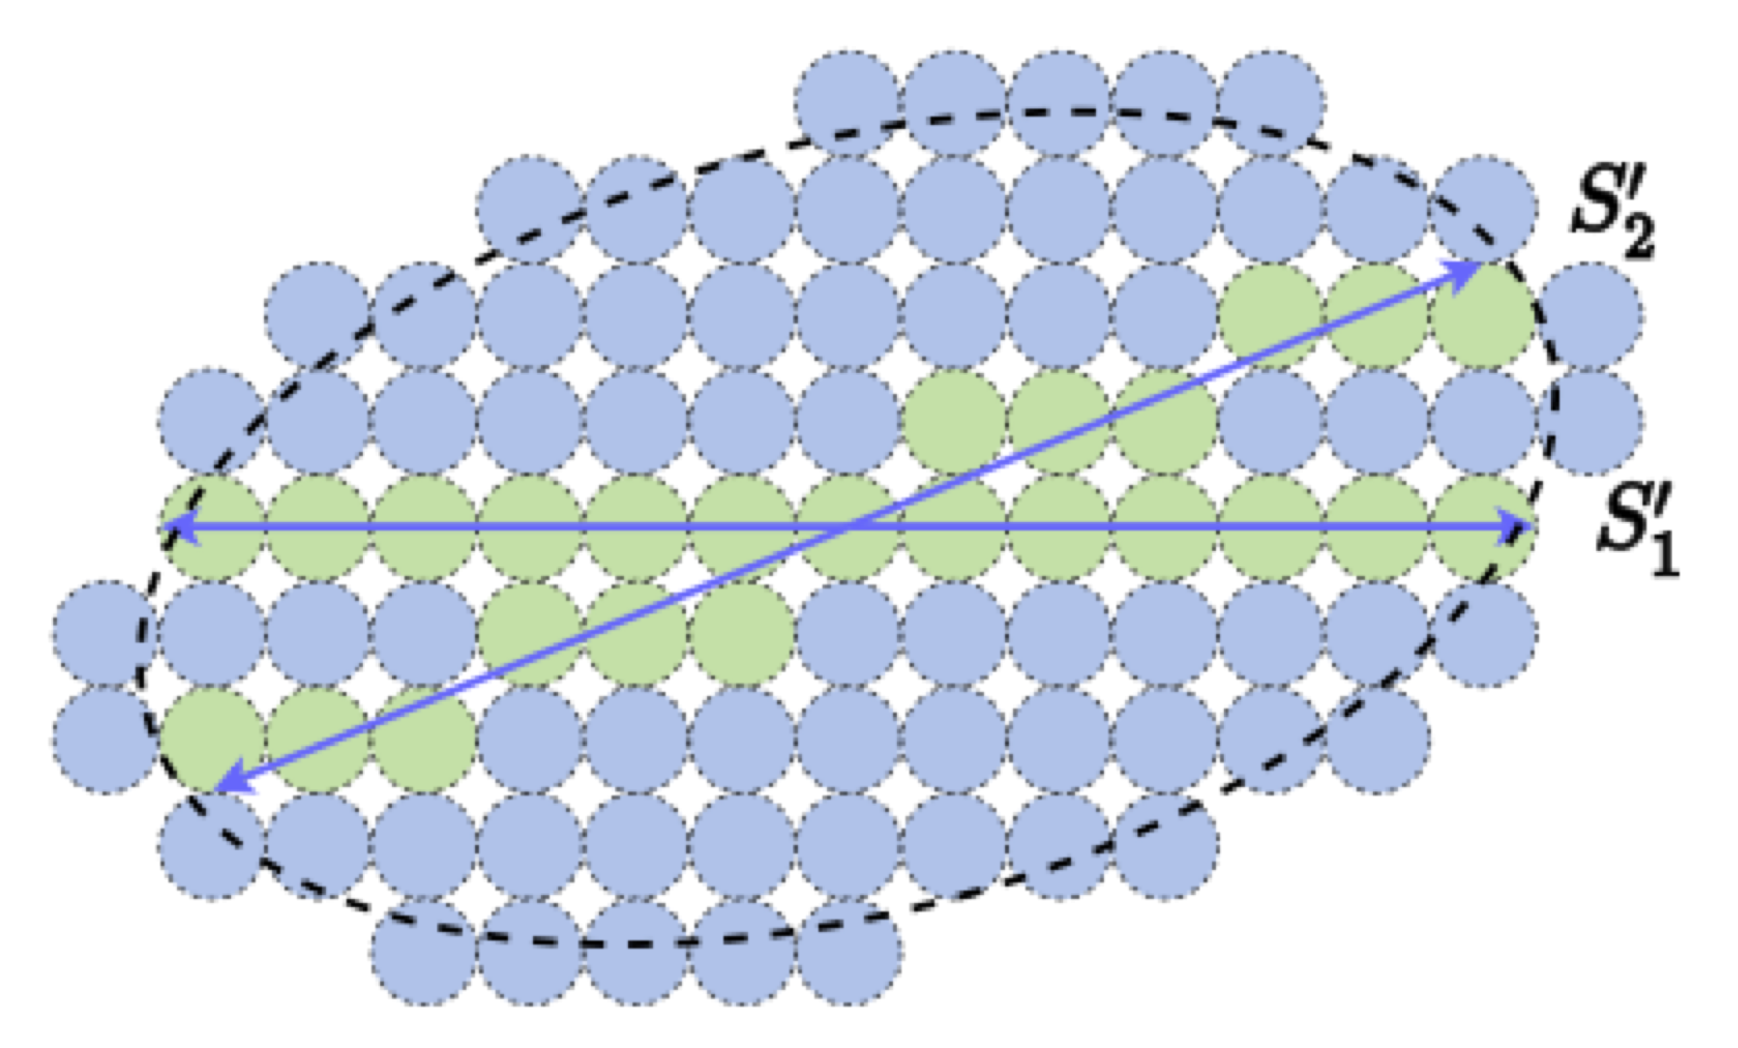
\includegraphics[width=0.5\linewidth]{\toplevelprefix/chapters/chapter3/figs/Two-subspaces.png}
	\caption{两种有损编码方案的比较,用于分布在两个子空间周围的数据。一种是用(蓝色)$\epsilon$-球填充由两个子空间张成的整个空间;另一种是只在两个子空间周围的邻域内填充球。后者显然有一个小得多的码本,并且对于子空间上的样本,其编码率要低得多。}
	\label{fig:two-subspaces}
\end{figure}

所以,更一般地说,如果数据是从任何子空间或低维高斯的混合体中抽取的,那么识别这些成分并根据这些成分的内在维度来编码数据将是可取的。事实证明,假设数据是从低维高斯的混合体中抽取的,我们并不会损失太多的一般性。这是因为高斯的混合体可以很好地近似大多数一般的分布 \cite{borkar2016gaussian}。

\paragraph{聚类问题。}
现在对于这个特定的分布族,我们如何能有效地从一组样本中识别出那些低维成分
\begin{equation}
	\X = \left[\x_1, \x_2, \ldots, \x_N\right],
\end{equation}
这些样本是从它们中抽取的?换句话说,给定整个数据集 $\X$,我们想要将其划分或聚类成多个,比如说 $K$ 个子集:
\begin{equation}
	\X\bm \Pi = [\X_1, \X_2, \dots, \X_K],
\end{equation}
其中每个子集由仅从一个低维高斯或子空间中抽取的样本组成,而 $\bm \Pi$ 是一个置换矩阵,用于指示划分的成员关系。请注意,根据情况,划分可以是确定性的,也可以是概率性的。正如 \cite{ma2007segmentation} 中所示,对于高斯混合模型,概率性划分不会导致更低的编码率。因此,为简单起见,我们这里只考虑确定性划分。

\paragraph{通过有损压缩进行聚类。}
解决上述聚类问题的主要困难在于,我们通常不知道聚类的数量 $K$,也不知道每个成分的维度。对这个聚类问题的研究有很长的历史。教科书 \cite{GPCA} 系统而全面地涵盖了解决这个问题的不同方法。为了找到解决这个问题的有效方法,我们首先需要理解和澄清我们为什么要聚类。换句话说,与不聚类相比,我们从聚类数据中究竟能得到什么?我们如何衡量这种增益?从数据压缩的角度来看,一个正确的聚类应该能导出一个更高效的编码(和解码)方案。

对于任何给定的数据集 $\X$,已经有两个明显的编码方案作为基准。它们代表了两种极端的数据编码方式:
\begin{itemize}
	\item 简单地将所有样本视为从一个单一的高斯分布中抽取的。相关的编码率,如前所述,由下式给出:
	      \begin{equation}
		      \cR_{\epsilon}(\vX) \approx R_{\epsilon}(\X) = \frac{1}{2} \log \det \left(\boldsymbol{I} + \frac{D}{N\epsilon^2} \X\X^\top \right).
	      \end{equation}
	\item 简单地通过为每个样本分配一个不同的编号来分别记住所有样本。编码率将是:
	      \begin{equation}
		      \cR_0(\X) = \log(N).
	      \end{equation}
\end{itemize}


请注意,对于某些(极端的)量化误差 $\epsilon$ 的选择,这两种编码方案中的任何一种都可能成为“最优”解:
\begin{enumerate}
	\item {\em 懒惰区域}:如果我们选择 $\epsilon$ 极大,$\X$ 中的所有样本都可以被一个单独的球覆盖。此时的率是 $\lim_{\epsilon \rightarrow \infty} \cR_\epsilon \rightarrow \frac{1}{2}\log\det (\boldsymbol{I}) = 0$。
	\item {\em 记忆区域}:如果 $\epsilon$ 极小,$\X$ 中的每个样本都被一个不同的 $\epsilon$-球覆盖,因此总共有 $N$ 个。此时的率是 $\lim_{\epsilon \rightarrow 0} \cR_\epsilon \rightarrow \log(N)$。
\end{enumerate}
请注意,第一种方案对应于人们根本不关心分布的任何有趣特性的情况。人们不想为任何有信息量的内容花费任何比特。我们称之为“懒惰区域”。第二种方案对应于人们希望以极高的精度解码每个样本的情况。所以人们最好“记住”每个样本。我们称之为“记忆区域”。
\begin{figure}
	\centering
	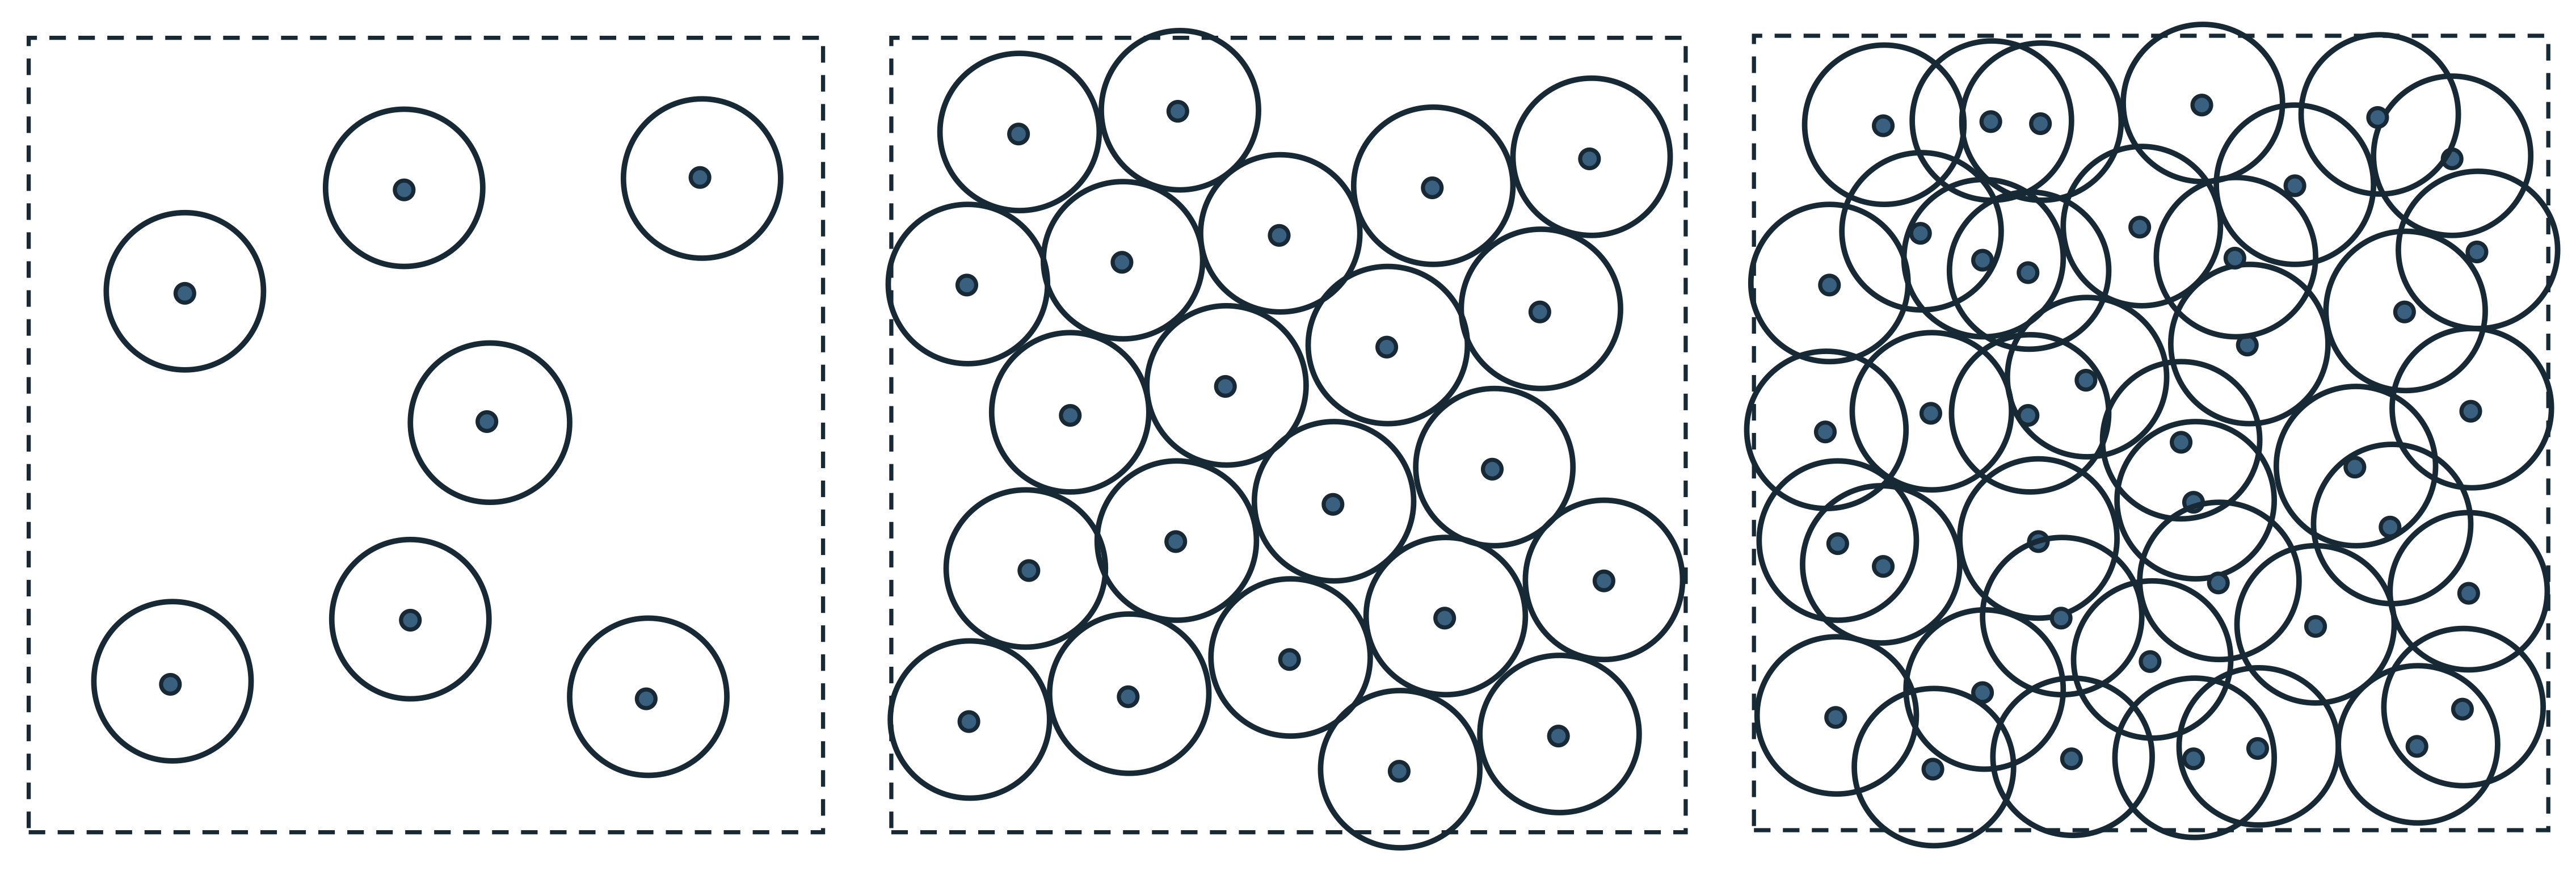
\includegraphics[width=0.9\linewidth]{\toplevelprefix/chapters/chapter3/figs/circle-packing.png}
	\caption{在二维平面上的一些随机样本。考虑为每个样本分配一个以该样本为中心的 $\epsilon$-圆盘。样本的密度从左到右增加。}
	\label{fig:circle-packing}
\end{figure}
\begin{example}
	为了看看记忆区域在什么时候是可取的,让我们考虑在二维平面的一个单位区域内随机分布的一些样本,比如说 $N$ 个。\footnote{比如说这些点是由一个密度为每单位面积 $N$ 个点的泊松过程抽取的。} 想象一下,我们试图设计一个固定量化误差 $\epsilon$ 的有损编码方案。这等同于在每个样本周围放置一个 $\epsilon$-圆盘,如图 \ref{fig:circle-packing} 所示。当 $N$ 很小时,所有圆盘相互重叠的几率为零。在这种情况下,一个大小为 $N$ 的码本是必要且最优的。当 $N$ 或密度达到某个临界值 $N_c$ 时,所有圆盘很可能开始重叠并连接成一个覆盖整个平面的聚类——这种现象被称为连续“逾渗” \cite{Gilbert-1961,Mertens-Moore-2012}。当 $N$ 变得大于这个值时,圆盘会严重重叠。$N$ 个圆盘的数量变得非常冗余,因为我们只想以给定的精度 $\epsilon$ 编码平面上的点。覆盖所有样本所需的圆盘数量远小于 $N$。\footnote{事实上,有高效的算法可以找到这样的覆盖 \cite{Booth-2001}。}
\end{example}

懒惰区域和记忆区域都有些微不足道,也许在理论上或实践上都没有什么意义。当用于编码从具有{\em 紧凑且低维支撑}的分布中抽取的大量样本时,这两种方案都远非最优。有趣的区域存在于这两者之间。
\begin{example}
	\begin{figure}[t]
		\centering
		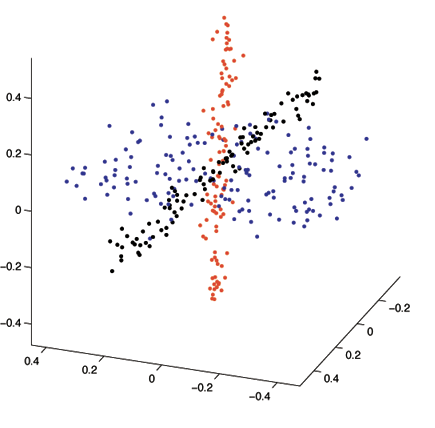
\includegraphics[width=0.4\linewidth]{\toplevelprefix/chapters/chapter3/figs/Two-lines-and-plane.png}
		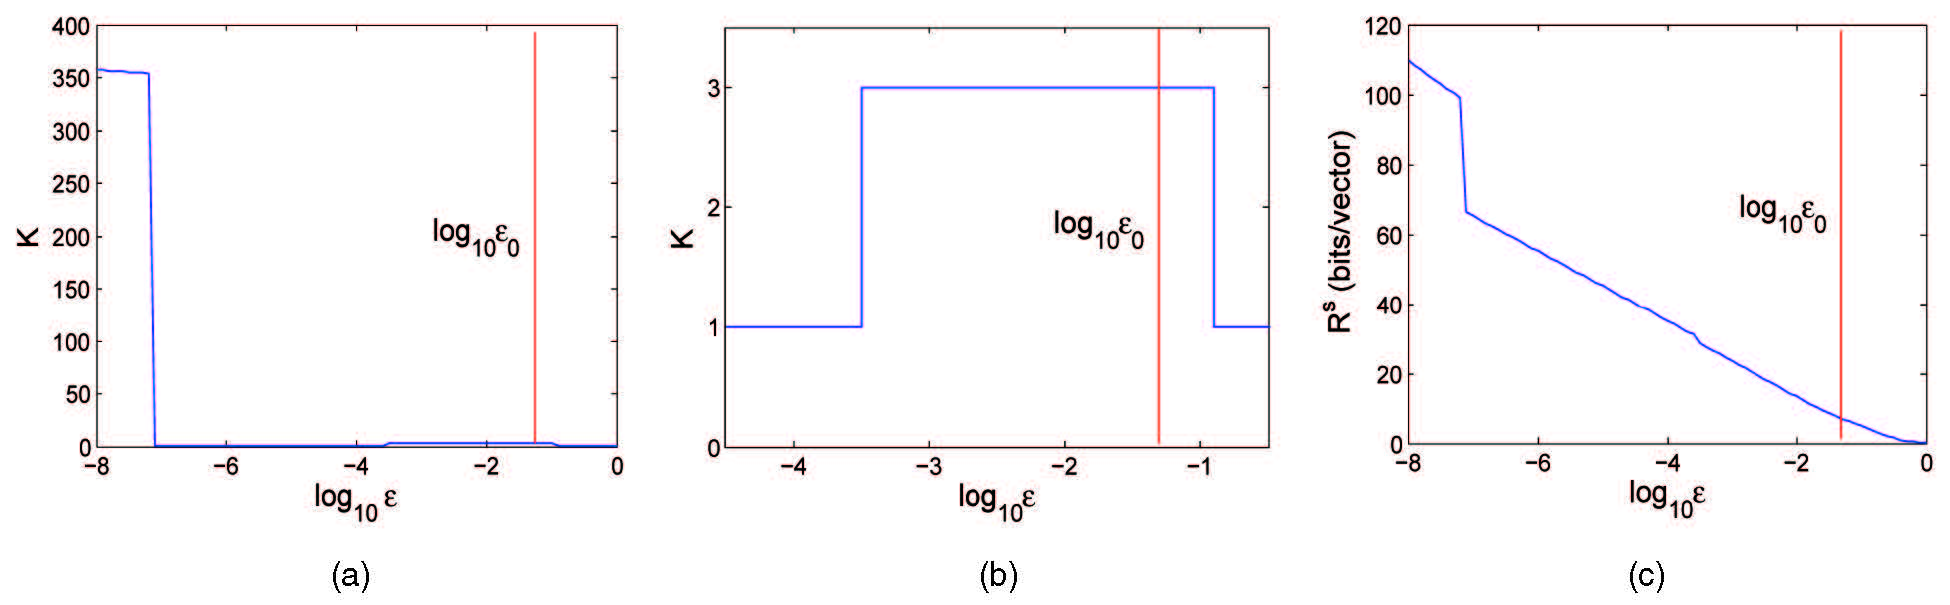
\includegraphics[width=0.9\linewidth]{\toplevelprefix/chapters/chapter3/figs/Coding-Rate.jpg}
		\caption{上图:从 $\mathbb{R}^3$ 中的两条线和一个平面抽取的 358 个带噪声的样本。下图:改变 $\epsilon$ 对聚类结果和编码率的影响。红线标记了添加到样本中的高斯噪声的方差 $\epsilon_0$。}
		\label{fig:two-lines-and-plane}
		\label{fig:two-lines-and-plane-epsilon}
	\end{figure}
	图 \ref{fig:two-lines-and-plane} 展示了一个例子,其中带噪声的样本是从 $\mathbb{R}^3$ 中的两条线和一个平面抽取的。正如我们从右侧的图 (c) 中注意到的,随着我们增加 $\epsilon$,最优编码率单调递减,这与率失真函数的性质相符。图 (a) 和 (b) 显示,当将 $\epsilon$ 从非常小(接近零)变化到非常大(趋于无穷)时,当编码率最小时的最优聚类数。我们可以清楚地看到图两端的懒惰区域和记忆区域。但人们也可以在图 (b) 中注意到,当选择的量化误差 $\epsilon$ 围绕真实噪声方差 $\epsilon_0$ 的水平时,最优聚类数是“正确的”数字三,代表两个平面和一个子空间。我们非正式地将这个中间区域称为“泛化区域”。请注意,在这些区域之间发生了急剧的相变。\footnote{到目前为止,据我们所知,对于这些相变行为还没有严格的理论证明。}
\end{example}


从上面的讨论和例子中,我们看到,当量化误差相对于样本密度\footnote{或者样本密度相对于量化误差}在一个合适的范围内时,最小化有损编码率将使我们能够揭示采样数据的底层(低维)分布。{\em 因此,最初作为实用性选择的量化,似乎对于从其有限样本的经验分布中学习一个连续分布变得必要。} 尽管解释这种现象的严格理论仍然难以捉摸,但在这里,为了学习的目的,我们关心的是如何利用这种现象来设计能够找到正确分布的算法。

让我们用图 \ref{fig:two-subspaces} 中所示的简单例子来说明基本思想。如果能将 $\X$ 中的所有样本划分成 $\X_1$ 和 $\X_2$ 两个聚类,分别有 $N_1$ 和 $N_2$ 个样本,那么相关的编码率将是\footnote{我们这里忽略了编码每个样本成员关系所需的一些开销比特,比如说通过霍夫曼编码。}
\begin{equation}
	R_{\epsilon}^c(\X\mid \boldsymbol{\Pi}) = \frac{N_1}{N}R_{\epsilon}(\X_1) + \frac{N_2}{N}R_{\epsilon}(\X_2),
\end{equation}
其中我们用 $\boldsymbol{\Pi}$ 来表示划分的成员关系。如果划分尊重分布的低维结构,在这种情况下 $\X_1$ 和 $\X_2$ 分别属于两个子空间,那么最终的编码率应该显著小于上述两个基本方案:
\begin{equation}
	R_{\epsilon}^c(\X \mid \boldsymbol{\Pi}) \ll R_{\epsilon}(\X), \quad     R_{\epsilon}^c(\X \mid \boldsymbol{\Pi}) \ll R_0(\X).
\end{equation}
总的来说,我们可以将聚类问题转化为一个最小化编码率的优化问题:
\begin{equation}
	\min_{\boldsymbol{\Pi}}  \bc{ R_{\epsilon}^c(\X \mid \boldsymbol{\Pi})
	\doteq \sum_{k=1}^K \frac{N_k}{N}R_{\epsilon}(\X_k)}.
\end{equation}

\paragraph{聚类的优化策略。}
剩下的问题是我们如何优化上述编码率目标来找到最优的聚类。对于这个目标,有三种自然的方法:
\begin{enumerate}
	\item 我们可以从整个集合 $\X$ 作为一个单一的聚类开始(即懒惰区域),然后(比如说随机地)搜索将其划分,以期得到更小的编码率。
	\item 相反,我们可以从每个样本 $\x_i$ 作为其自身的聚类开始(即记忆区域),然后搜索合并那些能导致更小编码率的聚类。
	\item 或者,如果我们能将成员关系 $\boldsymbol{\Pi}$ 表示为一些连续参数,我们可以使用诸如梯度下降(GD)之类的优化方法。
\end{enumerate}
第一种方法在计算上不那么吸引人,因为需要尝试的可能划分数量在样本数量上是指数级的。例如,将 $\X$ 划分成两个大小相等的子集的数量是 $N \choose N/2$,当 $N$ 变大时,这个数量会爆炸式增长。我们将在下一章 \ref{ch:representation} 中探讨第三种方法。在那里,我们将看到深度神经网络,特别是 Transformer,的角色如何与编码率目标联系起来。



第二种方法最初是在 \cite{ma2007segmentation} 的工作中提出的。它展示了能够高效地(比如说用解析形式)评估编码率的好处。有了它,数据的(低维)聚类可以通过最小化编码长度(MCL)的原则相当高效和有效地找到。请注意,对于一个有 $N_k$ 个样本的聚类 $\X_k$,编码 $\X_k$ 中所有样本所需的二进制比特长度由下式给出:\footnote{事实上,编码长度的一个更精确的估计是 $L(\X_k) = (N_k+D) R_\epsilon(\X_k)$,其中额外的比特用于编码子空间的基 \cite{ma2007segmentation}。为简单起见,我们在此省略了这个开销。}
\begin{equation}
	L(\X_k) = N_k R_\epsilon(\X_k).
\end{equation}
如果我们有两个聚类 $\X_k$ 和 $\X_l$,如果我们想将样本编码为两个独立的聚类,所需的二进制比特长度是
\begin{equation*}
	L^c(\X_k, \X_l) = N_k R_\epsilon(\X_k) + N_l R_\epsilon(\X_l) - N_k \log\frac{N_k}{N_k + N_l} - N_l \log\frac{N_l}{N_k + N_l}.
\end{equation*}
最后两项是根据霍夫曼编码对样本的成员关系进行编码所需的比特数。

那么,给定任意两个独立的聚类 $\X_1$ 和 $\X_2$,我们可以根据两个编码长度的差值来决定是否合并它们:
\begin{equation}
	L(\X_k \cup \X_l) - L^c(\X_k, \X_l)
\end{equation}
是正还是负,其中 $\X_k \cup \X_l$ 表示 $\bm X_k$ 和 $\bm X_l$ 中样本集合的并集。如果是负的,意味着如果我们将这两个聚类合并成一个,编码长度会变小。这个简单的事实导致了 \cite{ma2007segmentation} 提出的以下聚类算法:
\begin{algorithm}[!htbp]
	\caption{编码长度的成对最速下降法}\label{alg:steepest_descent_coding_length}
	\begin{algorithmic}
		\Require{\(N\) 个数据点 \(\{\vx_{i}\}_{i = 1}^{N}\)}
		\Ensure{一个聚类集合 \(\cC\)}

		\Procedure{PairwiseSteepestDescentOfCodingLength}{$\{\vx_{i}\}_{i = 1}^{N}$}
		\State{\(\cC \gets \{\{\bm x_{i}\}\}_{i = 1}^{N}\)} \Comment{初始化 \(N\) 个聚类 \(\vX_{k}\),每个聚类包含一个元素}
		\While{\(\abs{\cC} > 1\)}
		\If{\(\displaystyle \min_{\vX_{k}, \vX_{l} \in \cC}[L(\vX_{k} \cup \vX_{l}) -L^{c}(\vX_{k}, \vX_{l})] \geq 0\)} \Comment{如果任何合并都不能节省比特}
		\State{\Return{\(\cC\)}} \Comment{提前返回 \(\cC\) 并退出}
		\Else
		\State{\(\displaystyle \vX_{k^{\ast}}, \vX_{l^{\ast}} \gets \argmin_{\vX_{k}, \vX_{l} \in \cC}[L(\vX_{k} \cup \vX_{l}) - L^{c}(\vX_{k}, \vX_{l})]\)} \Comment{合并节省最多比特的聚类}
		\State{\(\displaystyle \cC \gets [\cC \setminus \{\vX_{k^{\ast}}, \vX_{l^{\ast}}\}] \cup \{\vX_{k^{\ast}} \cup \vX_{l^{\ast}}\}\)} \Comment{移除未合并的聚类并加回合并后的聚类}
		\EndIf
		\EndWhile
		\State{\Return{\(\cC\)}}  \Comment{如果所有合并都有节省,则返回一个聚类}
		\EndProcedure
	\end{algorithmic}
\end{algorithm}

请注意,该算法是易于处理的,因为(成对)比较和合并的总数约为 $O(N^2\log N)$。然而,由于其贪婪的性质,没有理论保证该过程会收敛到全局最优的聚类解。尽管如此,正如 \cite{ma2007segmentation} 中所报道的,在实践中,这个看似简单的算法效果非常好。图 \ref{fig:two-lines-and-plane} 中绘制的聚类结果实际上就是由这个算法计算的。

%\subsection{Applications of Subspace  Clustering}

\begin{example}[图像分割]\label{eg:image-segmentation} 上述编码长度的度量和相关的聚类算法假设数据分布是(低维)高斯的混合。尽管这看起来有些理想化,但在模型(近似)有效的情况下,该度量和算法已经可以非常有用甚至强大。

	例如,一幅自然图像通常由多个具有近乎同质纹理的区域组成。如果我们从每个区域中取许多小窗口,它们应该类似于从一个(低维)高斯分布中抽取的样本,如图 \ref{fig:image-patch} 所示。图 \ref{fig:image-segmentation} 显示了将上述聚类算法直接应用于图像块的图像分割结果。有关将算法定制到图像分割问题的更多技术细节,可以在 \cite{Mobahi-IJCV2011} 中找到。
\end{example}


\begin{figure}
	\centering
	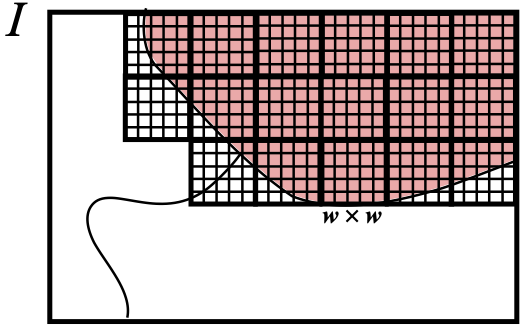
\includegraphics[width=0.4\linewidth]{\toplevelprefix/chapters/chapter3/figs/image-segmentation-tiles.png}
	\caption{大小为 $w\times w$ 像素的图像块。}
	\label{fig:image-patch}
\end{figure}

\begin{figure}[th]
	\centering
	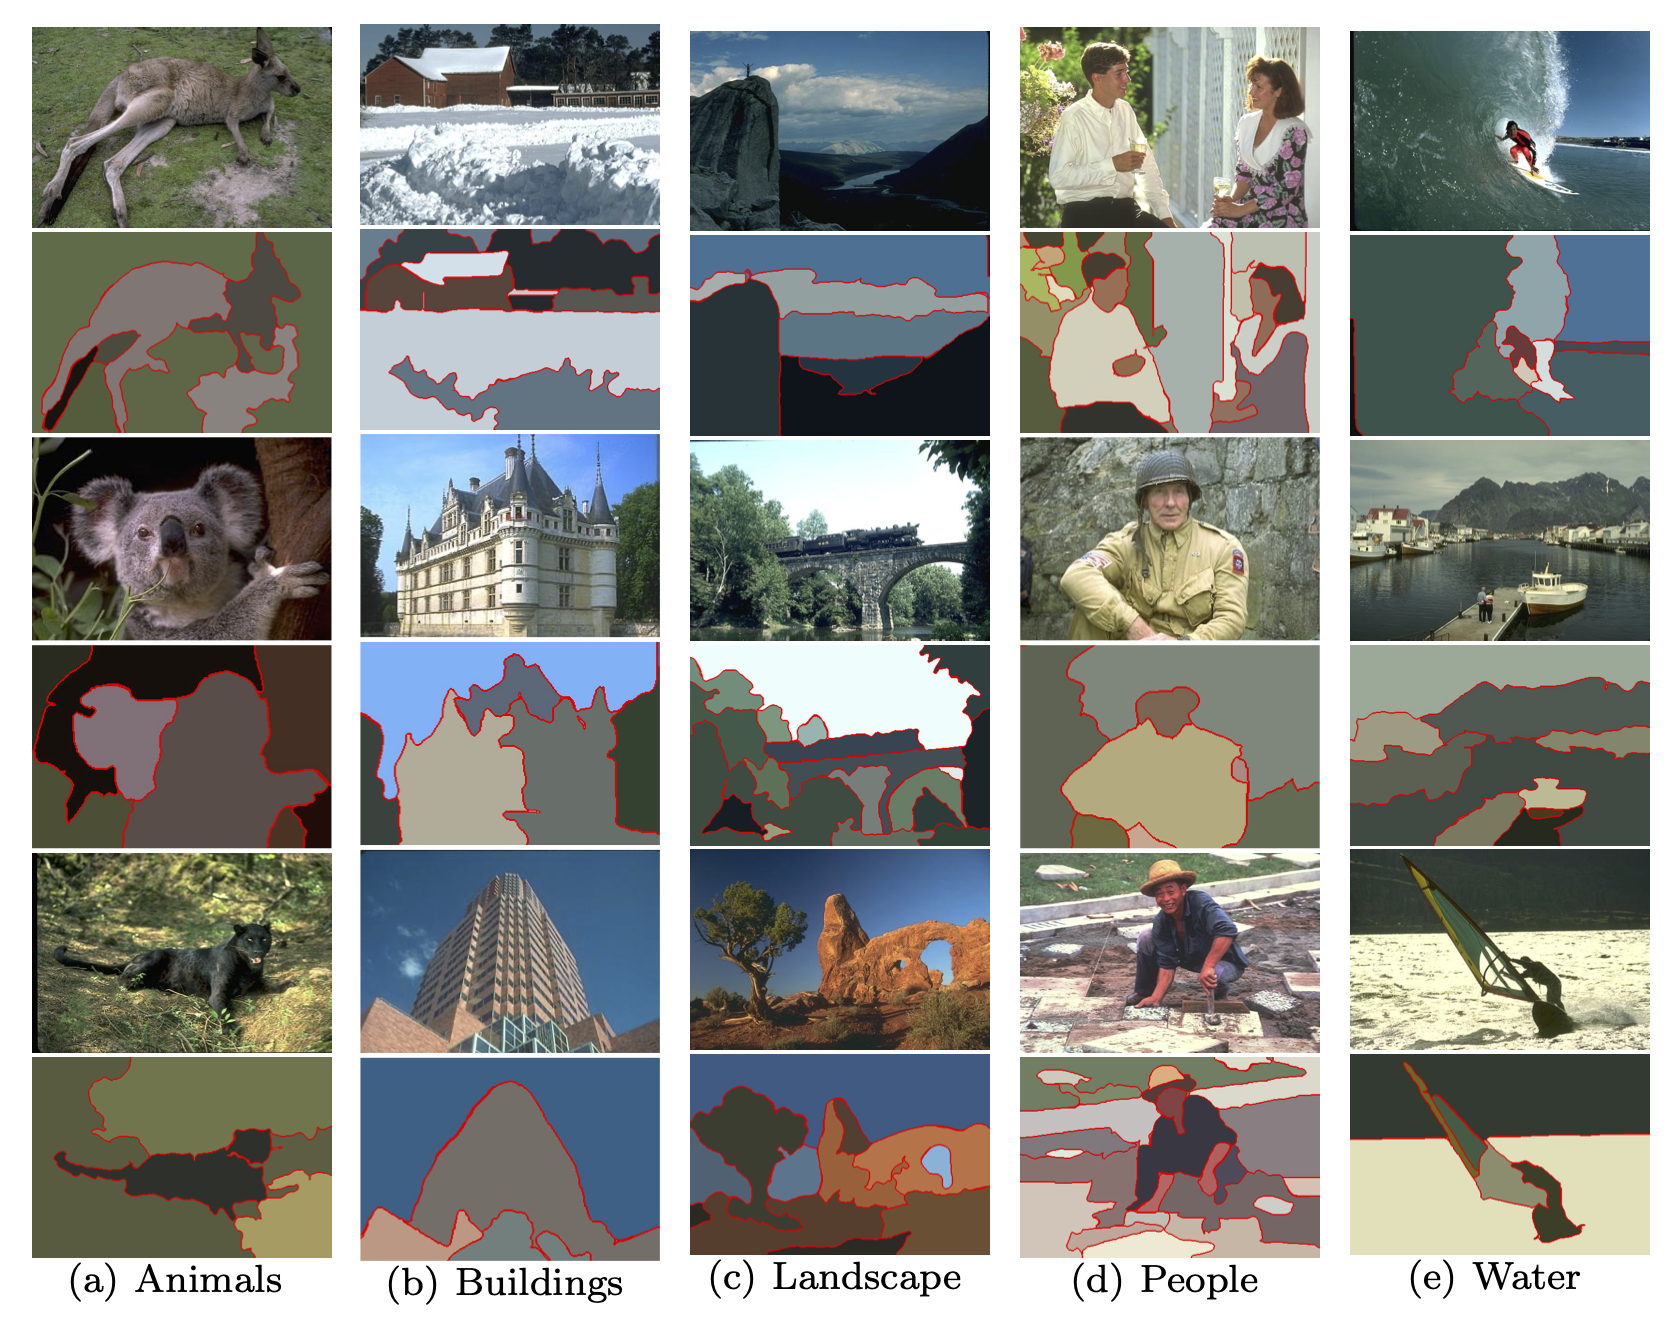
\includegraphics[width=0.8\linewidth]{\toplevelprefix/chapters/chapter3/figs/image-segmentation.png}
	\caption{基于聚类算法应用于图像块的分割结果。}
	\label{fig:image-segmentation}
\end{figure}

\section{最大化信息增益}
\label{sec:chap4-representation-learning-problem}

% \yaodong{TODO: Connect representation properties defined in Chapter 2. (suggested by Druv)}

% \yaodong{TODO: cut the citations to the ``Notes'' part in the later of the chapter.}

%\pw{add some sentences to connect!}

到目前为止,在本章中,我们已经讨论了如何通过压缩的原则来识别具有低维结构的分布。正如我们从前两节所看到的,计算压缩可以通过去噪操作或聚类来实现。图 \ref{fig:Gaussian-Subspaces} 用我们最喜欢的例子阐述了这个概念。
\begin{figure}[t]
    \centering
    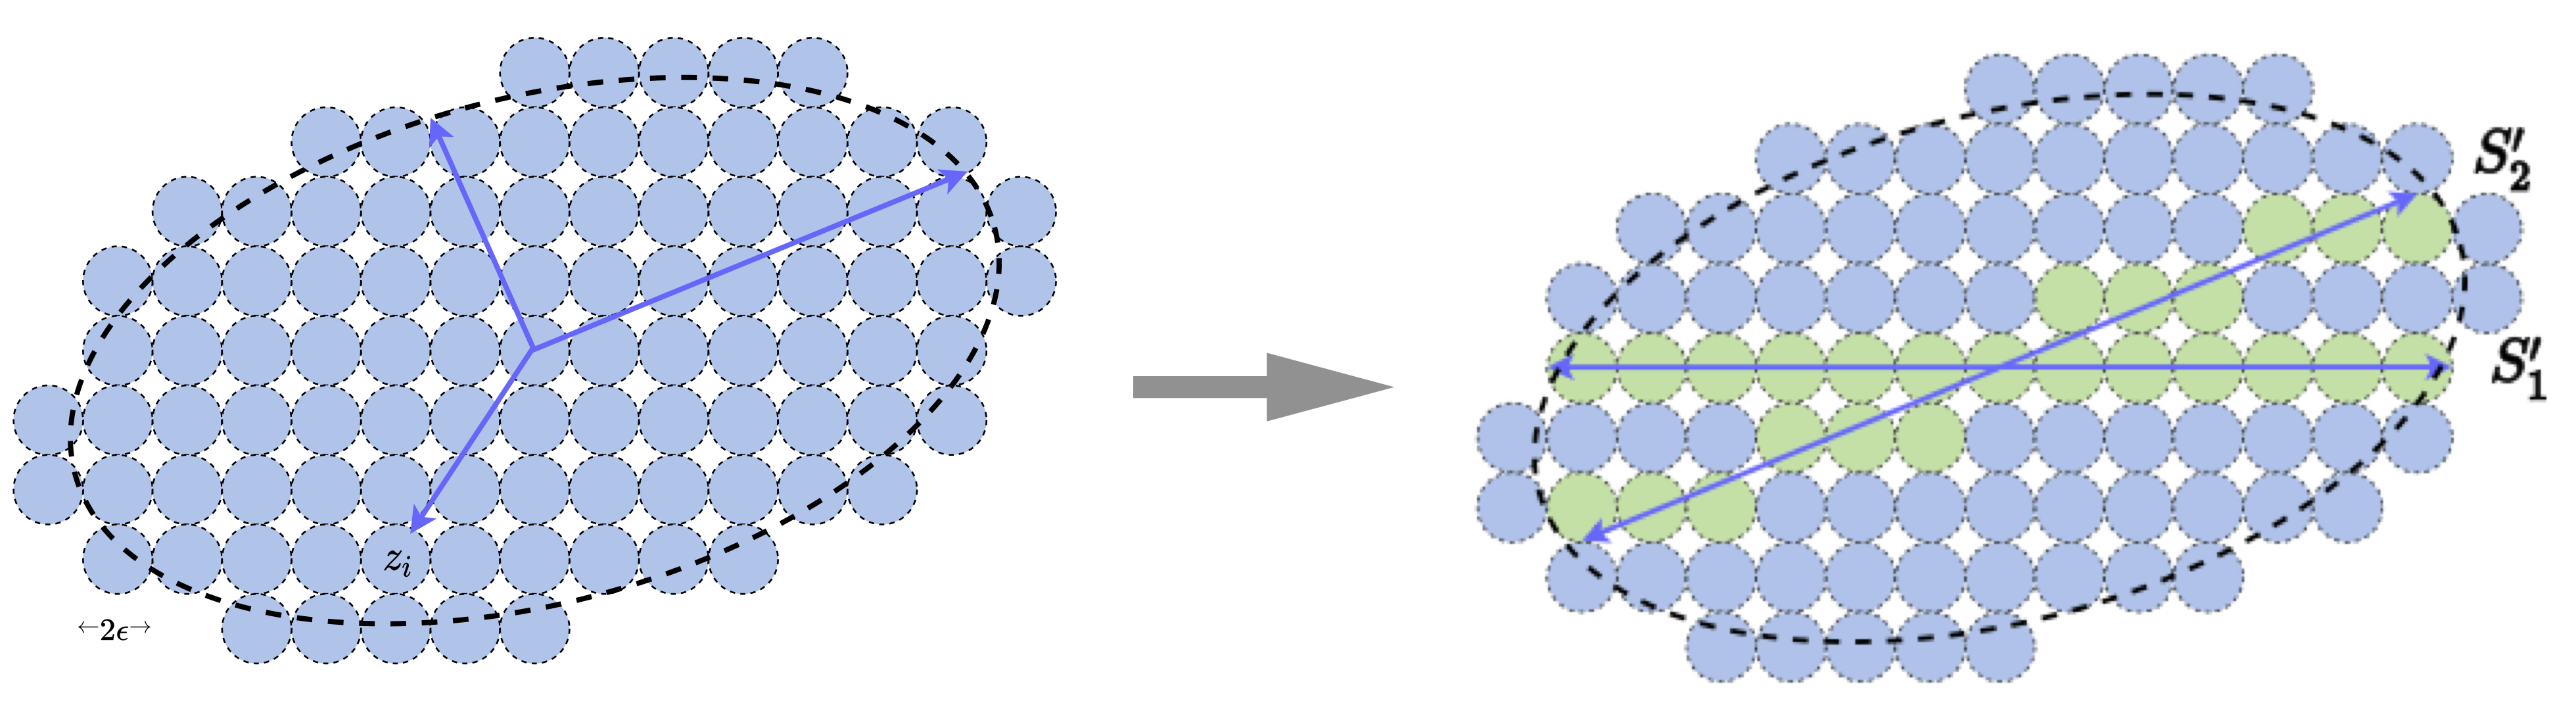
\includegraphics[width=0.8\linewidth]{\toplevelprefix/chapters/chapter3/figs/Gaussian-Subspaces.png}
    \caption{通过去噪或聚类,从一个通用的随机高斯分布(右)开始,识别一个具有两个子空间的低维分布(左)。}
    \label{fig:Gaussian-Subspaces}
\end{figure}
当然,识别数据分布的最终目标是利用它来促进后续任务,如分割、分类或(图像)生成。因此,最终的分布如何被“表示”对于如何高效、有效地检索和利用与这些后续任务相关的信息至关重要。这自然引出了一个基本问题:{\em 是什么让一个表示对于下游使用真正“好”?} 在下文中,我们将探讨一个有意义和有用的表示应该具备的基本属性,以及如何通过最大化信息增益来明确地刻画和追求这些属性。

% In recent years, deep learning has seen tremendous empirical success in processing
% and modeling massive amounts of high-dimensional and multi-modal data. Much of this success has been attributed to deep networks' ability in effectively learning  ``good representations'' that facilitate many downstream tasks, e.g., classification, recognition and segmentation, and generation of visual data.

\paragraph{如何衡量表示的好坏。}
% To state the common problem behind all these practices more formally, 
可以将给定的数据集视为一个随机向量 $\x$ 的样本,该向量在某个高维空间(比如 $\mathbb{R}^D$)中具有一定的分布。通常,$\x$ 的分布的内在维度远低于环境空间。一般来说,{\em 学习一个表示} 指的是学习一个连续映射,比如说 $f(\cdot)$,它将 $\x$ 转换到另一个(通常是低维的)空间(比如 $\mathbb{R}^d$,其中 $d < D$)中的一个所谓的{\em 特征向量} $\z$。希望通过这样的映射
\begin{equation}
	\x \in \mathbb{R}^D \xrightarrow{\hspace{2mm} f(\x)\hspace{2mm}} \z  \in \mathbb{R}^d,
	\label{eqn:chap4-1-encoding}
\end{equation}
$\x$ 的低维内在结构被识别并以一种更紧凑和结构化的方式由 $\z$ 表示,以便于后续任务,如分类或生成。特征 $\z$ 可以被看作是原始数据 $\x$ 的一个(学习到的)紧凑编码,所以映射 $f$ 也被称为\textit{编码器}。
表示学习的基本问题是
\begin{center}
	\noindent{\em 什么是衡量表示好坏的原则性和有效的方法?}
\end{center}

从概念上讲,一个表示 $\z$ 的质量取决于它如何为后续任务识别出 $\x$ 最相关和最充分的信息,以及它如何有效地表示这些信息。
很长一段时间以来,人们相信并认为,学习到的特征表示的“充分性”或“好坏”应该根据特定的任务来定义。例如,在分类问题中,$\z$ 只需要足以预测类别标签 $\y$。下面,让我们从经典的图像分类问题开始,论证为什么这种任务特定的“表示”概念是有限的,需要被推广。

%To understand the role of deep learning or deep networks in this type of representation learning, \cite{Tishby-ITW2015} proposed the \textit{information bottleneck} framework, which suggests that a measure of feature goodness is to maximize the mutual information between $\z$ and $\y$ while minimizing the mutual information between $\z$ and $\x$.

% Nevertheless, in recent years the predominant practice has been to learn first a \textit{task-agnostic} representation by pre-training a large deep neural network, in some cases known as a \textit{foundation model} \cite{Bommasani2021-vm}.
% The so-learned representation can subsequently be fine-tuned for multiple specific tasks.
% This has been shown to be more effective and efficient for many practical tasks across diverse data modalities, including speech, language, and natural images.
% Notice that representation learning in this context is different from that for a specific task, where $\z$ only needs to be good enough for predicting a specific $\y$. In a task-agnostic setting, the learned representation $\z$ needs to encode \textit{almost all essential information about the distribution of the data $\x$}. That is, the learned representation $\z$ not only is a more compact and structured representation for the intrinsic structures of $\x$, but can also recover $\x$ to a certain degree of faithfulness.
% Hence, it is natural to ask, in the task-agnostic context, what a principled measure of goodness for a learned (feature) representation should be.
% As we know, in recent practice of learning task-agnostic representations, one type of deep architectures, known as transformers \cite{vaswani2017attention}, have emerged as an almost universal choice for the backbone of deep networks, for either discriminative or generative tasks, from language to vision.
% %We will provide more details on how to derive transformer-like architecture via a white-box approach in Section~\ref{sec:chap4-white-box-transformer}.
% As we will see in this chapter, clarifying the principled measure for feature goodness is also the key to fully understand why a transformer-like architecture is suitable for task-agnostic pretraining, as well as to reveal the precise role and function of each layer in transformer-like deep networks.


% \subsection{Principles and Objectives for Representation Learning}


% TODO: compression and sparsity.

% \subsection{Deep Network Architectures: Nonlinear to Linear}


% \section{White-box Deep Networks via Unrolling}\label{sec:chap4-white-box-model-via-unrolling}

% \subsection{LISTA - Sparsity}

% \subsection{ReduNet - Compression}

% \subsection{CRATE - Compression \& Sparsity}



\subsection{线性判别表示}\label{subsec:LDR}
%{\color{red} Outline: Introducing and formulating the principle of {\em information gain} or {\em rate reduction}. Transform the data distribution to maximize information gain. More specifically rate reduction in the important case of mixture of low-rank Gaussians.}

假设 $\bm{x} \in \mathbb{R}^D$ 是一个从 $K$ 个(成分)分布 $\mathcal{D} = \{\mathcal{D}_k\}_{k=1}^K$ 的混合体中抽取的随机向量。给定随机向量 $\bm x$ 的一组有限的独立同分布样本 $\X = [\x_1, \x_2, \ldots, \x_N] \in \Re^{D\times N}$,我们{\em 寻求一个好的表示},通过一个连续映射 $f(\x): \mathbb{R}^D \rightarrow \mathbb{R}^d$ 来捕捉 $\x$ 的内在结构,并最好地促进后续的分类任务。\footnote{分类是深度学习展示其初步成功,并引发对深度网络爆炸性兴趣的领域。尽管我们的研究集中在分类上,我们相信这些思想和原则可以自然地推广到其他设置,如回归。} 为了简化学习分布 $\mathcal{D}$ 的任务,在流行的监督分类设置中,为每个样本 $\x_i$ 提供一个真实的类别标签(或每个类别的码字),通常由一个独热向量 $\y_i \in \mathbb{R}^K$ 表示。

 

% Given a random vector $\bm{x} \in \mathbb{R}^D$ that is drawn from a mixture of $k$ (component) distributions  $\mathcal{D} = \{\mathcal{D}^j\}_{j=1}^k$, one of the most fundamental problems is how to effectively and efficiently {\em learn the underlying distribution} from a finite set of i.i.d. samples, say $\X = [\x_1, \x_2, \ldots, \x_N] \in \Re^{D\times N}$. 
% To this end, we {\em seek a good representation}  through a continuous mapping $f(\x): \mathbb{R}^D \rightarrow \mathbb{R}^d$ that captures intrinsic structures of $\x$ and best facilitates the subsequent classification task.\footnote{Classification is where deep learning demonstrated the initial success that has catalyzed the explosive interest in deep networks. Although our study focuses on classification, we believe the ideas and principles can be naturally generalized to other settings, such as regression.} 

\paragraph{通过交叉熵编码类别信息。}  大量研究表明,对于许多实际数据集(例如,图像、音频和自然语言),从数据 $\bm{x}$ 到其类别标签 $\bm{y}$ 的(编码)映射可以通过训练一个深度网络来有效地建模,\footnote{这里我们暂时不担心应该使用哪个网络以及为什么。这里的目的是考虑任何经过经验检验的深度网络。我们将把网络架构的论证留到下一章。} 这里表示为 $$f(\x, \theta):\x \mapsto \y$$,网络参数为 $\theta \in \Theta$,其中 $\Theta$ 表示参数空间。为了使输出 $f(\x, \theta)$ 与标签 $\y$ 很好地匹配,我们希望在一个训练集 $\{(\x_i, \y_i)\}_{i=1}^N$ 上最小化{\em 交叉熵损失}:
\begin{equation}
   \min_{\theta \in \Theta} \; - \mathbb{E}[\langle \y, \log(f(\x, \theta)) \rangle] \, \approx - \frac{1}{N}\sum_{i=1}^N \langle \y_i, \log\left(f(\x_i, \theta)\right) \rangle.
   \label{chap4-eqn:cross-entropy}
\end{equation}
最优网络参数 $\theta$ 通常通过一个高效的梯度下降方案来优化上述目标,梯度通过反向传播(BP)计算,如附录 \ref{app:optimization} 的 \ref{app:BP-section} 节所述。

尽管这种方法有效且非常流行,但它有两个严重的局限性:1) 它只旨在预测标签 $\y$,即使它们可能被错误标记。经验研究表明,用作“黑箱”的深度网络甚至可以拟合随机标签~\cite{zhang2017understanding}。2) 通过这种端到端的数据拟合,尽管在试图解释如此学习到的特征方面付出了大量的经验努力,%~\cite{Zeiler-ECCV2014},
但尚不清楚网络学习到的中间特征在多大程度上捕捉了数据的内在结构,而这些结构首先使得有意义的分类成为可能。学习到的特征的精确几何和统计特性也常常被掩盖,这导致深度学习缺乏可解释性和后续的性能保证(例如,泛化性、可迁移性和鲁棒性等)。
因此,{\em 本节的目标之一是通过重新制定目标,朝着学习对数据 $\x$ 有明确意义和有用性的表示来解决这些局限性,而不仅仅局限于分类。}

\begin{figure}
	\centering
	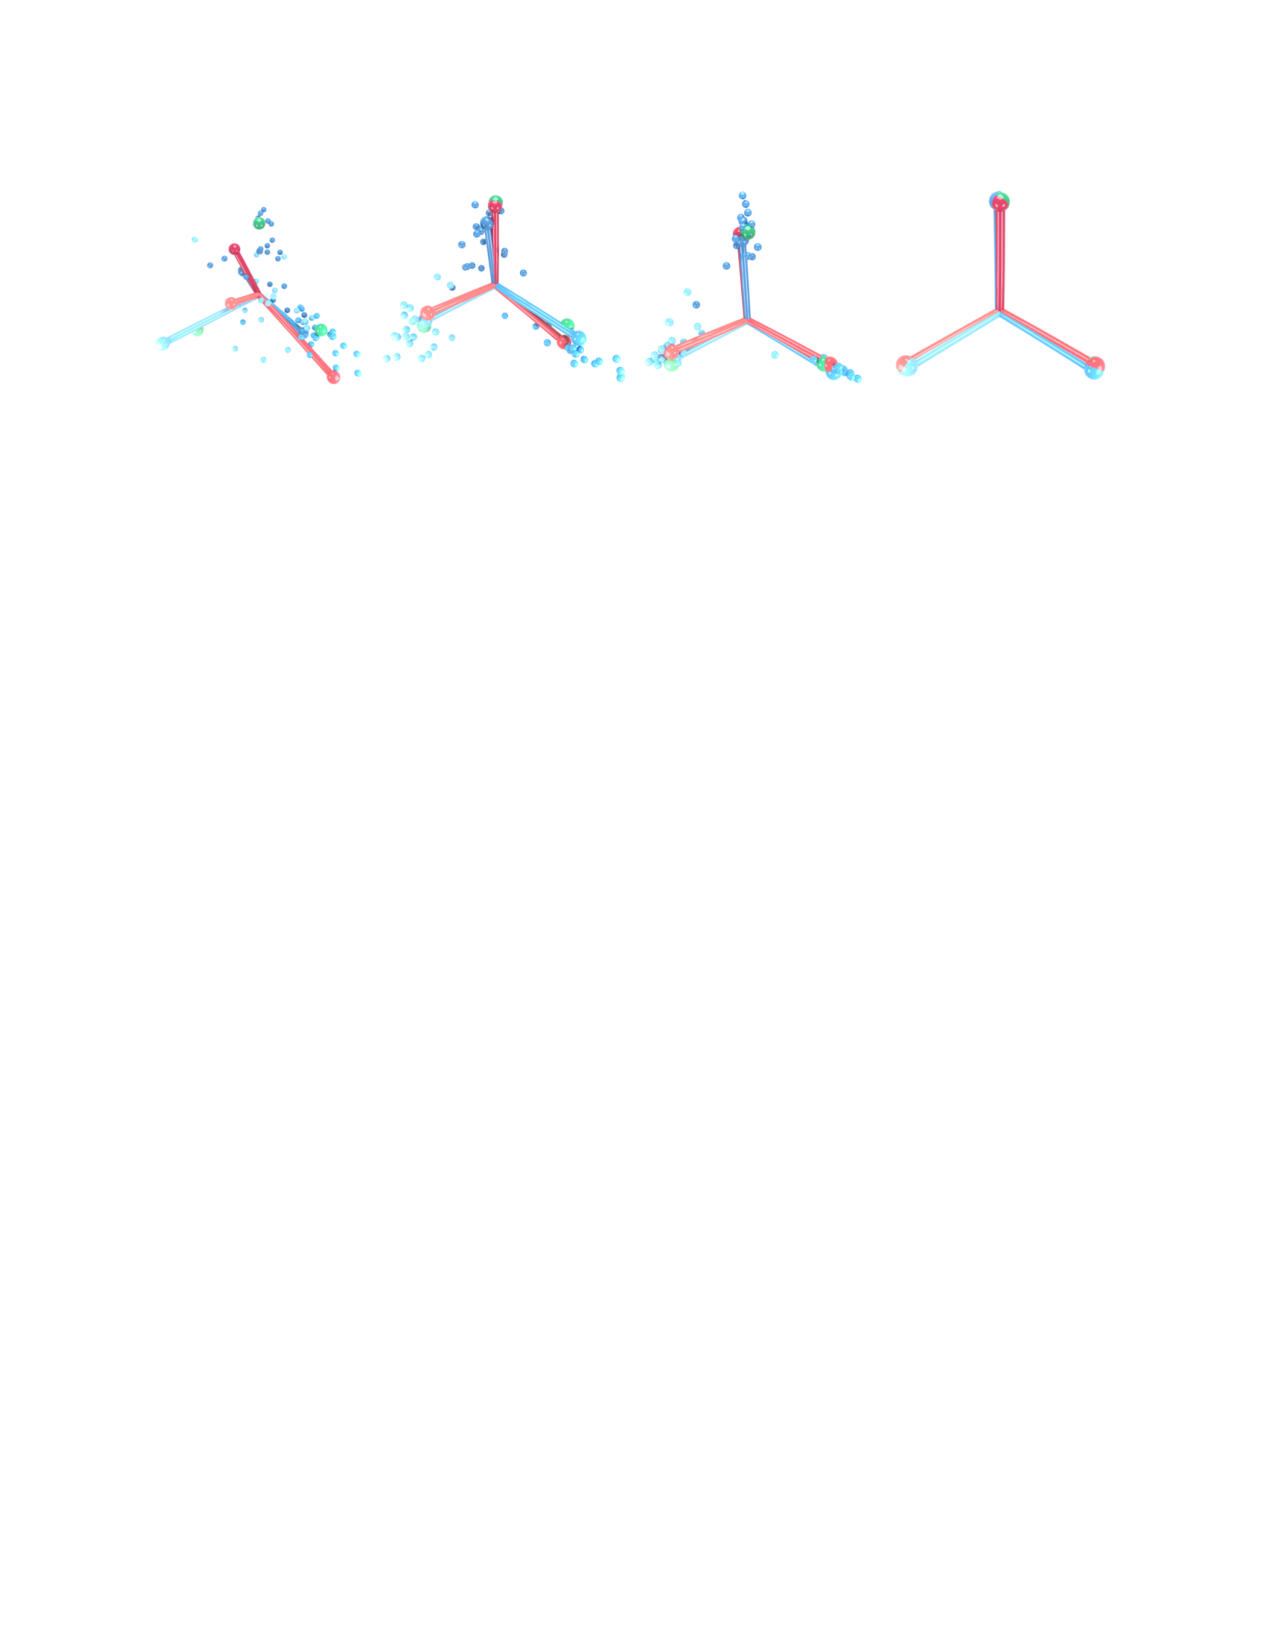
\includegraphics[width=0.95\linewidth]{\toplevelprefix/chapters/chapter3/figs/neural_collapse.pdf}
	\caption{在 CIFAR10 数据集上使用 3 个随机选择的类别训练 VGG13 神经网络时,倒数第二层输出的演变。图片来自 \cite{papyan2020prevalence}。}
	\label{chap4-fig:neural-collapse}
\end{figure}

\paragraph{通过信息瓶颈获得最小判别特征。}
一种解释深度网络作用的流行方法是将网络中间层的输出视为选择数据的某些潜在特征 $\z = f(\x, \theta) \in \Re^d$,这些特征在多个类别之间具有判别性。学习到的表示 $\z$ 然后通过优化一个分类器 $g(\z)$ 来促进后续的分类任务,以预测类别标签 $\y$:
\begin{equation}
	\x   \xrightarrow{\hspace{2mm} f(\x, \theta)\hspace{2mm}} \z  \xrightarrow{\hspace{2mm} g(\z) \hspace{2mm}} \y.
\end{equation}
我们从信息论~\cite{Cover-Thomas} 中知道,两个随机变量(比如说 $\x,\z$)之间的{\em 互信息}定义为
\begin{equation}
	I(\x; \z) = H(\x) - H(\x\mid \z),
\end{equation}
其中 $H(\x \vert \z)$ 是给定 $\z$ 时 $\x$ 的条件熵。互信息也称为{\em 信息增益}:它衡量一旦给定 $\z$,随机变量 $\x$ 的熵可以减少多少。或者等价地,它衡量 $\z$ 包含关于 $\x$ 的多少信息。{\em 信息瓶颈}(IB)公式 \cite{Tishby-ITW2015} 进一步假设网络的作用是学习 $\z$ 作为预测 $\y$ 的最小充分统计量。形式上,它寻求最大化 $\z$ 和 $\y$ 之间的互信息 $I(\z, \y)$,同时最小化 $\x$ 和 $\z$ 之间的互信息 $I(\x, \z)$:
\begin{equation}
	\max_{\theta\in \Theta}\; \mbox{IB}(\x, \y, \z) \doteq I(\z; \y) - \beta I(\x; \z) \quad\ \mathrm{s.t.}\ \z = f(\x, \theta),
	\label{chap4-eqn:information-bottleneck}
\end{equation}
其中 $\beta >0$。

如果能克服这个框架的一些注意事项 \cite{kolchinsky2018caveats-ICLR2018},例如如何用有限的退化分布样本准确评估互信息,这个框架可以帮助解释深度网络的某些行为。
例如,最近的工作 \cite{papyan2020prevalence} 确实表明,通过交叉熵损失 \eqref{chap4-eqn:cross-entropy} 学习到的表示表现出一种\emph{神经坍塌}现象。
也就是说,每个类别的特征被映射到一个一维向量,而该类别的所有其他信息都被抑制了,如图~\ref{chap4-fig:neural-collapse} 所示。
% % \footnote{Essentially, once an over-parameterized network fits the training data, regularization (such as weight decay) would collapse weight components or features that are not the most relevant for fitting the class labels. Besides the most salient feature, informative and discriminative features that also help define a class can be suppressed.} 
% where within-class variability and structural information are getting suppressed and ignored, as illustrated in Figure~\ref{chap4-fig:neural-collapse}. 
\begin{remark}
    神经坍塌是指在为分类任务训练的深度神经网络中观察到的一种现象,其中学习到的特征表示和分类器权重在训练的最后阶段表现出高度对称和结构化的行为 \cite{papyan2020prevalence,zhu2021geometric}。具体来说,在每个类别内,特征坍塌到它们的类别均值,而在类别之间,这些均值变得最大程度地分离,形成一个单纯形等角配置。线性分类器与类别均值对齐,直到重新缩放。此外,最后一层分类器收敛到选择具有最近训练类别均值的类别。神经坍塌揭示了优化动力学、泛化和监督学习中出现的几何结构之间的深层联系。
\end{remark}

从上面的分类例子中,我们看到,如此学习到的表示给出了一个非常简单的编码器,它基本上将每一类数据映射到仅一个码字:代表每个类别的独热向量。从有损压缩的角度来看,这样的编码器损失太大,无法保留数据分布中的信息。其他信息,例如对图像生成等任务有用的信息,在这样的监督学习过程中被严重丢失了。为了弥补这种情况,我们希望学习一个不同的编码方案,使得最终的特征表示能够捕捉到关于数据分布的更丰富的信息,而不仅仅是用于分类的信息。

% Here by being task-dependent (depending on the label $\y$) and seeking a {\em minimal} set of most informative features for the task at hand (for predicting the label $\y$ only), the so learned network may sacrifice robustness in case the labels can be corrupted or transferability when we want to use the features for different tasks. To address this, we

% {\em the framework -- we will present in this chapter -- uses the label $\y$ as only side information to assist learning discriminative yet diverse (not minimal) representations; these representations optimize a different intrinsic objective based on }

\begin{figure}[ht]
	\centering
	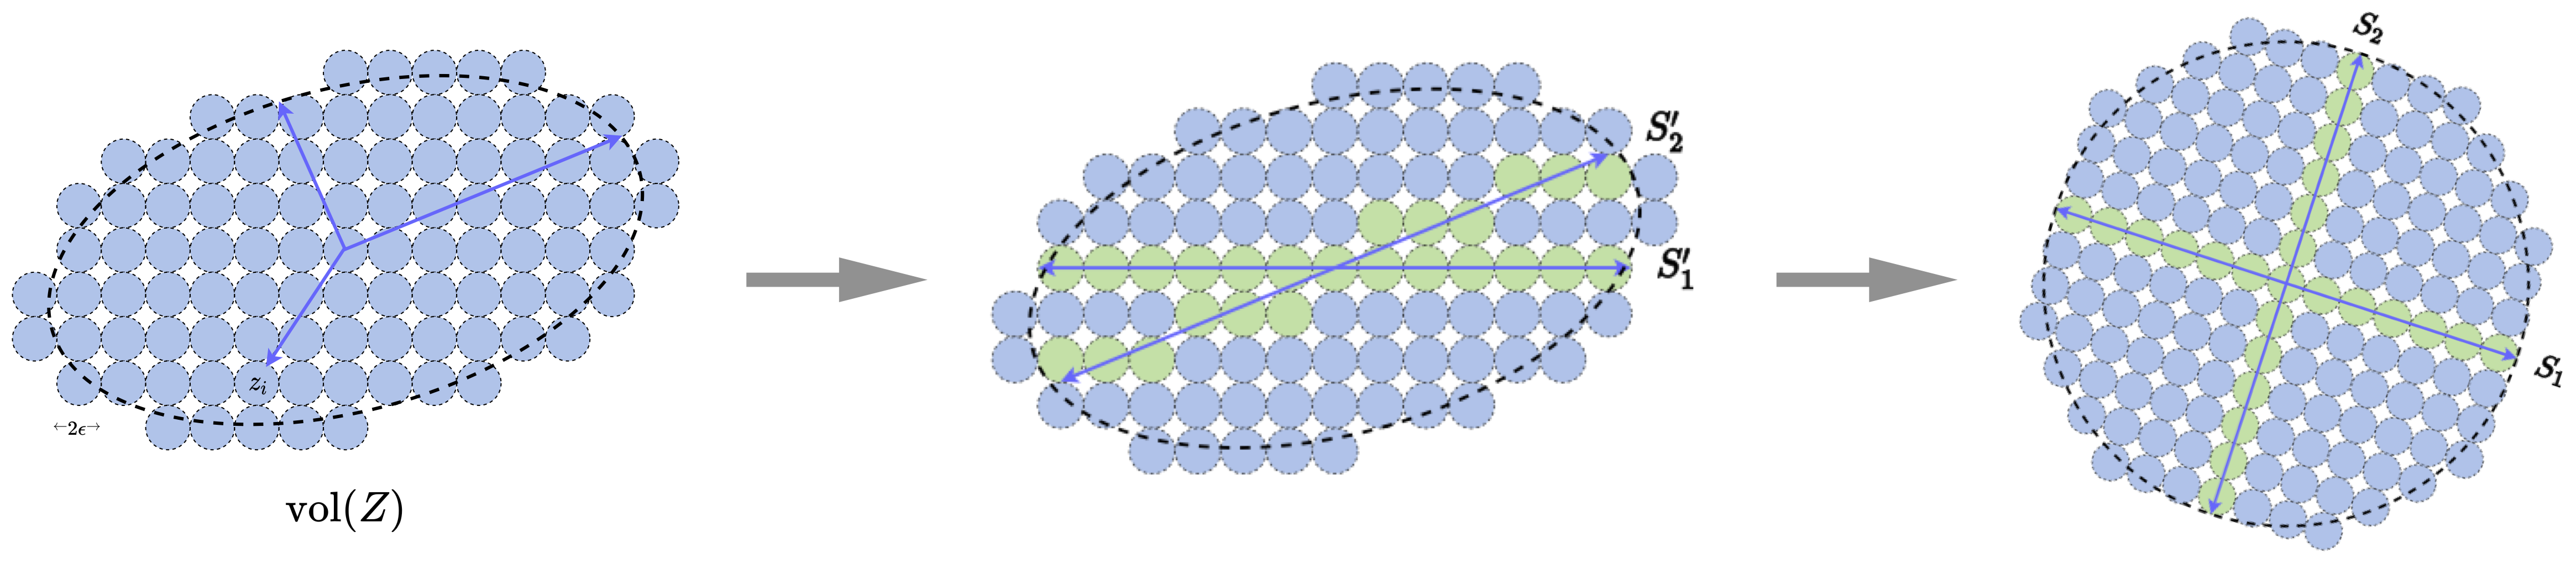
\includegraphics[width=0.99\linewidth]{\toplevelprefix/chapters/chapter3/figs/Expansion2.png}
	\caption{在识别出低维数据分布后,我们希望进一步将数据分布转换为更具信息量的结构表示:$R$ 是覆盖整个空间的 $\epsilon$-球的数量,$R^c$ 是所有子空间(绿色球)的总数。$\Delta R$ 是它们的差值(蓝色球的数量)。}\label{fig:sphere-packing}
	\label{fig:informative-representation}
\end{figure}


\paragraph{线性判别表示。}
给定的混合分布 $\mathcal{D}$ 的数据 $\X$ 是否能被有效分类或聚类,取决于成分分布 $\mathcal{D}_k$ 的可分性(或判别性)如何(或可以被塑造成如何)。一个流行的工作假设是,每个类别的分布都具有相对{\em 低维}的内在结构。因此,我们可以假设每个类别的分布 $\mathcal{D}_k$ 的支撑集位于一个低维子流形上,比如说维度为 $d_k \ll D$ 的 $\mathcal{M}_k$,而 $\x$ 的分布 $\mathcal D$ 的支撑集位于这些子流形的混合体 $\mathcal M = \cup_{k=1}^K \mathcal{M}_k$ 上,在高维环境空间 $\Re^D$ 中。

我们不仅需要识别低维分布,还希望以一种最能促进后续任务(如分类、聚类和条件生成,我们将在未来看到)的形式来表示该分布。为此,我们要求我们学习到的特征表示具有以下属性:
\begin{enumerate}
	\item {\em 类内可压缩:} 来自同一类别的样本的特征应该高度{\em 相关},即它们属于一个低维线性子空间。
	\item {\em 类间可判别:} 来自不同类别的样本的特征应该高度{\em 不相关},并属于不同的低维线性子空间。
	\item {\em 最大化多样性表示:} 每个类别的特征的维度(或方差)应该{\em 尽可能大},只要它们与其他类别不相干。
\end{enumerate}
我们将这样的表示称为{\em 线性判别表示}(LDR)。请注意,第一个属性与我们在第 \ref{sub:pca} 章中讨论的经典{\em 主成分分析}(PCA)的目标非常吻合。第二个属性类似于经典的{\em 线性判别分析}(LDA)~\cite{HastieTiFr09}。图 \ref{fig:informative-representation} 用一个简单的例子说明了这些属性,当数据分布实际上是两个子空间的混合时。通过压缩(去噪或聚类),我们首先识别出真实的数据分布是两个低维子空间的混合(中),而不是一个通用的高斯分布(左)。然后,我们希望转换分布,使两个子空间最终变得相互不相干/独立(右)。

\begin{remark}
    线性判别分析(LDA)~\cite{HastieTiFr09} 是一种监督降维技术,旨在找到数据的线性投影,以最大化类别可分性。具体来说,给定带标签的数据,LDA 寻求一个线性变换,将高维输入投影到一个低维空间,在该空间中类别被最大程度地分离。请注意,PCA 是一种无监督方法,它将数据投影到最大方差的方向,而不考虑类别标签。虽然 PCA 纯粹关注于保留全局方差结构,但 LDA 明确利用标签信息来增强判别能力;参见 \Cref{fig:LDA} 中的比较。
\end{remark}

\begin{figure}
	\centering
	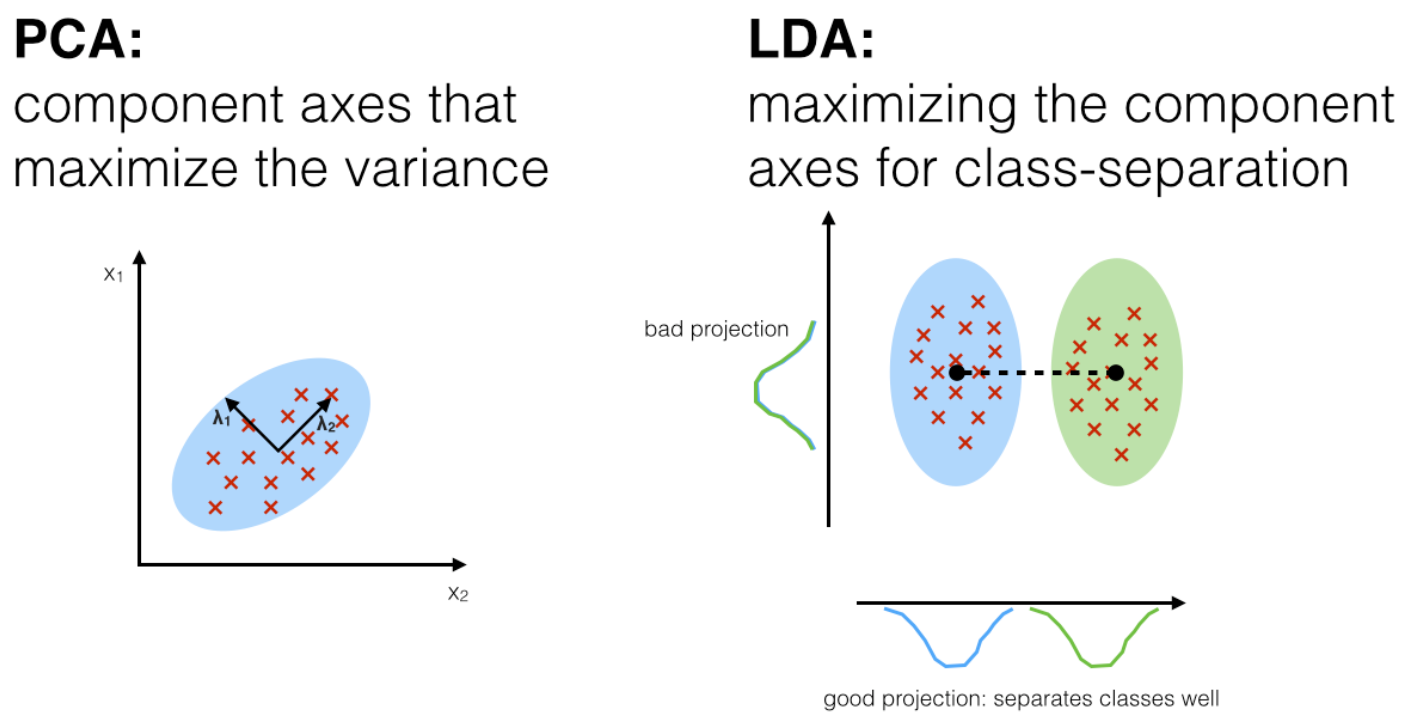
\includegraphics[width=0.7\linewidth]{\toplevelprefix/chapters/chapter3/figs/LDA.png}\vspace{-0.1in}
	\caption{PCA 和 LDA 之间的比较。图片改编自 \url{https://sebastianraschka.com/Articles/2014_python_lda.html}。}
	\label{fig:LDA}
\end{figure}


第三个属性也很重要,因为我们希望学习到的特征能揭示一个类别与所有其他类别不同的所有可能原因。例如,要区分“苹果”和“橙子”,我们不仅关心颜色,还关心形状和叶子。理想情况下,每个子空间 $\{\mathcal{S}_k\}$ 的维度应该等于相应子流形 $\mathcal{M}_k$ 的维度。如果我们希望映射 $f(\x,\theta)$ 对于图像生成等任务是{\em 可逆的},这个属性将很重要。例如,如果我们从“苹果”的特征子空间中抽取不同的样本点,我们应该能够将它们解码以生成各种各样的苹果图像。从最小化交叉熵 \eqref{chap4-eqn:cross-entropy} 中学习到的特征显然不具备这个属性。


总的来说,尽管每个类别/聚类的内在结构可能是低维的,但它们在其原始表示 $\x$ 中绝不是简单的线性(或高斯)的,它们需要首先通过一些非线性变换变得线性。\footnote{我们将在第 \ref{ch:autoencoding} 章中讨论如何明确地做到这一点。} 因此,总的来说,我们使用非线性变换 $f(\x,\theta)$ 来寻求数据的表示,使得代表所有类别的子空间是最大程度不相干的线性子空间。更准确地说,我们希望学习一个映射 {$\z = f(\x,\theta)$},它将每个子流形 $\mathcal{M}_k \subset \Re^D$(图~\ref{chap4-fig:mcr-diagram} 左)映射到一个{\em 线性}子空间 $\mathcal{S}_k \subset \Re^d$(图~\ref{chap4-fig:mcr-diagram} 右)。在某种程度上,得到的多个子空间 $\{\mathcal{S}_k\}$ 可以被看作是原始数据 $\bm x$ 的判别性{\em 广义主成分} \cite{GPCA},或者,如果是正交的,则是结果特征 $\z$ 的{\em 独立成分} \cite{hyvarinen2000independent}。
正如我们将在下一章 \ref{ch:representation} 中看到的,深度网络正是扮演着建模和实现从数据分布到线性判别表示的这种非线性变换的角色。


%\subsection{The Principle of Maximal Information Gain}
\subsection{最大编码率降低原则}\label{subsec:MCR2}



%\paragraph{Classic  Information Gain.}  The classic  {\em Information Gain} (IG), which aims to maximize the reduction of entropy of a random variable, say $\bm z$, with respect to an observed attribute, say $\bm \pi$:$\max_{\bm \pi} \; \mbox{IG}(\bm z, \bm \pi) \doteq H(\bm z) - H(\bm z \mid \bm \pi),$i.e., the {\em mutual information} between $\z$ and $\bm \pi$ \cite{Cover-Thomas}. Maximal information gain has been widely used in areas such as decision trees \cite{decision-trees}. However, MCR$^2$ is used differently in several ways: 1) A typical setting of MCR$^2$ is when the data class labels are given, i.e. $\bm \Pi$ is known, MCR$^2$ focuses on learning representations $\bm z(\theta)$ rather than fitting labels. 2) In traditional settings of IG, the number of attributes in $\bm z$ cannot be so large and their values are discrete (typically binary). Here, the ``attributes'' $\bm \Pi$  represent the probability of a multi-class partition for all samples and their values can even be continuous. 3) As mentioned before, entropy $H(\bm z)$ or mutual information $I(\bm z, \bm \pi)$ \cite{hjelm2018learning} is not well-defined for degenerate continuous distributions whereas the rate distortion $R(\bm z, \epsilon)$ is and can be accurately and efficiently computed for (mixed)  subspaces, at least.


尽管这三个属性——{\em 类间可判别}、{\em 类内可压缩}和{\em 最大化多样性表示}——对于线性判别表示(LDR)都是非常理想的属性,但它们绝不容易获得:这些属性是否兼容,以至于我们可以期望一次性实现它们?如果是这样,是否存在一个{\em 简单但有原则的}目标,可以根据所有这些属性来衡量最终表示的好坏?这些问题的关键是{找到}一个有原则的“紧凑性度量”或“信息增益”,用于随机变量 $\z$ 的分布或其有限样本 $\{\bm z_i\}_{i=1}^N$。这样的度量应该直接准确地刻画分布的内在几何或统计特性,就其内在维度或{体积}而言。与交叉熵 \eqref{chap4-eqn:cross-entropy} 或信息瓶颈 \eqref{chap4-eqn:information-bottleneck} 不同,这样的度量不应完全依赖于类别标签,以便它可以在更一般的设置中工作,如监督、自监督、半监督和无监督设置。

\begin{figure}
	\centering
	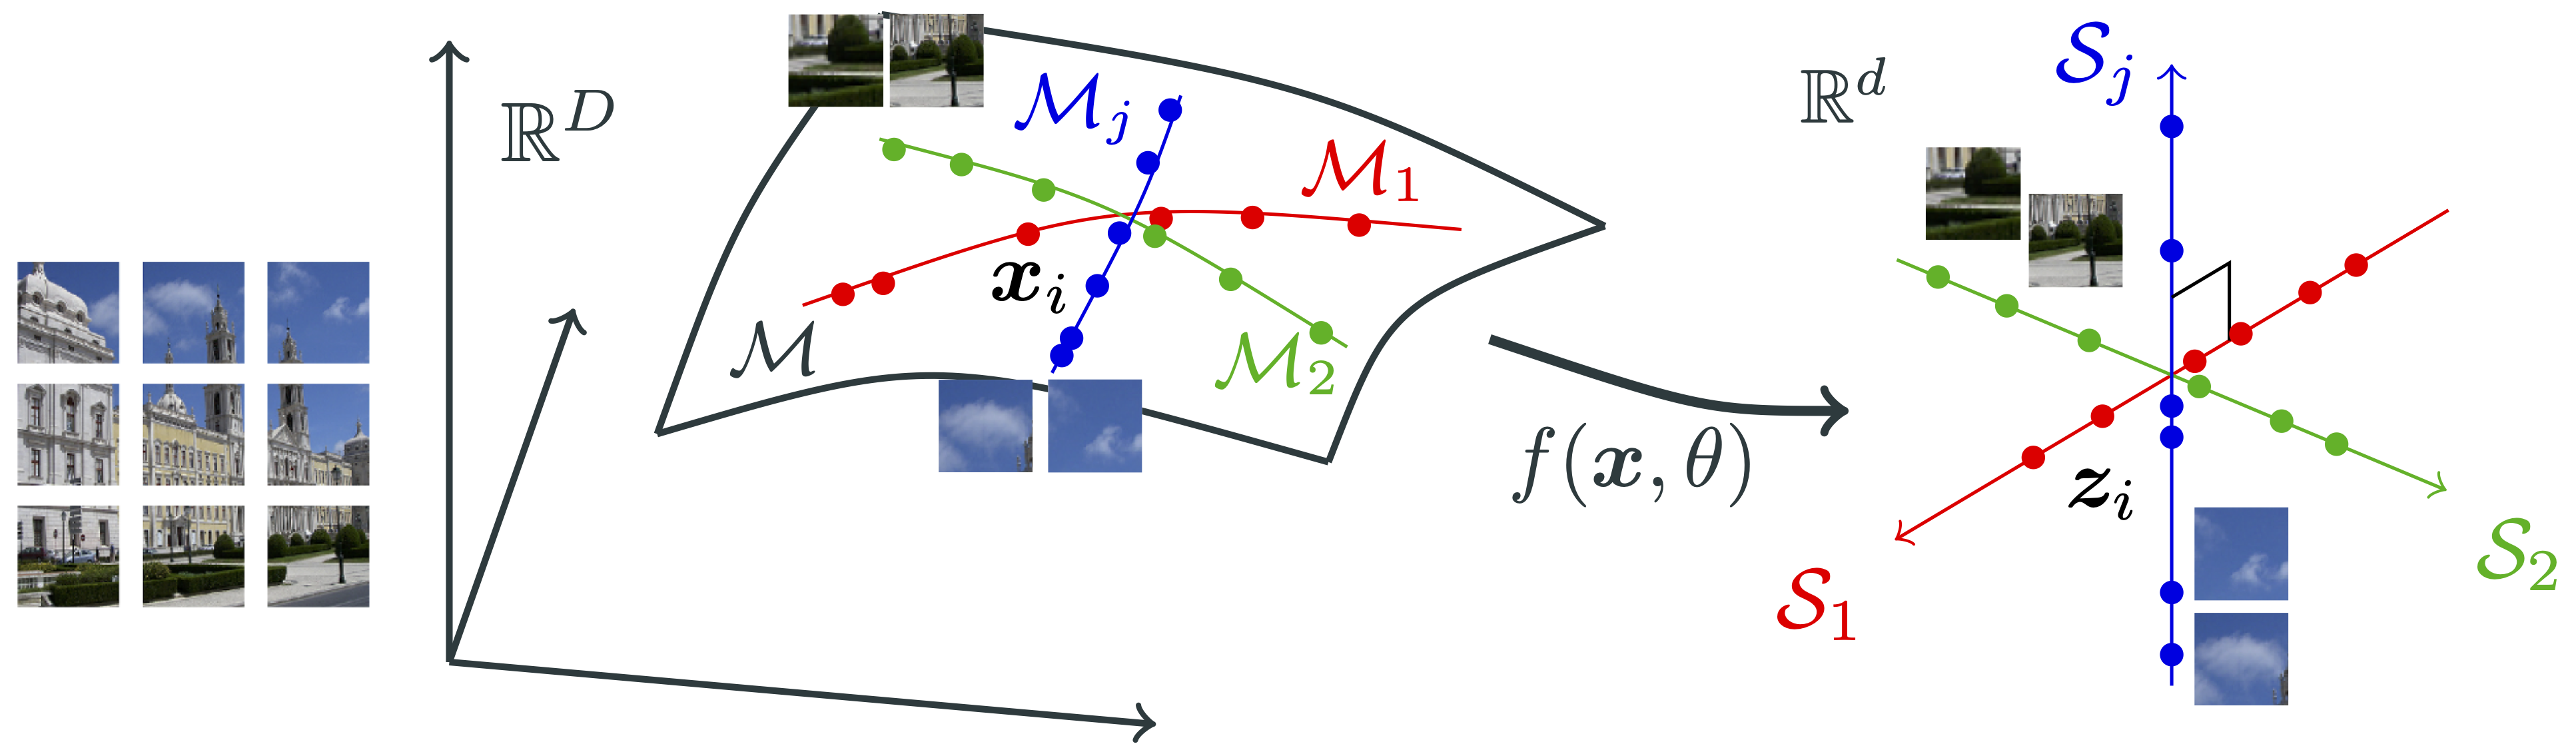
\includegraphics[width=0.8\linewidth]{\toplevelprefix/chapters/chapter3/figs/mcr_diagram.png}
	\caption{高维数据 $\x\in \Re^D$ 的分布 $\mathcal D$ 支持在一个流形 $\mathcal{M}$ 上,其类别支持在低维子流形 $\mathcal{M}_k$ 上。我们的目标是学习一个由 $\theta$ 参数化的映射 $f(\x, \theta)$,使得 $\z_i = f(\x_i, \theta)$ 位于最大程度不相关的子空间 $\{\mathcal{S}_k\}$ 的并集上。}
	\label{chap4-fig:mcr-diagram}
\end{figure}
% As we discussed above, we would like the learned representation to preserve as much information about $\x$. If so, one can approximately recover $\x$ from the corresponding $\z$. In other words, there exists a decoding map $g(\z)$ such that
% \begin{equation}
%     \x   \xrightarrow{\hspace{2mm} f(\x)\hspace{2mm}} \z  \xrightarrow{\hspace{2mm} g(\z) \hspace{2mm}} \hat{\x},
% \end{equation}
% where $\hat{\x}$ closely approximates $\x$. Hence we would like to maximize the mutual information between $\x$ and $\hat \x$ while we want $\z$ to be as compact as possible. A natural measure of compactness for $\z$ is its entropy $H(\z)$. We want it to be minimized. Therefore, we could argue that to seek a good representation, we would like to maximize the following objective:
% \begin{equation}
%     \max I(\x, \hat{\x}) - \alpha H(\z).
%     \label{eqn:info-gain-obj1}
% \end{equation}
% Notice that $I(\x, \hat{\x}) \ge R(\hat \x,\epsilon)$ if the decoded $\hat \x$ satisfies $\mathbb E[\|\x - \hat \x \|_2] \le \epsilon$. Hence the above objective can be replaced as
% \begin{equation}
%     \max R(\hat \x,\epsilon) - \alpha H(\z).
%     \label{eqn:info-gain-obj2}
% \end{equation}

% However, differential entropy $H(\z)$ is not well-defined for continuous random variables with degenerate distributions.  This is unfortunately the case here for $\z$. In this case, strictly speaking $H(\z)$ can be negative infinity, as we can see from the differential entropy of a (nearly degenerate) Gaussian distribution in \eqref{eqn:entropy-Gaussian-multi}. To alleviate this difficulty, as we have discussed earlier in this chapter, we may use another measure of ``compactness'' of a distribution, the {\em rate distortion}: Recall that, given a random variable $\z$ and a prescribed precision $\epsilon >0$, the rate distortion $R(\z, \epsilon)$ is the minimal number of binary bits needed to encode $\z$ such that the expected decoding error is less than $\epsilon$, i.e., the decoded $\hat \z$ satisfies $\mathbb E[\|\z - \hat \z \|_2] \le \epsilon$. Hence the above objective \eqref{eqn:info-gain-obj2} can be replaced as:
% \begin{equation}
%     \max R(\hat \x,\epsilon) - \alpha R(\z, \epsilon).
%     \label{eqn:info-gain-obj3}
% \end{equation}




%To learn a discriminative linear representation for intrinsic low-dimensional structures from high-dimensional data, we here propose an information-theoretic measure that maximizes the coding rate difference between the whole dataset and the sum of each individual class, known as {\em rate reduction}. This new objective provides a more unifying view of the above objectives such as cross-entropy, information bottleneck, and contractive and contrastive learning. {\em We will rigorously show that when the intrinsic dimensions of the submanifolds are known and this objective is optimized, the resulting representation indeed has the desired properties listed above.}


% However, entropy is not well-defined for continuous random variables with degenerate distributions. The same difficulty resides with evaluating mutual information $I(\x, \z)$ for degenerate distributions.
% This is unfortunately the case here.
% To alleviate this difficulty, as we have discussed earlier in this chapter, we may use another measure of ``compactness'' of a distribution, the {\em rate distortion}:
% Given a random variable $\z$ and a prescribed precision $\epsilon >0$, the rate distortion $R(\z, \epsilon)$ is the minimal number of binary bits needed to encode $\z$ such that the expected decoding error is less than $\epsilon$, i.e., the decoded $\hat \z$ satisfies $\mathbb E[\|\z - \hat \z \|_2] \le \epsilon$.

%\yaodong{TODO: change the notion for $i$-th sample from $\bm{z}_{i}$ to $\bm{z}^{i}$, since $\bm{z}_{\ell}^{i}$ denotes the $i$-th sample at the $\ell$-th layer.}

不失一般性,假设随机向量 $\x$ 的分布 $\mathcal D$ 支持在一个分布的混合体上,即 $\mathcal D = \cup_{k=1}^K \mathcal{D}_k$,其中每个 $\mathcal{D}_k \subset \Re^D$ 在高维环境空间 $\Re^D$ 中具有低的内在维度。让 $\bm X_k \in \Re^{D\times N_k}$ 表示数据矩阵,其列是从分布 $\mathcal{D}_k$ 中抽取的样本,其中 $N_k$ 表示每个 $k=1,\dots,K$ 的样本数。然后,我们用 $\bm X=[\bm X_1,\dots,\bm X_K] \in \Re^{D\times N}$ 来表示所有样本,其中 $N=\sum_{k=1}^K N_k$。
%Suppose that we have a set of samples $\X = \cup_{j=1}^k \X_j$ drawn from the distribution $\mathcal D$, where $\X_j$ contains samples drawn from the corresponding distribution $\mathcal{D}_j$ for each $j=1,\dots,k$. 
回想一下,我们也用 $\vx_i$ 来表示 $\X$ 的第 $i$ 个样本,即 $\X=[\vx_1,\dots,\vx_N]$。在一个编码映射下:
\begin{equation}
	\x   \xrightarrow{\hspace{2mm} f(\x)\hspace{2mm}} \z,
\end{equation}
输入样本被映射到 $\vz_i = f(\vx_i)$,对于每个 $i=1,\dots,N$。滥用符号,我们也写 $\Z_k = f(\X_k)$ 和 $\Z = f(\X)$。因此,我们有 $\Z = [\bm Z_1,\dots,\bm Z_K]$ 和 $\Z = [\vz_1,\dots\vz_N]$。

一方面,为了使学习到的特征具有判别性,不同类别/聚类的特征最好是{\em 最大程度不相关的}。因此,它们一起应该张成一个尽可能大体积(或维度)的空间,并且整个集合 $\Z$ 的编码率应该尽可能大。另一方面,同一类别/聚类的学习到的特征应该高度相关和一致。因此,每个类别/聚类应该只张成一个非常小体积(或子空间)的空间,并且编码率应该尽可能小。现在,我们将介绍如何衡量学习到的特征的编码率。

\paragraph{特征的编码率。} 值得注意的是,评估编码率的一个实际挑战是,特征表示 $\Z$ 的底层分布通常是未知的。为了解决这个问题,我们可以将特征 $\Z = [\z_1, \ldots, \z_N]$ 近似为从一个多元高斯分布中抽取的样本。在这个假设下,正如在第 \ref{subsec:lossy DR} 章中讨论的,特征 $\Z$ {\em 作为一个整体}的紧凑性可以用每个样本的平均编码长度来衡量,称为{\em 编码率},受精度水平 $\epsilon > 0$ 的限制(见 \eqref{eqn:rate-Gaussian}),定义如下:
\begin{equation}
	R_{\epsilon}(\Z) = \frac{1}{2}\log\det\left(\I + \frac{d}{N\epsilon^{2}}\Z\Z^{\top}\right).
	\label{chap4-eqn:coding-length-eval}
\end{equation}

另一方面,我们希望一个非线性变换 $f(\x)$ 将每个特定于类别的子流形 $\mathcal{M}_k \subset \mathbb{R}^D$ 映射到一个最大程度不相关的线性子空间 $\mathcal{S}_k \subset \mathbb{R}^d$,使得学习到的特征 $\Z$ 位于低维子空间的并集上。这种结构允许通过分别分析每个子空间来更准确地评估编码率。% To this end, we partition the data $\Z$ into multiple subsets: $\Z = \Z_1 \cup \cdots \cup \Z_k$, where each subset $\Z_j$ lies within in one low-dimensional subspace. 
% The above coding rate \eqref{chap4-eqn:coding-length-eval} can then be accurately computed for each subset as follows:
% \begin{align}
%     R_{\epsilon}(\Z_j) = \frac{1}{2} \log\det\left(\I + \frac{d}{N_j\epsilon^{2}}\Z_j\Z_j^{\top}\right),
% \end{align}
% where $N_j$ denotes the number of samples in $\Z_j$. 
% For convenience, let $\bm{\Pi} = \{\bm{\Pi}^j \in \Re^{N \times N}\}_{j=1}^{k}$ be a set of diagonal matrices whose diagonal entries encode the membership of the $N$ samples in the $k$ classes. More specifically, the diagonal entry $\bm \Pi^j(i,i)$ of $\bm \Pi^j$ indicates the probability of sample $i$ belonging to subset $j$. Therefore $\bm{\Pi}$ lies in a simplex: ${\Omega} \doteq \{\bm{\Pi} \mid \bm{\Pi}^j \ge \mathbf{0}, \; \bm{\Pi}^1 + \cdots + \bm{\Pi}^k = \I\}$. 
回想一下,$\Z_k$ 的列表示 $\X_k$ 中样本的特征,对于每个 $k=1,\dots,K$。$\bm Z_k$ 中特征的编码率可以计算如下:
\begin{align}
    R_{\epsilon}(\Z_k) = \frac{N_k}{2N}\log\det\left(\I + \frac{d}{N_k\epsilon^{2}}\Z_k\Z_k^{\top}\right)
\end{align}
那么,每个类别中特征的平均编码率之和是
\begin{equation}
	 R_{\epsilon}^c(\Z) \doteq \sum_{k=1}^K R_{\epsilon}(\Z_k),
	\label{chap4-eqn:compress-loss-eval}
\end{equation}
% Note that when $\Z$ is given, $R_{\epsilon}^c(\Z \mid \bm{\Pi})$ is a concave function of $\bm{\Pi}$.
% The function $\log\det(\cdot)$ in the above expressions has been long known as an effective heuristic for rank minimization problems, with guaranteed convergence to local minimum \cite{fazel2003log-det}. {As it nicely characterizes the coding rate of Gaussian or subspace-like distributions, $\log\det(\cdot)$ can be very effective in clustering or classification of data that are mixed Gaussians \cite{ma2007segmentation}.} Note that for the clustering purpose alone, one may only care about the sign of $\Delta R$ to decide whether to partition the data or not, which leads to the greedy clustering Algorithm \ref{alg:steepest_descent_coding_length} studied in the previous section. More specifically, in the context of clustering {\em finite} samples, one needs to use the more precise measure of the coding length mentioned earlier in Section \ref{sec:clustering-Gaussians}. See \cite{ma2007segmentation} for more details.
% As discussed in Chapter \ref{subsec:lossy DR}, we can use the metric  \eqref{eq:coding rate} to measure the compactness (i.e., coding rate) for the whole set of the features and want $R_{\epsilon}(\bm Z)$ to be large. 
% Hence we want the coding rate (or length) for the whole set of features $R_{\epsilon}(\Z)$ to be large (see \eqref{chap4-eqn:coding-length-eval}). \pw{We should relate here to Chpa 3.3.3!} 
% Hence we want the coding rate for each subset $\Z_j$ to be small. We denote the sum of all these coding rates as
 % where $\bm \Pi$ denotes the partition $\Z \rightarrow \cup_{j=1}^k \Z_j$.

因此,一个好的 $\X$ 的表示 $\Z$ 是那个能够实现整个编码率与所有类别编码率之和之间最大差异的表示:
\begin{equation}
	\Delta R_{\epsilon}(\Z) \doteq R_{\epsilon}(\Z) - R_{\epsilon}^c(\Z).
	\label{chap4-eqn:coding-length-reduction}
\end{equation}
请注意,根据我们本章早些时候的讨论,这个差异可以被解释为通过识别总体集合 $\Z$ 内正确的低维聚类 $\Z_k$ 而“获得的信息”量。

如果我们将特征映射 $f(\cdot)$ 选择为一个具有网络参数 $\theta$ 的深度神经网络 $f(\cdot,\theta)$,那么特征表示的整个过程以及由此产生的率降低可以通过以下图示来说明:
\begin{equation}
	\X
	\xrightarrow{\hspace{2mm} f(\x, \theta)\hspace{2mm}} \Z  \xrightarrow{\hspace{2mm} \epsilon \hspace{2mm}} \Delta R_{\epsilon}(\Z).
	\label{chap4-eqn:flow}
\end{equation}
请注意,$\Delta R_{\epsilon}$ 在特征 $\Z$ 的尺度上是{\em 单调的}。为了确保不同表示之间的公平比较,对学习到的特征的尺度进行{\em 归一化}至关重要。这可以通过对每个类别 $\Z_k$ 的弗罗贝尼乌斯范数施加与 $\Z_k \in \mathbb R^{d \times N_k}$ 中特征数量成比例的约束,即 $\|\Z_k\|_F^2 = N_k$,或者通过将每个特征归一化到单位球面上,即 $\z_i \in \mathbb{S}^{d-1}$ 来实现,其中 $N_k=\mathrm{tr}(\bm \Pi_k)$ 表示第 $k$ 类中的样本数量。这个公式为在训练深度神经网络的实践中需要“批量归一化”提供了自然的理由 \cite{ioffe2015batch}。% An alternative, arguably simpler, way to normalize the scale of learned representations is to ensure that the mapping of each layer of the network is approximately {\em isometric} \cite{ISOnet}.

一旦表示是可比较的,目标就变成了学习一组特征 $\Z = f(\X, \theta)$,使得它们最大化所有特征的编码率与各类别特征之和的编码率之间的降低:
\begin{equation}
	\begin{aligned}
		\max_{\theta } & \;  \Delta R_{\epsilon}\big(\Z \big) \doteq R_{\epsilon}(\Z) - R_{\epsilon}^c(\Z ), \\
		\mbox{s.t.} & \ \ \, \Z = f(\bm X, \theta),\  \|\Z_k\|_F^2                                          = N_k,\ k=1,\dots,K. 
	\end{aligned}
	\label{eqn:maximal-rate-reduction}
\end{equation}
我们称之为{\em 最大编码率降低}(MCR$^2$)原则,这是亚里士多德名言的真实体现:
\begin{quote}
	\centering
	“{\em 整体大于部分之和。}”
\end{quote}
为了学习最好的表示,我们要求{\em 整体最大程度地大于其各部分之和}。让我们再次审视图 \ref{fig:informative-representation} 中所示的例子。从压缩的角度来看,右侧的表示是{\em 最紧凑的},因为当所有特征被编码为单个高斯分布(蓝色)时的编码率与当特征被正确聚类并编码为两个独立的子空间(绿色)时的编码率之间的差异是最大的。\footnote{直观地说,由所有特征张成的整个空间的“体积”与特征实际占据的体积之间的比率是最大的。}

 
    请注意,上述 MCR$^2$ 原则是为监督学习问题设计的,其中组成员关系(或类别标签)是已知的。然而,这个原则可以自然地扩展到无监督学习问题,通过引入一个成员关系矩阵,该矩阵编码了每个数据点到潜在组或聚类的(可能是软的)分配。具体来说,设 $\bm \Pi = \{\bm \Pi_k\}_{k=1}^K \subset \R^{N\times N}$ 是一组对角矩阵,其对角线元素编码了 $N$ 个样本到 $K$ 个类别的成员关系。也就是说,$\bm \Pi$ 位于一个单纯形 $\Omega \doteq \{\bm \Pi: \bm \Pi_k \ge \bm 0: \sum_{k=1}^K \bm \Pi_k = \bm I_N\}$ 中。然后,我们可以定义关于划分 $\bm \Pi$ 的平均编码率为
    \begin{align}\label{eq:MCRc}
        R_{\epsilon}^c(\Z \mid \bm \Pi) \doteq \sum_{k=1}^K \frac{\mathrm{tr}(\bm \Pi_k)}{2N}\log\det\left(\bm I + \frac{d}{\mathrm{tr}(\bm \Pi_k)\epsilon^2}\bm Z\bm \Pi_k \bm Z^\top \right).
    \end{align}
    当 $\bm Z$ 给定时,$R_{\epsilon}^c(\Z \vert \bm \Pi)$ 是 $\bm \Pi$ 的一个凹函数。那么,无监督学习问题的 MCR$^2$ 原则变为如下:
    \begin{align}\label{eq:MCR pi}
        \max_{\bm \Pi, \theta} & \  \Delta R_{\epsilon}\big(\Z  \mid \bm \Pi) \doteq R_{\epsilon}(\bm Z) - R_{\epsilon}^c(\Z \mid \bm \Pi) \notag \\ 
       \mathrm{s.t.}  & \ \ \ \bm Z = f(\bm X, \theta),\ \|\bm Z \bm \Pi_k\|_F^2 = N_k,\ k = 1,\dots,K,\ \bm\Pi \in \Omega. 
    \end{align}
    与 \eqref{eqn:maximal-rate-reduction} 相比,这里的公式允许对组成员关系和网络参数进行联合优化。特别是,当 $\bm \Pi$ 固定为一个将 $N$ 个数据点分配到 $K$ 个组的组成员关系矩阵时,问题 \eqref{eq:MCR pi} 可以恢复问题 \eqref{eqn:maximal-rate-reduction}。
 


% \paragraph{Relationship to Classic  Information Gain.}
%  The maximal coding rate reduction can be viewed as a generalization to the classic  {\em Information Gain} (IG), which aims to maximize the reduction of entropy of a random variable, say $\bm z$, with respect to an observed attribute, say $\bm \pi$:
% $
% \max_{\bm \pi} \; \mbox{IG}(\bm z, \bm \pi) \doteq H(\bm z) - H(\bm z \mid \bm \pi),
% $
% i.e., the {\em mutual information} between $\z$ and $\bm \pi$ \cite{Cover-Thomas}. Maximal information gain has been widely used in areas such as decision trees \cite{decision-trees}.
% However, MCR$^2$ is used differently in several ways: 1) A typical setting of MCR$^2$ is when the data class labels are given, i.e. $\bm \Pi$ is known, MCR$^2$ focuses on learning representations $\bm z(\theta)$ rather than fitting labels. 2) In traditional settings of IG, the number of attributes in $\bm z$ cannot be so large and their values are discrete (typically binary).
% Here, the ``attributes'' $\bm \Pi$  represent the probability of a multi-class partition for all samples and their values can even be continuous. 3) As mentioned before, entropy $H(\bm z)$ or mutual information $I(\bm z, \bm \pi)$ \cite{hjelm2018learning} is not well-defined for degenerate continuous distributions whereas the rate distortion $R(\bm z, \epsilon)$ is and can be accurately and efficiently computed for (mixed)  subspaces, at least.


% \footnote{Strictly speaking, in the context of clustering {\em finite} samples, one needs to use the more precise measure of the coding length mentioned earlier, see \cite{ma2007segmentation} for more details.}
%\cs{I believe this sentence is not strict. In greedy algorithm, we use a difference between the loss encoding before and after merge. But the difference is not \eqref{eqn:maximal-rate-reduction}. In fact, in the clustering context, the first term $R(\Z(\theta), \epsilon)$ in  \eqref{eqn:maximal-rate-reduction} is a constant.}


\begin{figure}[t]
	\centering
	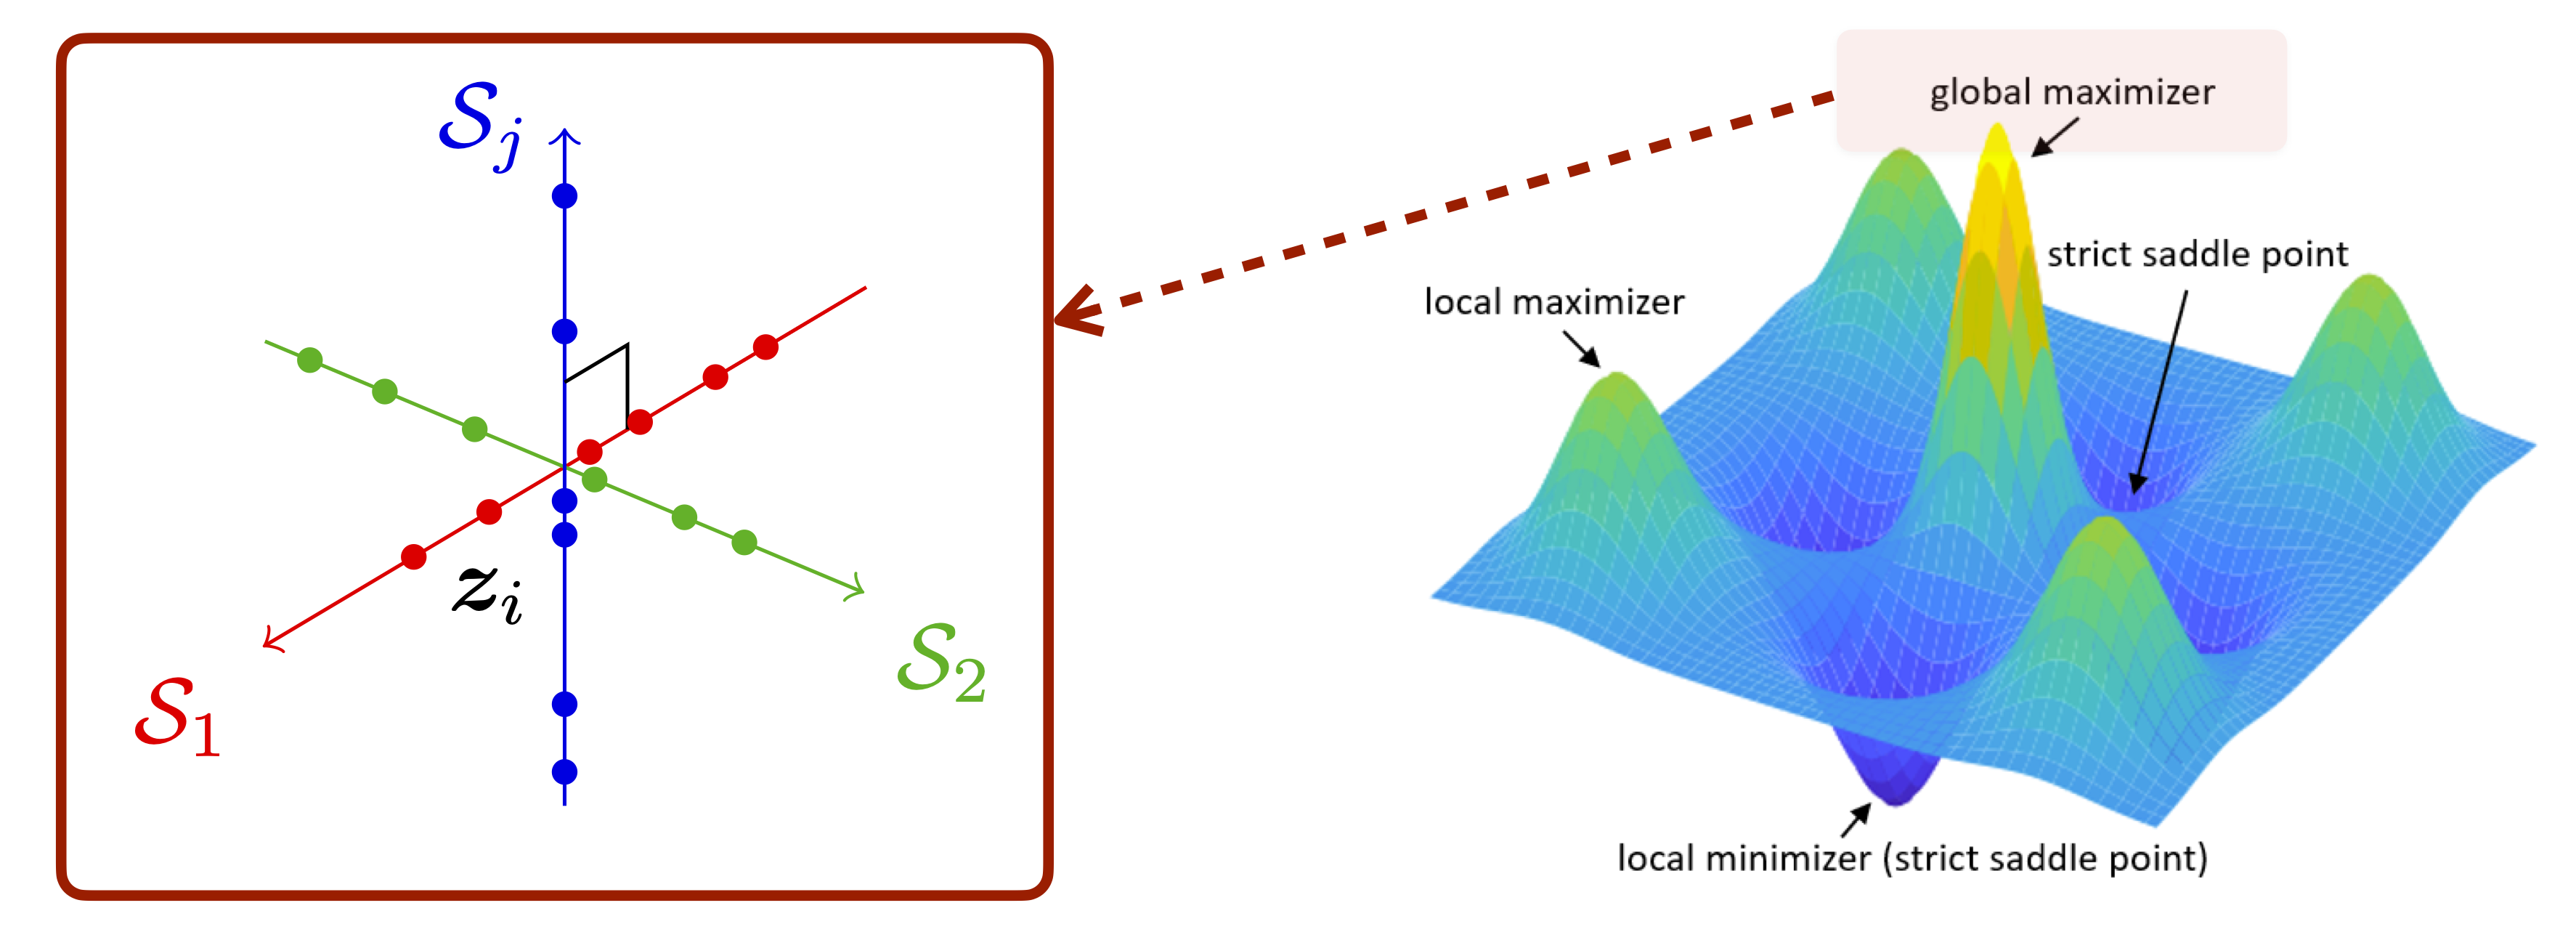
\includegraphics[width=0.8\linewidth]{\toplevelprefix/chapters/chapter3/figs/mcr2-global.png}
	\caption{{\bf 局部优化景观:} 根据定理 \ref{thm:MCR2-properties},率降低目标的全局最大值对应于一个具有相互不相干子空间的解。}
	\label{fig:mcr-global}
\end{figure}




% %\begin{wrapfigure}{r}{0.5\textwidth}
% \begin{figure}
% \begin{center}
% % \vskip -0.3in
% \includegraphics[width=0.65\textwidth]{figures_compress/pack_CompressPdf.pdf}
% \end{center}
% \vskip -0.05in
% \caption{\small Comparison of two learned representations $\Z$ and $\Z'$ via reduced rates: $R$ is the number of $\epsilon$-balls packed in the joint distribution and $R^c$ is the sum of the numbers for all the subspaces (the green balls). $\Delta R$ is their difference (the number of blue balls). The MCR$^2$ principle prefers $\Z$ (the left one).}\label{fig:sphere-packing}
% \vskip -0.15in
% \end{figure}
% %\end{wrapfigure}

% \begin{wrapfigure}{r}{0.5\textwidth}
% \vspace{-10mm}
%   \begin{center}
%     \includegraphics[width=0.47\textwidth]{figures_compress/pack_CompressPdf.pdf}%\vspace{-5mm}
%   \end{center}
%   %\addtocounter{figure}{1}
% \caption{\small Comparison of two learned representations $\Z$ and $\Z'$ via reduced rates: $R$ is the number of $\epsilon$-balls packed in the joint distribution and $R^c$ is the sum of the numbers for all the subspaces (the green balls). $\Delta R$ is their difference (the number of blue balls). The MCR$^2$ principle prefers $\Z$ (the left one).}\label{fig:sphere-packing}
% \end{wrapfigure}

\vspace{-0.1in}


\subsection{编码率降低的优化性质}
\label{sec:MCR-landscape}
% {\color{red}Geometric properties of the global optimization landscape of the rate reduction objective. MAE paper theorem that connects maximizing rate distortion to Gaussian score.}

在本小节中,我们通过分析 MCR$^2$ 函数的最优解及其优化景观的结构来研究其优化性质。为了绕过神经网络引入的技术难题,我们考虑问题 \eqref{eqn:maximal-rate-reduction} 的一个简化版本,如下所示:
\begin{align}\label{eqn1:maximal-rate-reduction}
    \max_{\bm Z}\ R_{\epsilon}(\Z) - R_{\epsilon}^c(\Z)\qquad \mathrm{s.t.}\quad \|\bm Z_k\|_F^2 = N_k,\ k =1,\dots,K. 
\end{align}
理论上,MCR$^2$ 原则 \eqref{eqn1:maximal-rate-reduction} 受益于良好的泛化性,并且可以应用于{\em 任何}分布的表示 $\Z$,只要这些分布的率 $R_\epsilon$ 和 $R^c_\epsilon$ 能够被准确高效地评估。最优表示 $\Z^{\ast}$ 应该具有一些有趣的几何和统计性质。我们在这里揭示了最优表示在子空间的特殊情况下的良好性质,这在机器学习中有许多重要的用例。当 $\Z$ 的期望表示是多个子空间时,\eqref{eqn1:maximal-rate-reduction} 中的率 $R_\epsilon$ 和 $R^c_\epsilon$ 分别由 \eqref{chap4-eqn:coding-length-eval} 和 \eqref{chap4-eqn:compress-loss-eval} 给出。在最大率降低时,MCR$^2$ 达到其最优表示,记作 $\Z^{\ast} = [\Z_1^*,\dots,\Z_K^*]$,其中 $\rank{(\Z_{k}^*)}\le d_k$。可以证明 $\Z^{\ast}$ 具有以下期望的性质(参见 \cite{yu2020learning} 获取正式陈述和详细证明)。

\begin{theorem}[\bf 全局最优解的刻画]
	假设 $\Z^{\ast} = [\Z_1^*,\dots,\Z_K^*]$ 是问题~\eqref{eqn1:maximal-rate-reduction} 的一个全局最优解。以下陈述成立:
	\begin{itemize}
		\item {\em 类间可判别}:只要环境空间足够大($d \ge \sum_{k=1}^{K} d_k$),子空间就都是相互正交的,{\em 即},对于 $k \not= l$,有 $(\Z_{k}^*)^{\top} \Z_{l}^* = \bm{0}$。
		\item {\em 最大化多样性表示}:只要编码精度足够高,即 $\epsilon ^4 < c\cdot \min_{k}\left\{ \frac{N_k}{N}\frac{d^2}{d_k^2}\right\}$,其中 $c>0$ 是一个常数。每个子空间都达到其最大维度,即 $\mathrm{rank}{(\Z_{k}^*)}= d_k$。此外,$\Z_{k}^*$ 的最大的 $d_k-1$ 个奇异值是相等的。
		      \label{thm:MCR2-properties}
	\end{itemize}
	% \vspace{-2mm}
\end{theorem}

% \begin{figure}[t]
% % \vspace{-5mm}
%     % 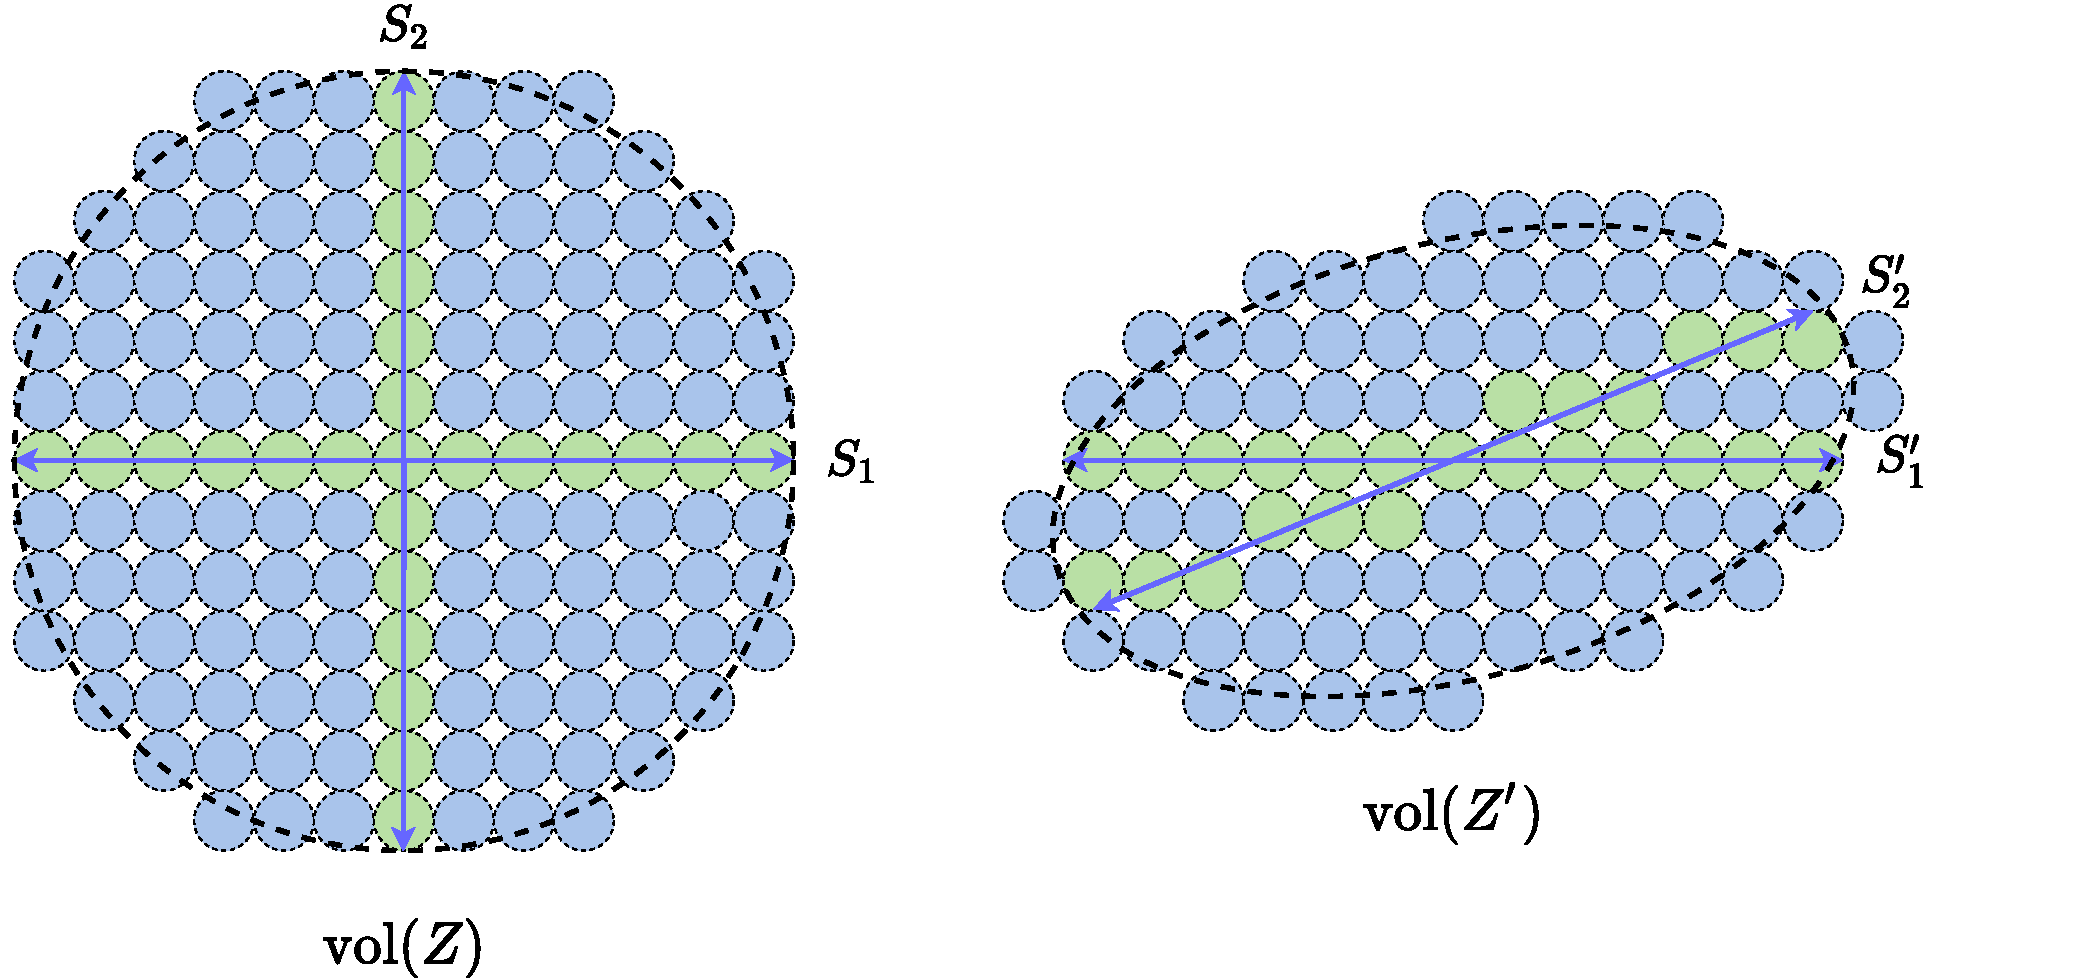
\includegraphics[width=0.7\textwidth]{chapters/chapter3/figs/pack_Compress.pdf}
% % \vspace{-15mm}
% \caption{\small Comparison of two learned representations $\Z$ and $\Z'$ via reduced rates: $R$ is the number of $\epsilon$-balls packed in the joint distribution and $R^c$ is the sum of the numbers for all the subspaces (the green balls). $\Delta R$ is their difference (the number of blue balls). The MCR$^2$ principle prefers $\Z$ (the left one).}\label{fig:sphere-packing}
% \vspace{-3mm}
% \end{figure}

这个定理表明,MCR$^2$ 原则促进了数据嵌入到多个独立的子空间中(如图 \ref{fig:mcr-global} 所示),并且特征在每个子空间中是{\em 各向同性}分布的(除了可能的一个维度)。值得注意的是,这个定理也证实了由 MCR$^2$ 原则学习到的特征表现出在 \Cref{subsec:LDR} 中讨论的期望的低维判别性质。此外,在所有这样的判别表示中,它偏好在环境空间中具有最高维度的那个。这与信息瓶颈的目标~\eqref{chap4-eqn:information-bottleneck} 有本质的不同。
% \pw{add some transition here to connect MCR$^2$ to the regularized MCR$^2$}\yaodong{TODO: motivation: an equivalent formulation allows more fine-grained optimization landscape analysis?}



\begin{example}[CIFAR-10 上的图像分类]
	我们在这里展示 MCR$^2$ 目标如何帮助学习比交叉熵 \eqref{chap4-eqn:cross-entropy} 更好的图像分类表示。这里我们采用流行的神经网络架构,ResNet-18~\cite{he2016deep},来建模特征映射 $\z = f(\x,\theta)$。我们优化神经网络参数 $\theta$ 以最大化编码率降低。我们用 CIFAR10 图像分类数据集~\cite{krizhevsky2009learning} 来评估性能。

	\begin{figure}[t]
		\begin{subfigure}[t]{0.42\textwidth}
			\centering
			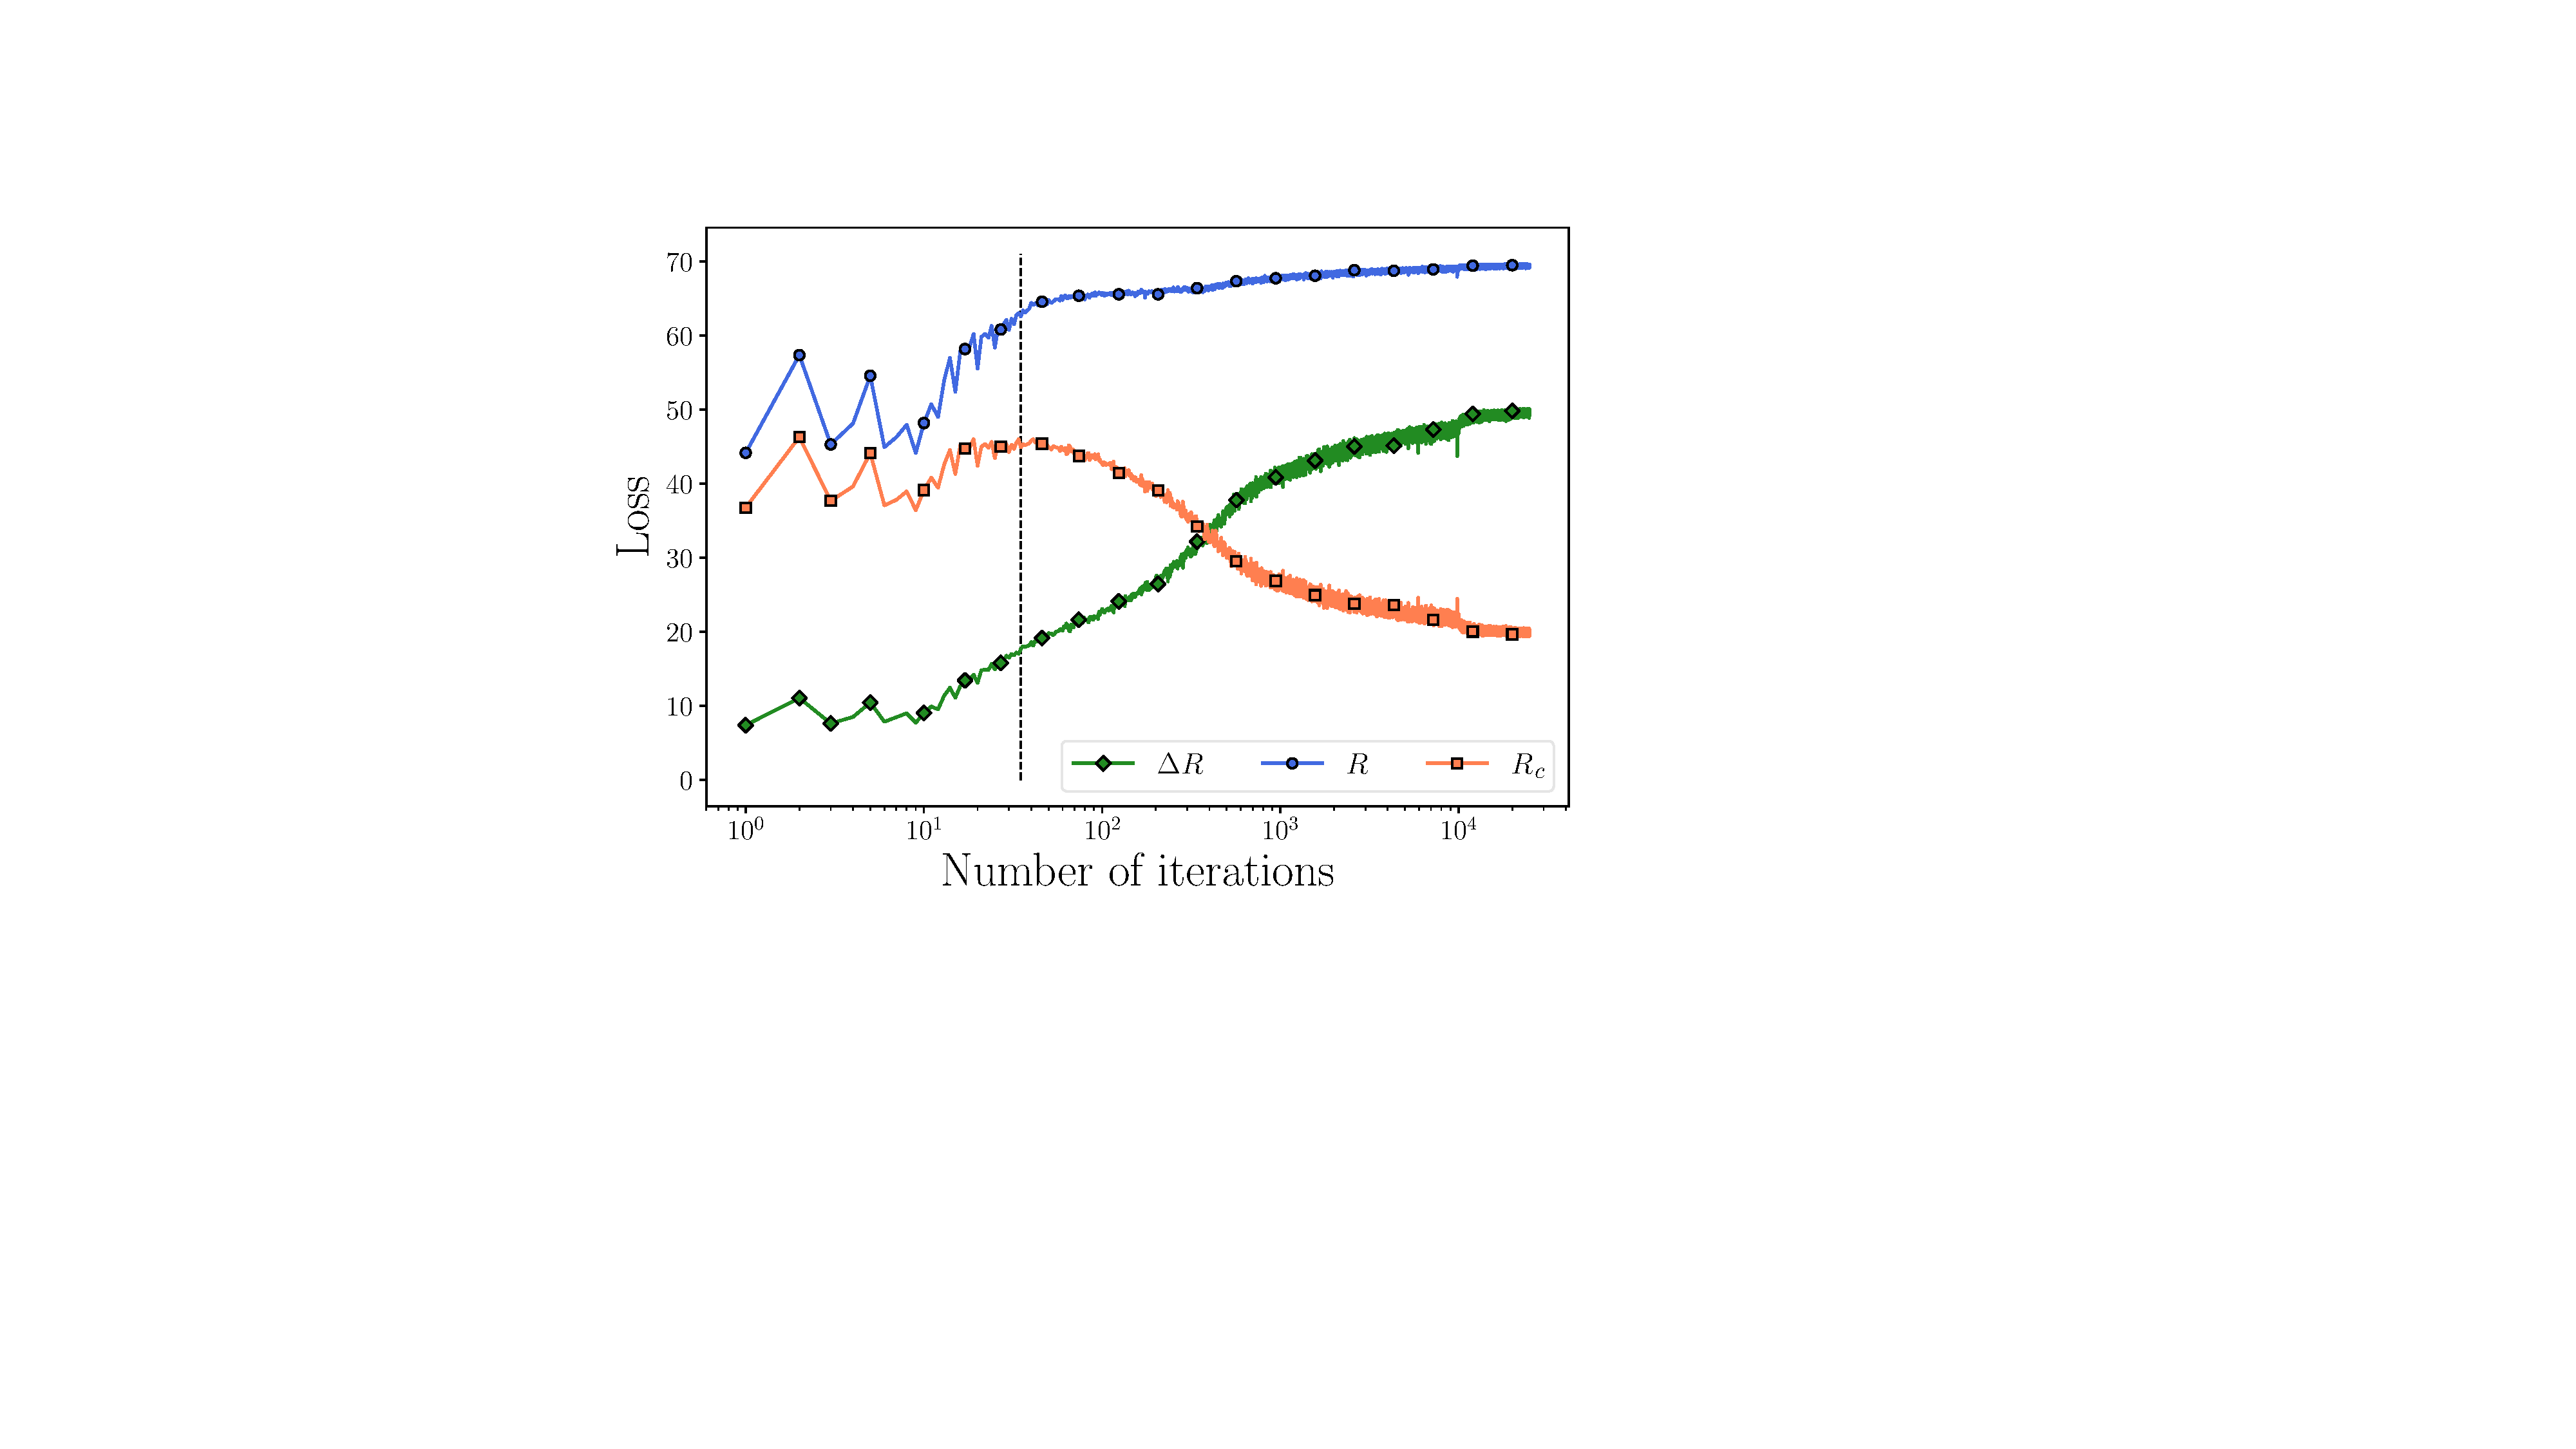
\includegraphics[width=\textwidth]{\toplevelprefix/chapters/chapter3/figs/loss_log.pdf}
			\caption{训练过程中 $R_\epsilon$, $R^c_\epsilon$, $\Delta R_\epsilon$ 的演变。}
			\label{fig:train-test-loss-pca-1}
		\end{subfigure}
		\hfill
		\begin{subfigure}[t]{0.42\textwidth}
			\centering
			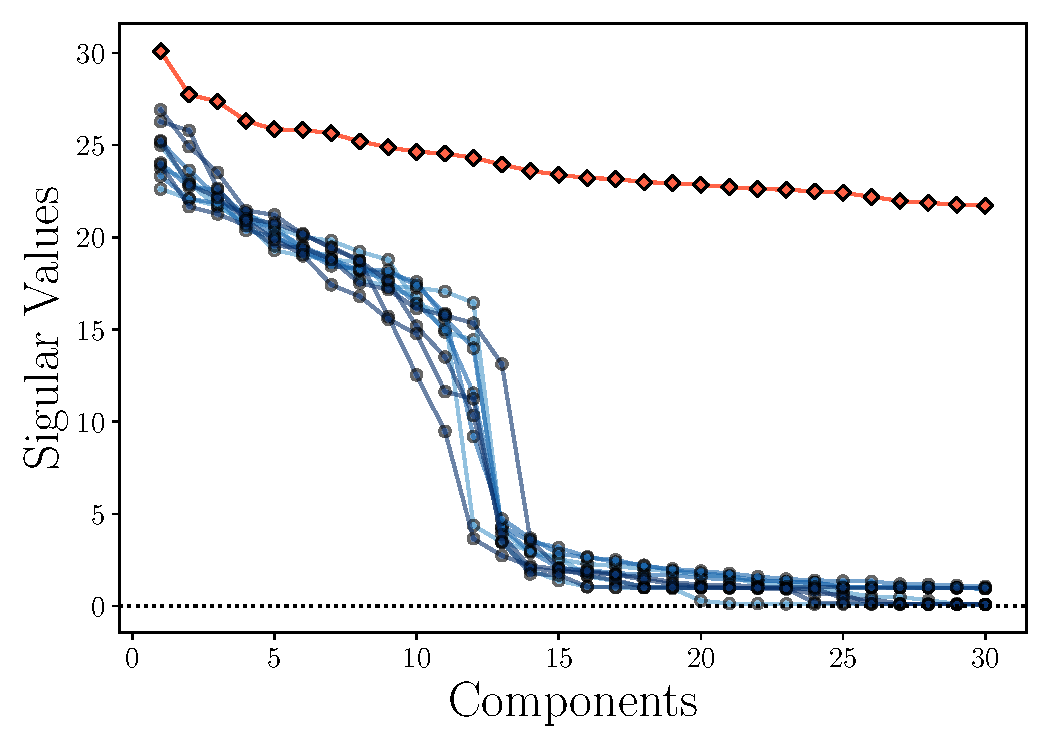
\includegraphics[width=\textwidth]{\toplevelprefix/chapters/chapter3/figs/pca_mainline.pdf}
			\caption{PCA: {\small (\textbf{红色}) 整体数据;(\textbf{蓝色}) 单个类别}。}
			\label{fig:train-test-loss-pca-3}
		\end{subfigure}
		\caption{\small 训练过程中 MCR$^2$ 率的演变,学习到的特征的主成分。}
		\label{fig:train-test-loss-pca}
	\end{figure}

	% \begin{figure}[t]
	%     %\includegraphics[width=0.47\textwidth]{chapters/chapter3/figs/heatmap_mcr2.pdf}
	%     %\includegraphics[width=0.47\textwidth]{figs_chap4/heatmap_ce.pdf}
	%     \caption{\small Cosine similarity between  learned features by using the MCR$^2$ objective  (\textbf{left}) and CE loss (\textbf{right}).}
	%     \label{fig:heatmap-plot}
	% \end{figure}

	\begin{figure*}[b]
		\begin{center}

			\includegraphics[width=0.42\textwidth]{\toplevelprefix/chapters/chapter3/figs/heatmap_mcr2.pdf}
			\hspace{0.25cm}
			\includegraphics[width=0.42\textwidth]{\toplevelprefix/chapters/chapter3/figs/heatmap_ce.png}
			\caption{\small 使用 MCR$^2$ 目标(\textbf{左})和 CE 损失(\textbf{右})学习到的特征之间的余弦相似度。}
			\label{fig:heatmap-plot}
		\end{center}
		\vskip -0.1in
	\end{figure*}

	图~\ref{fig:train-test-loss-pca-1} 说明了两个率及其差异(对于训练和测试数据)在训练的各个时期如何演变:在初始阶段之后,$R_\epsilon$ 逐渐增加,而 $R^c_\epsilon$ 减少,表明特征 $\bm Z$ 作为一个整体在扩展,而每个类别 $\bm Z_k$ 正在被压缩。
	图~\ref{fig:train-test-loss-pca-3} 显示了每个 $\Z_k$ 的奇异值分布。图~\ref{fig:heatmap-plot} 显示了按类别排序的学习到的特征之间的余弦相似度。我们比较了使用交叉熵 \eqref{chap4-eqn:cross-entropy} 和 MCR$^2$ 目标 \eqref{eqn:maximal-rate-reduction} 学习到的特征的相似性。从图中可以清楚地看到,使用 MCR$^2$ 损失学习到的表示比使用交叉熵损失学习到的表示要多样得多。这个实验的更多细节可以在 \cite{chan2021redunet} 中找到。
	%In addition, we find that we are able to select diverse images from the same class according to the ``principal'' components of the learned features (see Figure~\ref{fig:visual-class-2-8} and Figure~\ref{fig:visual-overall-data}).
	\label{eg:Rate-Reduction-CIFAR10}
\end{example}

%\yima{I would suggest the above example is better moved to the Chapter 3. To justify the rate reduction objective function and its landscape.}

然而,在上述实验中使用的网络架构明显缺乏理由。尚不清楚为什么这里采用的网络(ResNet-18)适合表示映射 $f(\x, \theta)$,更不用说解释内部学习到的层算子和参数 $\theta$ 了。在下一章中,{\em 我们将展示如何完全从期望的目标(比如说率降低)中推导出网络架构和组件,作为一个“白盒”。}



\paragraph{正则化的 MCR$^2$。}
上述定理刻画了率降低目标的全局最优解的性质。那么其他最优解,比如局部最优解呢?由于弗罗贝尼乌斯范数的约束,从优化理论的角度分析问题 \eqref{eqn1:maximal-rate-reduction} 是一项困难的任务。因此,我们考虑 \eqref{eqn1:maximal-rate-reduction} 的拉格朗日形式。这可以被看作是问题 \eqref{eqn1:maximal-rate-reduction} 的一个紧松弛甚至是等价问题,其最优解在正则化参数的特定设置下是一致的;参见 \cite[Proposition 1]{wang2024global}。
具体来说,我们研究的公式,此后称为\textit{正则化的 MCR$^2$ 问题},如下所示:
\begin{align}\label{eq:MCR-reg}
	\max_{\bm Z}\ R_{\epsilon}(\Z) - R_{\epsilon}^c(\Z) - \frac{\lambda}{2}\|\bm Z\|_F^2,
\end{align}
其中 $\lambda > 0$ 是正则化参数。尽管程序 \eqref{eq:MCR-reg} 是高度非凹的,并且在其梯度计算中涉及矩阵求逆,我们仍然可以明确地刻画其局部和全局最优解,如下所示。

\begin{theorem}[\bf 局部和全局最优解]\label{thm:mcr-global-opt}
	设 $N_k$ 表示第 $k$ 类中训练样本的数量,对于每个 $k \in \{1,\dots,K\}$,$N_{\max} \doteq \max\{N_1,\dots,N_K\}$,$\alpha=d/(N\epsilon^2)$,以及对于每个 $k \in \{1,\dots,K\}$,$\alpha_{k} = d/(N_k\epsilon^2)$。给定一个编码精度 $\epsilon > 0$,如果正则化参数满足
	\begin{align}\label{eq:lambda}
		\lambda \in \left(0, \frac{d(\sqrt{N/N_{\max}}-1)}{N(\sqrt{N/N_{\max}}+1)\epsilon^2} \right],
	\end{align}
	那么以下陈述成立: \\
	(i) ({\bf 局部最大化子}) $\bm Z^* = \left[\bm Z_1^*,\dots,\bm Z_K^* \right]$ 是问题 \eqref{eq:MCR-reg} 的一个局部最大化子,当且仅当第 $k$ 个块接受以下分解
	\begin{align}\label{eq:Zk opti}
		\bm Z_k^* = \left(\frac{ \eta_k + \sqrt{\eta_k^2 - 4\lambda^2N/N_k}}{2\lambda \alpha_{k}}\right)^{1/2} \bm U_k \bm V_k^\top,
	\end{align}
	其中 (a) $r_k = \mathrm{rank}(\bm Z_k^*)$ 满足 $r_k \in [0,\min\{N_k,d\})$ 且 $\sum_{k=1}^K r_k \le \min\{N,d\}$,(b) $\bm U_k \in \mathcal{O}^{d \times r_k}$ 满足对于所有 $k \neq l$,$\bm U_k^{\top}\bm U_l = \bm 0$,$\bm V_k \in \mathcal{O}^{N_k \times r_k}$,以及 (c) 对于每个 $k\in \{1,\dots,K\}$,$\eta_k=(\alpha_k-\alpha) - \lambda(N/N_k+1)$。
	\\
	(ii) ({\bf 全局最大化子}) $\bm Z^* = \left[\bm Z_1^*,\dots,\bm Z_K^* \right]$ 是问题 \eqref{eq:MCR-reg} 的一个全局最大化子,当且仅当 (a) 它满足上述所有条件且 $\sum_{k=1}^K r_k = \min\{m,d\}$,以及 (b) 对于所有满足 $N_k < N_l$ 和 $r_l > 0$ 的 $k \neq l \in [K]$,我们有 $r_k = \min\{N_k,d\}$。
\end{theorem}

\begin{figure}[t]
	\centering
	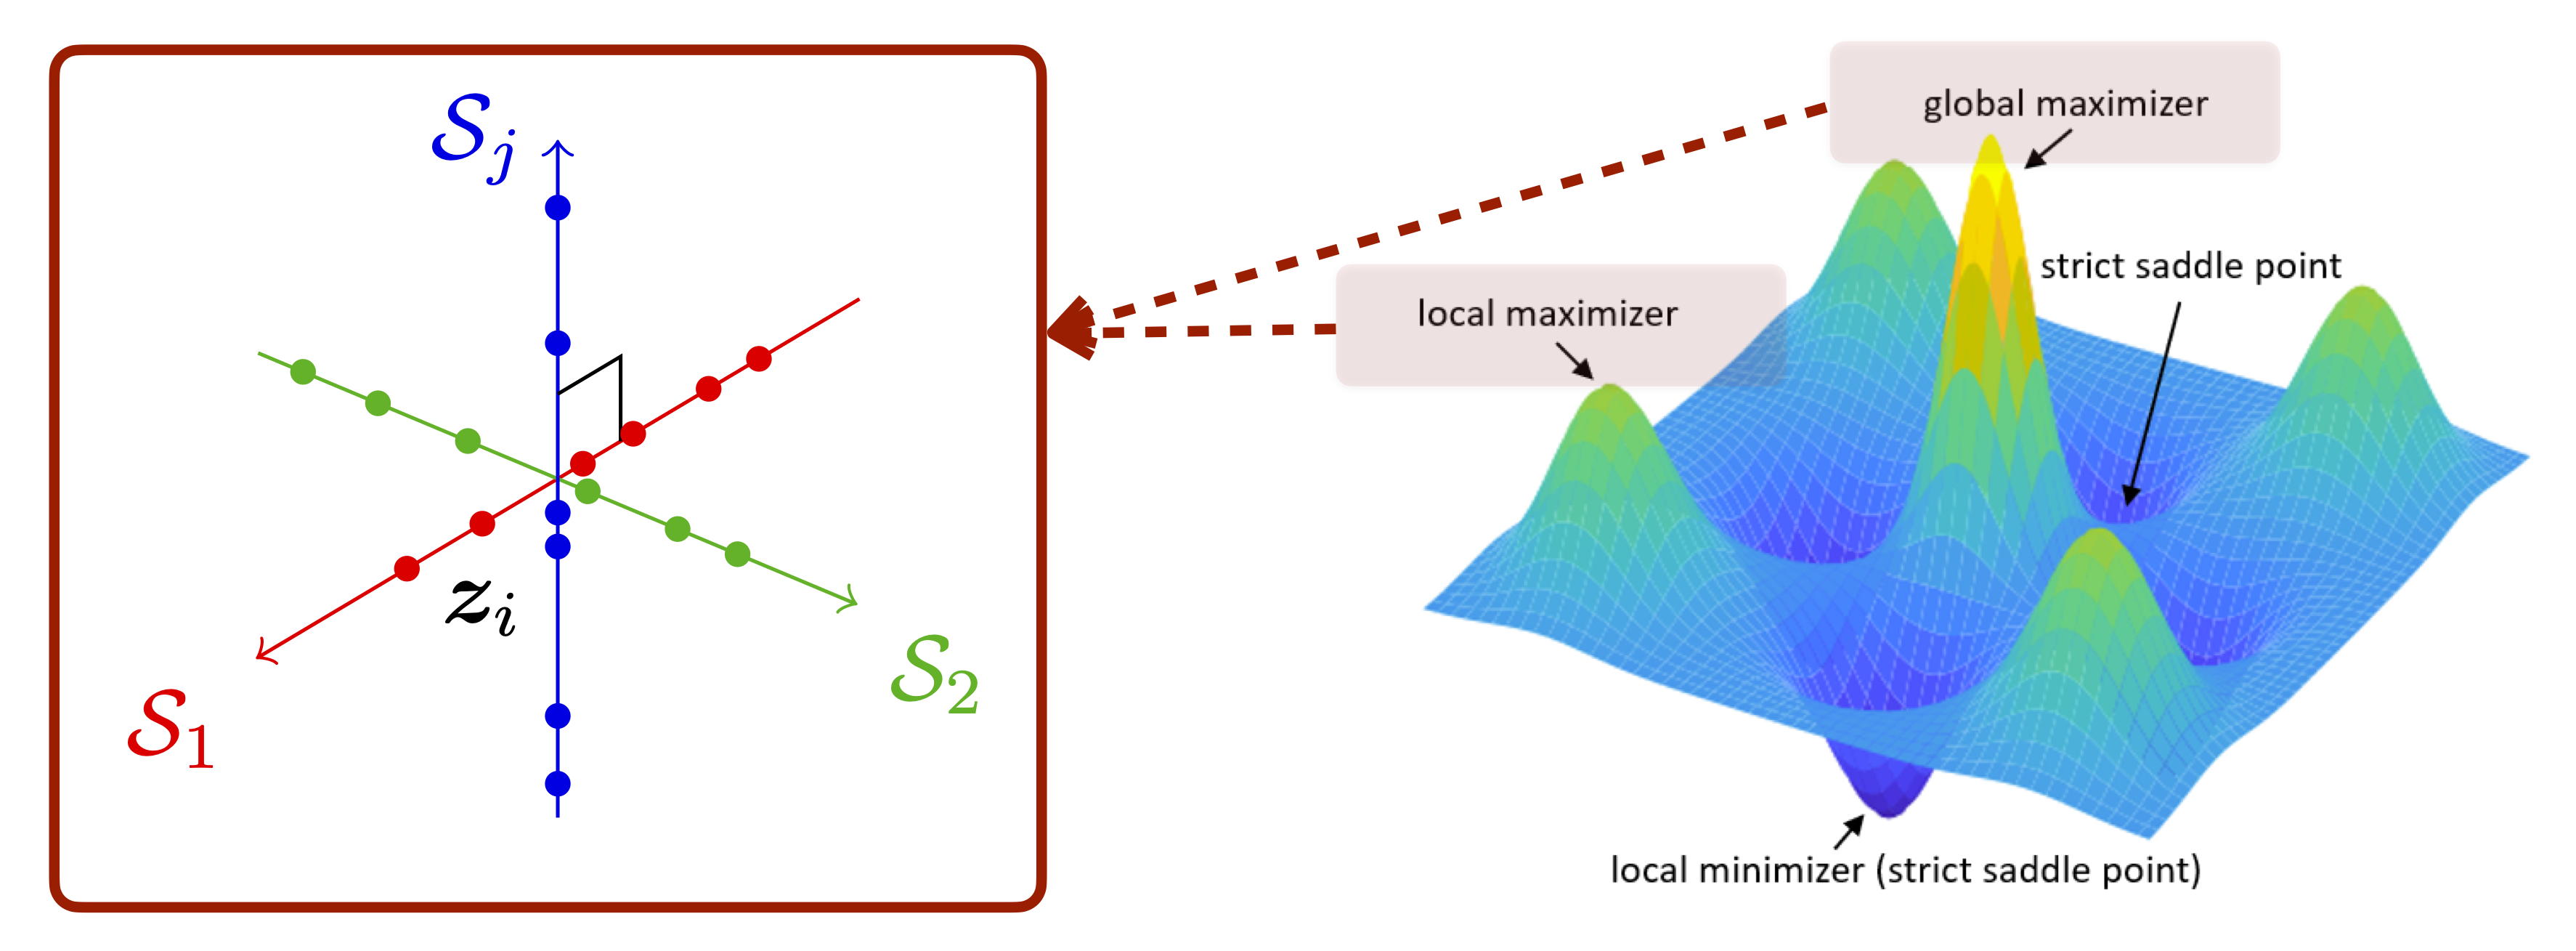
\includegraphics[width=0.8\linewidth]{\toplevelprefix/chapters/chapter3/figs/mcr2-global-local.png}
	\caption{{\bf 全局优化景观:} 根据 \cite{sun2015nonconvex,lee2016gradient},\Cref{thm:mcr-global-opt,thm:mcr-benign-opt-landscape},(正则化的)率降低目标的全局和局部最大值都对应于一个具有相互不相干子空间的解。所有其他临界点都是严格鞍点。}
	\label{fig:mcr-global-local}
\end{figure}

这个定理明确地刻画了问题 \eqref{eq:MCR-reg} 的局部和全局最优解。直观地说,这表明由问题 \eqref{eq:MCR-reg} 的每个局部最大化子表示的特征是低维和判别性的。尽管我们在定理~\ref{thm:mcr-global-opt} 中刻画了局部和全局最优解,但尚不清楚是否可以使用 GD 有效地计算这些解来解决问题 \eqref{eq:MCR-reg},因为 GD 可能会卡在其他临界点,如鞍点。
幸运的是,\cite{sun2015nonconvex,lee2016gradient} 表明,如果一个函数是二次连续可微的并且满足{\em 严格鞍点性质},即每个临界点要么是局部极小值,要么是严格鞍点\footnote{我们说一个临界点是问题 \eqref{eq:MCR-reg} 的一个严格鞍点,如果它有一个具有严格正曲率的方向~\cite{sun2015nonconvex}。这包括具有严格正曲率的经典鞍点以及局部极小值。},那么 GD 从随机初始化开始几乎肯定会收敛到其局部极小值。我们通过刻画问题 \eqref{eq:MCR-reg} 的所有临界点来研究其全局优化景观,如下所示。

 \begin{theorem}[\bf 良性全局优化景观]\label{thm:mcr-benign-opt-landscape}
	给定一个编码精度 $\epsilon > 0$,如果正则化参数满足 \eqref{eq:lambda},那么问题 \eqref{eq:MCR-reg} 的任何临界点 $\bm Z$ 要么是一个局部最大化子,要么是一个严格鞍点。
\end{theorem}
总之,上述两个定理表明,与率降低目标的每个局部最大化子(不仅仅是全局最大化子)相关的学习到的特征被构造成不相干的低维子空间。此外,(正则化的)率降低目标 \eqref{eqn:maximal-rate-reduction} 具有一个非常良性的景观,只有局部最大值和严格鞍点作为临界点,如图 \ref{fig:mcr-global-local} 所示。
% To our knowledge, \Cref{thm:mcr-global-opt,thm:mcr-benign-opt-landscape} constitute the first analysis of local optima and optimization landscapes for MCR$^2$ objectives. 
根据 \cite{sun2015nonconvex,lee2016gradient},\Cref{thm:mcr-global-opt,thm:mcr-benign-opt-landscape} 意味着可以通过从随机初始化开始对率降低目标 \eqref{eqn:maximal-rate-reduction} 应用(随机)梯度下降来有效地找到低维和判别表示(LDR)。这些结果也间接解释了为什么在示例 \ref{eg:Rate-Reduction-CIFAR10} 中,如果选择的网络足够富有表现力并且训练得很好,得到的表示通常会给出一个不相干的线性表示,这很可能对应于全局最优解。
感兴趣的读者可以参考 \cite{wang2024global} 获取证明。



%\subsection{Classification via minimal incremental coding length}
%\href{http://people.eecs.berkeley.edu/~yima/psfile/MICL_SJIS.pdf}{supervised classification} from the perspective of (lossy) compression.

\section{总结与注释}

使用去噪和扩散进行采样的历史非常丰富。第一个明确关于扩散模型的工作可能是 \cite{Sohl-Dickstein2015},但在此之前,有许多关于去噪作为计算和统计问题的工作。其中最相关的可能是 \cite{hyvarinen05a},它明确使用分数函数进行去噪(以及执行独立成分分析)。最流行的后续工作基本上是同时出现的:\cite{ho2020denoising,song2019}。从那时起,成千上万的论文建立在扩散模型之上;我们将在 \Cref{ch:autoencoding} 中重新讨论这个主题。

许多这些工作使用的随机过程与简单的线性组合 \eqref{eq:gen_additive_gaussian_noise_model} 不同。事实上,上面列出的所有工作都强调了在前向过程的每一步开始时添加\textit{独立的}高斯噪声的必要性。理论导向的工作实际上使用布朗运动或随机微分方程来构建前向过程 \cite{song2020score}。然而,由于高斯的线性组合仍然是高斯,这些过程的\textit{边际分布}仍然采用 \eqref{eq:gen_additive_gaussian_noise_model} 的形式。我们的大部分讨论只需要边际分布是它们的样子,因此我们过于简化的模型实际上对于几乎所有事情都足够了。事实上,唯一边际分布不够的时候是我们推导 \(\Ex[\vx_{s} \mid \vx_{t}]\) 关于 \(\Ex[\vx \mid \vx_{t}]\) 的表达式时。不同的(加噪)过程给出不同的此类表达式,这些表达式可以用于采样(当然还有其他方法可以推导出高效的采样器,例如一直很流行的 DDPM 采样器)。\eqref{eq:gen_additive_gaussian_noise_model} 中的过程是一个真正的随机过程,然而,其“自然”的去噪迭代采用流行的 DDIM 算法的形式 \cite{song2020denoising}。(即使是这种等价性也不是微不足道的;我们引用 \cite{de2025distributional} 作为理由。)

% {Lossy coding does more than just quantization. It allows us to avoid a pathological solution by simply using the empirical distribution as the optimal solution that minimizes entropy. }

% {From the achievable (entropy) to an implementable coding scheme. That is, in addition to a computable or achievable encoding scheme, there should also exist an implementable decoding scheme. Lossy quantization becomes necessary for real-valued data.} 

除了在 \Cref{sec:denoising-intro} 中介绍的理论工作 \citep{li2024d},以及它所建立的一系列工作,这些工作研究了当数据具有低维结构时扩散模型的\textit{采样}效率,还有大量的工作研究了当数据具有低维结构时扩散模型的\textit{训练}效率。具体来说,\citet{chen2023score} 和 \citep{wang2024diffusion} 刻画了当数据属于低秩高斯混合模型时去噪器的近似和估计误差,表明准确学习分布所需的训练样本数量与数据的内在维度而不是环境维度成比例。有相当多的\textit{方法论}工作试图利用数据的低维结构来用扩散模型做各种事情。我们在这里重点介绍三个:图像编辑 \citep{chen2024exploring}、水印 \citep{li2024shallow} 和遗忘学习 \citep{chen2025dual},尽管这总是一个不详尽的列表。
 
% On top of the work \citep{li2024adapting} covered in \Cref{sec:denoising-intro}, many studies have drawn increasing attention to the training and sampling efficiency of diffusion models when the image data has low-dimensional structures. On the training side, \cite{chen2023score} provided a theoretical framework for understanding how diffusion models perform when the data lie on or near low-dimensional manifolds. It rigorously analyzes the approximation and estimation errors of score functions under manifold settings and demonstrates that diffusion models can achieve efficient distribution recovery with sample and computational complexities that depend on the intrinsic, rather than ambient, dimensionality of the data. Later, \cite{wang2024diffusion} extended the analysis and provided compelling theoretical and empirical evidence that diffusion models can be trained efficiently when the data distribution lies near a union of low-dimensional subspaces. Specifically, they show that the number of training samples required to accurately learn a mixture of low-rank Gaussian distributions scales linearly with the intrinsic dimension of the data. These works indicate that diffusion models are capable of leveraging low-dimensional structures inherent in image data, leading to significant improvements in training efficiency. On the sampling side, \cite{li2024adapting} showed that when the underlying distribution lies on or near a low-dimensional manifold in the high-dimensional space, denosing diffusion probabilistic model (DDPM) sampler can adapt to low-dimensional structures and achieves a sampling rate at the order of $O(k^2/\sqrt{T})$, where $k$ is the instinct dimension and $T$ is the number of steps. Recently, \cite{liang2025low} analyzed how diffusion generative models leverage unknown low-dimensional structures to accelerate sampling. They showed that the DDPM sample achieves a sampling rate at the order of $O(k/T)$. \cite{tang2024adaptivity} showed that both Langevin diffusion and forward-backward diffusion models can adapt to the intrinsic manifold structure and the sampling rate of the inducing distribution estimator depends only on the intrinsic dimension of the data. These results collectively demonstrate that diffusion models can effectively exploit intrinsic low-dimensional structures in the data to significantly improve sampling efficiency. 











% \pw{Add some references on computational and sampling efficiency of diffusion models and discuss these results.}




\section{练习与扩展}

\begin{exercise}
    请证明 \eqref{eq:optimal_denoiser} 是问题 \eqref{eq:denoising_loss} 的最优解。
\end{exercise}

\begin{exercise}\label{exercise:conditional_gaussian}
  考虑随机向量 $\vx \in \bR^D$ 和 $\vy \in \bR^d$,使得对 $(\vx, \vy) \in \bR^{D + d}$ 是联合高斯的。这意味着
  \begin{equation*}
    \begin{bmatrix}
      \vx \\
      \vy
    \end{bmatrix}
    \sim
    \cN \left(
      \begin{bmatrix}
        \vmu_{\vx} \\
        \vmu_{\vy}
      \end{bmatrix}
      ,
      \begin{bmatrix}
        \vSigma_{\vx} & \vSigma_{\vx\vy} \\
        \vSigma_{\vx\vy}^\top & \vSigma_{\vy}
      \end{bmatrix}
    \right),
  \end{equation*}
  其中均值和协方差参数由下式给出
  \begin{equation*}
    \vmu_{\vx} = \bE[\vx],\quad \vmu_{\vy} = \bE[\vy],\quad
    \begin{bmatrix}
      \vSigma_{\vx} & \vSigma_{\vx\vy} \\
      \vSigma_{\vx\vy}^\top & \vSigma_{\vy}
    \end{bmatrix}
    =
    \bE\left[
      \begin{bmatrix}
        \vx - \bE[\vx] \\
        \vy - \bE[\vy]
      \end{bmatrix}
      \begin{bmatrix}
        \vx - \bE[\vx] \\
        \vy - \bE[\vy]
      \end{bmatrix}^\top
      \right]
  \end{equation*}
  假设 $\vSigma_{\vy}$ 是正定的(因此是可逆的);那么协方差矩阵的正半定性等价于舒尔补条件 $\vSigma_{\vx} - \vSigma_{\vx\vy} \vSigma_{\vy}^{-1}
  \vSigma_{\vx\vy}^\top \succeq \Zero$。

  在本练习中,我们将证明条件分布 $p_{\vx \mid
  \vy}$ 是高斯的:即
  \begin{equation}\label{eq:gaussian-conditional-eqn}
    p_{\vx \mid \vy} \sim \cN\left(
      \vmu_{\vx} + \vSigma_{\vx\vy} \vSigma_{\vy}^{-1} (\vy - \vmu_{\vy}),
      \vSigma_{\vx} - \vSigma_{\vx\vy} \vSigma_{\vy}^{-1}
      \vSigma_{\vx\vy}^{\top}
    \right).
  \end{equation}
  证明这个结果的一个直接途径是操纵密度的定义比率 $p_{\vx, \vy} / p_{\vy}$。我们下面勾勒出这种形式的一个代数上简洁的论证。

  \begin{enumerate}
    \item 验证协方差的以下矩阵恒等式:
      \begin{equation}\label{eq:gaussian-conditional-covariance-block}
        \begin{bmatrix}
          \vSigma_{\vx} & \vSigma_{\vx\vy} \\
          \vSigma_{\vx\vy}^\top & \vSigma_{\vy}
        \end{bmatrix}
        =
        \begin{bmatrix}
          \vI_D & \vSigma_{\vx\vy}\vSigma_{\vy}^{-1} \\
          \Zero & \vI_d
        \end{bmatrix}
        \begin{bmatrix}
          \vSigma_{\vx} - \vSigma_{\vx\vy} \vSigma_{\vy}^{-1}
          \vSigma_{\vx\vy}^{\top} & \Zero \\
          \Zero & \vSigma_{\vy}
        \end{bmatrix}
        \begin{bmatrix}
          \vI_D & \Zero\\
          \vSigma_{\vy}^{-1}\vSigma_{\vx\vy}^\top & \vI_d
        \end{bmatrix}.
      \end{equation}
      这个恒等式是通过对协方差矩阵进行两轮(分块)高斯消元得到的。
    \item 基于前面的恒等式,证明
      \begin{equation}\label{eq:gaussian-conditional-covariance-inverse-block}
        \begin{bmatrix}
          \vSigma_{\vx} & \vSigma_{\vx\vy} \\
          \vSigma_{\vx\vy}^\top & \vSigma_{\vy}
        \end{bmatrix}^{-1}
        =
        \begin{bmatrix}
          \vI_D & \Zero\\
          -\vSigma_{\vy}^{-1}\vSigma_{\vx\vy}^\top & \vI_d
        \end{bmatrix}
        \begin{bmatrix}
          \left(\vSigma_{\vx} - \vSigma_{\vx\vy} \vSigma_{\vy}^{-1}
          \vSigma_{\vx\vy}^{\top}\right)^{-1} & \Zero \\
          \Zero & \vSigma_{\vy}^{-1}
        \end{bmatrix}
        \begin{bmatrix}
          \vI_D & -\vSigma_{\vx\vy}\vSigma_{\vy}^{-1} \\
          \Zero & \vI_d
        \end{bmatrix}
      \end{equation}
      只要相关的逆矩阵有定义。\footnote{在舒尔补项不可逆的情况下,同样的结果也成立,其逆矩阵被摩尔-彭罗斯伪逆代替。特别是,条件分布 \eqref{eq:gaussian-conditional-eqn} 变成一个退化的高斯分布。}
      得出结论
      \begin{align}
        &\begin{bmatrix}
          \vx-\vmu_{\vx} \\
          \vy-\vmu_{\vy}
        \end{bmatrix}^{\top}
        \begin{bmatrix}
          \vSigma_{\vx} & \vSigma_{\vx\vy} \\
          \vSigma_{\vx\vy}^\top & \vSigma_{\vy}
        \end{bmatrix}^{-1}
        \begin{bmatrix}
          \vx-\vmu_{\vx} \\
          \vy-\vmu_{\vy}
        \end{bmatrix}
        \\
        &\qquad=
        \begin{bmatrix}
          \vx - \left(\vmu_{\vx} + \vSigma_{\vx\vy}\vSigma_{\vy}^{-1}(\vy
          - \vmu_{\vy})\right) \\
          \vy - \vmu_{\vy}
        \end{bmatrix}^\top
        \begin{bmatrix}
          \left(\vSigma_{\vx} - \vSigma_{\vx\vy} \vSigma_{\vy}^{-1}
          \vSigma_{\vx\vy}^{\top}\right)^{-1} & \Zero \\
          \Zero & \vSigma_{\vy}^{-1}
        \end{bmatrix}
        \begin{bmatrix}
          \vx - \left(\vmu_{\vx} + \vSigma_{\vx\vy}\vSigma_{\vy}^{-1}(\vy
          - \vmu_{\vy})\right) \\
          \vy - \vmu_{\vy}
        \end{bmatrix}.
      \end{align}
      (\textit{提示:为了简化代数运算,请注意 \Cref{eq:gaussian-conditional-covariance-block} 右侧的第一个和最后一个矩阵是彼此的转置。})
    \item 通过除以 $p_{\vx, \vy} / p_{\vy}$,证明 \Cref{eq:gaussian-conditional-eqn}。(\textit{提示:使用前面的恒等式,只需要最少的代数运算。对于归一化常数,使用 \Cref{eq:gaussian-conditional-covariance-inverse-block} 来类似地分解行列式。})

  \end{enumerate}


\end{exercise}

\begin{exercise}\label{exercise:sherman_morrison_woodbury_identity}
    证明 Sherman-Morrison-Woodbury 恒等式,即对于矩阵 \(\vA\)、\(\vC\)、\(\vU\)、\(\vV\),使得 \(\vA\)、\(\vC\) 和 \(\vA + \vU\vC\vV\) 是可逆的,
    \begin{equation}
        (\vA + \vU\vC\vV)^{-1} = \vA^{-1} - \vA^{-1}\vU(\vC^{-1} + \vV\vA^{-1}\vU)^{-1}\vV\vA^{-1}
    \end{equation}
\end{exercise}

\begin{exercise}\label{exercise:generalizing_results_to_different_noise_models}
    假设 \(\vx_{t}\) 遵循广义噪声模型 \eqref{eq:gen_additive_gaussian_noise_model},重新推导以下内容。
    \begin{itemize}
        \item 特威迪公式:\eqref{eq:gen_tweedie}。
        \item DDIM 迭代:\eqref{eq:gen_denoising_iteration}。
        \item 高斯混合模型的贝叶斯最优去噪器:\eqref{eq:gen_gmm_bayes_optimal_denoiser}。
    \end{itemize}
\end{exercise}

\begin{exercise}\label{exercise:implement_denoising_processes}
\begin{enumerate}
    \item 实现 \Cref{exercise:generalizing_results_to_different_noise_models} 中推导的公式,构建一个高斯混合的采样器。
    \item 复现 \Cref{fig:ve_forward_denoising} 和 \Cref{fig:vp_gmm_denoising}。
    \item 我们现在引入一个独立的过程,称为\textit{流匹配(FM)},如下所示:
    \begin{equation}
        \alpha_{t} = 1 - t, \qquad \sigma_{t} = t.
    \end{equation}
    使用相同的框架实现这个过程,并测试其在高维采样中的效果。哪个过程似乎能给出更好或更稳定的结果?
\end{enumerate}
\end{exercise}

% \begin{exercise}\label{exer:prop cover}
% 	Prove \Cref{thm:covering-number-rate-distortion}. Recall that we had \(\vx\) a random variable with compact support \(K\).
% 	\begin{enumerate}
% 		\item First, prove that the covering number \(\cN\) and rate distortion
% 		\(\cR\) (refer to \Cref{thm:covering-number-rate-distortion} for the definition of the covering number) have the following inequality:
% 		\begin{equation}
% 			\cR_{\epsilon}(\vx) \leq \log_{2} \cN_{\epsilon}(K).
% 		\end{equation}
% 		\item Second, show that this inequality is \textit{tight} when \(\vx\) is uniformly distributed on \(K\).
% 		\item Third, show that there is \textit{no} lower bound in general of the form \(\log_{2} \cN_{c\epsilon}(K) \leq \cR_{\epsilon}(\vx)\) for any constant \(c > 0\). \textit{Hint:} Suppose that \(\vx\) takes finitely many values for simplicity, suppose that these values are very spread out, and it takes one of these values with very high probability. Depending on how you precisely define \(\vx\), the optimal coding scheme is just this high-probability value itself, and so the rate distortion functionin this case is \(0\). Meanwhile, the covering number can be large. Fill in the details to complete this part of the problem.
% 	\end{enumerate}
% \end{exercise}

\begin{exercise}
	请证明以下关于 $\log\det(\cdot)$ 函数的性质。
	\begin{enumerate}
		\item 证明
		      \begin{align*}
			      f(\vX) = \log\det\left(\vX\right)
		      \end{align*}
		      是一个凹函数。({\bf 提示:} 函数 $f(\vx)$ 是凸的当且仅当对于所有 $\vx$ 和 $\vh$,函数 $f(\vx+t\vh)$ 是凸的。)

		\item 证明:
		      \begin{align*}
			      \log\det(\vI + \vX^\top\vX) = \log\det(\vI + \vX\vX^\top)
		      \end{align*}

		\item 设 $\vA \in \R^{n\times n}$ 是一个正定矩阵。请证明:
		      \begin{align}
			      \log\det\left(\vA \right) = \sum_{i=1}^n \log(\lambda_i),
		      \end{align}
		      其中 $\lambda_1,\lambda_2,\dots,\lambda_n$ 是 $\vA$ 的特征值。
	\end{enumerate}

\end{exercise}

% \begin{exercise}
% 	\sdb{Exercise about proving the Gaussian is max entropy (in a remark in
% 		appendix B rn)}
% \end{exercise}

 

\end{document}{exercise}
% 	\sdb{Exercise about proving the Gaussian is max entropy (in a remark in
% 		appendix B rn)}
% \end{exercise}

 

\end{document}